\documentclass[12pt]{article}
 
\usepackage[margin=1in]{geometry} 
\usepackage{amsmath,amsthm,amssymb,graphicx,mathtools,tikz,float,mathrsfs,multicol,textcomp,gensymb,extarrows,dsfont,tikz-cd,subcaption,enumerate,blkarray,cancel,epigraph,xcolor,ytableau}
\usepackage[urlcolor=blue]{hyperref}
\hypersetup{
    colorlinks   = true,
    citecolor    = gray,
    linkcolor    = blue
} % Lime green, really?! Not only is that a sore sight, lime green has been an enemy of mine since 2007.
\usetikzlibrary{positioning}
\newcommand{\n}{\mathbb{N}}
\newcommand{\z}{\mathbb{Z}}
\newcommand{\q}{\mathbb{Q}}
\newcommand{\cx}{\mathbb{C}}
\newcommand{\real}{\mathbb{R}}
\newcommand{\h}{\mathbb{H}}
\newcommand{\field}{\mathbb{F}}
\newcommand{\ita}[1]{\textit{#1}}
\newcommand{\oneton}[1]{\{1,\dotsc,#1\}}
\newcommand\Idea[1]{\begin{gather*}#1\end{gather*}}
\newcommand\proofs[1]{\begin{proof}#1\end{proof}}
\newcommand\inv[1]{#1^{-1}}
\newcommand\paren[1]{\left( #1 \right)}
\newcommand\setb[1]{\left \{ #1 \right \}}
\newcommand{\vbrack}[1]{\left \langle #1 \right \rangle}
\newcommand{\spank}[1]{\mathrm{span}_{#1}}
\newcommand{\quotient}[2]{{\makebox[\width-2.3pt][l]{\raisebox{.2em}{$#1$}}\left/\raisebox{-.2em}{$#2$}\right.}}

\newtheorem{theorem}{Theorem}[section]
\newtheorem{proposition}[theorem]{Proposition}
\newtheorem{corollary}[theorem]{Corollary}
\newtheorem{lemma}[theorem]{Lemma}
\newtheorem*{claim}{Claim}
\theoremstyle{definition}
\newtheorem{definition}[theorem]{Definition}
\newtheorem*{remark}{Remark}
\newtheorem{example}{Example}[section]

\allowdisplaybreaks
\usepackage[shortlabels]{enumitem}

\tikzset{
  symbol/.style={
    draw=none,
    every to/.append style={
      edge node={node [sloped, allow upside down, auto=false]{$#1$}}}
  }
}

\DeclareMathOperator\Aut{Aut}
\DeclareMathOperator\End{End}
\DeclareMathOperator\Hom{Hom}
\DeclareMathOperator\Id{Id}
\DeclareMathOperator\im{Im}
\newcommand{\m}{\mathbb{M}}
\DeclareMathOperator\tr{tr}
\DeclareMathOperator\GL{GL}
\DeclareMathOperator\sgn{sgn}

\begin{document}
\date{Spring 2020} 
\author{typeset by Alexander Louis J. Sabater}
\title{MATH 545: Representation Theory Course Notes}
\maketitle
\newpage
\tableofcontents
\newpage
\begin{abstract}
    These are the course notes from Dr. Will Murray's MATH 545 course taught in Spring 2020. I have tried to include the miniquizzes (now called blitzes) for each course meeting, but there are a few still missing. I have also tried to be as consistent with his notation (with some slight modifications of my own), including the names of theorems. The equation numbers are a mess; I'm not sure if I want to go back and fix them. Rami, you remake the plots.
\end{abstract}
\section{January 22}
\subsection{Blitz}
How many Sylow 2-subgroups does $S_4$ have?
\subsection{Overview of the Course}
\textbf{Representation Theory} is the study of groups acting on vector spaces by linear transformations.
\begin{example}
    Consider the dihedral group 
    \begin{equation}
        D_4\coloneqq \vbrack{r,s\mid r^4=s^2=e,srs=r^{-1}}.
    \end{equation}
    And yes, we write $D_n$ instead of $D_{2n}$, unlike the Philistine notation of Dummit and Foote \cite{Dummit}!
    
    As undergrads, we thought of $D_4$ as the symmetries of a rigid square (here we're thinking of the unit square in the plane $[0,1]\times[0,1]$). But what if $D_4$ drags all of $\real^2$ around with it? Then $g\in D_4$ is a linear transformation of $\real^2$; for example:
    \begin{equation}
        r\xlongleftrightarrow{}
        \begin{bmatrix}
            0 & -1 \\
            1 & 0
        \end{bmatrix}.
    \end{equation}
    Here we're rotating \ita{counterclockwise}.
\end{example}
Here is the outline for the semester:
\begin{enumerate}
    \item Definitions and examples
    \item Operations: subtraction, division, addition, multiplication
    \item Decomposition (Maschke)
    \item Semisimple modules and rings
    \item Characters
    \item Restriction and induction (full groups $\xlongleftrightarrow{}$ subgroups)
    \item $S_n$ over $\cx$
\end{enumerate}
\subsection{Endomorphisms}
For any mathematical object $T$, an \textbf{endomorphism} of $T$ is a function $f:T\to T$ that preserves whatever structure you're studying on $T$:
\begin{enumerate}
    \item If you're studying $T$ as a group, then $f$ preserves the group operation:
    \begin{equation}
        f(t_1\ast t_2)=f(t_1)\ast f(t_2).
    \end{equation}
    \item If you're studying $T$ as a ring, then $f$ preserves the two operations:
    \begin{equation}
        f(t_1+t_2)=f(t_1)+f(t_2),\qquad f(t_1t_2)=f(t_1)f(t_2).
    \end{equation}
    \item If you're studying $T$ as a set, then we have no operations. So $f$ is just a function. 
\end{enumerate}
An \textbf{automorphism} is an endomorphism that is also a bijection (so it is invertible), and so its inverse must also preserve the structure. By Homework 1, Problem 1, we actually only need to check bijectivity.
\begin{enumerate}[resume]
    \item If you're studying $T$ as a vector space over a field $k$ (or more generally as a module over a ring $R$), then $f$ preserves addition and scalar multiplication:
    \begin{equation}
        f(t_1+t_2)=f(t_1)+f(t_2),\qquad f(rt)=rf(t).
    \end{equation}
\end{enumerate}
There's something jarring about the scalar $r\in R$ clashing with the endomorphism $f$. We'll adopt an \textbf{elegant convention}: write functions on the left and scalars on the right, so we'll speak of a \ita{right} $R$-module $T_R$:
\begin{equation}
    f(tr)=f(t)r.
\end{equation}
We can add and multiply endomorphisms of a module:
\begin{equation}
    \begin{split}
        (f+g)(t)&\coloneqq f(t)+g(t)\\
        (fg)(t)&\coloneqq (f\circ g)(t)=f(g(t)).
    \end{split}
\end{equation}
All the usual rules apply (for example, $f(g+h)=fg+fh$), so we have an \textbf{endomorphism ring} $\End(T_R)$. This ring is often noncommutative, even if $R$ is a nice fluffy commutative. In fact, we have the \underline{law of the jungle}: modules over nicer rings $R$ tend to have wilder endomorphism rings $\End(T_R)$, and vice versa. This is because fewer scalars means fewer \ita{restrictions} on endomorphisms.

What do we mean by nicer? While not an actual ordering, we tend to say commutative rings are nicer than noncommutative rings, and that not having zero-divisors is nicer than having them. For example, let's look at a special case: the ring is a field $k$ (this is \ita{really} nice), so the module is a vector space $V_k$. We know (thank you Zorn!) that $V_k$ has a \underline{basis}. If $V_k$ has a \underline{finite} basis $\{v_1,\dotsc,v_n\}$, then every element $v\in V$ has a \underline{unique} representation
\begin{equation}
    v=v_1\alpha_1+\dotsb+v_n\alpha_n,
\end{equation}
so we can identify 
\begin{equation}
    v\xlongleftrightarrow{}
    \begin{bmatrix}
        \alpha_1 \\
        \vdots \\
        \alpha_n
    \end{bmatrix}.
\end{equation}
So we keep track of $V$ with the set of $n\times1$ column vectors over $k$.

What functions $f:V\to V$ respect (``commute with'') addition and (right) scalar multiplication from $k$? Such functions are given by left multiplication by matrices:
\begin{equation}
    \begin{bmatrix}
        \cdot & \cdot & \cdot \\
        \cdot & \cdot & \cdot \\
        \cdot & \cdot & \cdot 
    \end{bmatrix}
    \begin{bmatrix}
        \cdot \\
        \cdot \\
        \cdot
    \end{bmatrix}
    =
    \begin{bmatrix}
        \cdot \\
        \cdot \\
        \cdot 
    \end{bmatrix}.
\end{equation}
\begin{theorem}
    If $\dim_kV=n$, then $\End(V_k)\simeq\m_n(k)$.
\end{theorem}
What are the \underline{trivial endomorphisms}? Given $\alpha\in k$, scalar multiplication by $\alpha$ is itself an endomorphism, corresponding to the matrix
\begin{equation}
    \begin{bmatrix}
        \alpha & 0 & \cdots & 0 \\
        0 & \alpha & \cdots & 0 \\
        \vdots  & \vdots  & \ddots & \vdots  \\
        0 & 0 & \cdots & \alpha 
    \end{bmatrix}.
\end{equation}
So we always have $k\subset\m_n(k)$.
%monky
Let's not get too excited here. We have a \underline{horsefly in the ointment}: we started with a basis for $V_k$. But a vector space has \ita{many} bases with no canonical way to distinguish one of them. With different bases, each function will correspond to a different matrix.

How different? They will be related by a \textbf{change of basis matrix} $C$: given $\phi,\psi:\End(V_k)\xlongrightarrow{\sim}\m_n(k)$, there exists an invertible $C\in\m_n(k)$ such that for all $f\in\End(V_k)$, we have $\psi(f)=C^{-1}\phi(f)C$.

How about automorphisms? Invertible endomorphisms correspond to invertible matrices: $\Aut(V_k)\simeq\m_n(k)^{\times}=\GL_n(k)$. But still, it \ita{depends} on your choice of basis.

Now, what about that bit with the law of the jungle? In our case $k$ is a field, as nice as it gets, but $\End(V_k) \simeq \m_n(k)$ is not commutative and has zero divisors, which is pretty far from being as nice as a field.
\subsection{Group Actions on Sets}
Let $G$ be a group, $S$ a set. We have two equivalent definitions of a group action:
\begin{enumerate}
    \item As a binary operation $\cdot:G\times S\to S$ that respects the group arithmetic:
    \begin{enumerate}
        \item $e_Gs=s$ for all $s\in S$,
        \item $(g_1g_2)s=g_1(g_2s)$ for all $g_1,g_2\in G$, $s\in S$.
    \end{enumerate}
    \item As a group homomorphism $G\to\Aut S$. Recall that $\Aut S$ is the set of bijections on $S$. If $|S|=n<\infty$, then $\Aut S\simeq S_n$, so a group action is just a homomorphism $G\to S_n$.
\end{enumerate}
\underline{Think}: each $g\in G$ ``stirs around,'' \ita{i.e.}, permutes the elements of $S$ in a way that is consistent with the group structure. It's also consistent with the set structure, vacuously. In this course, we will replace $S$ with a vector space.
\section{January 27}
\subsection{Blitz}
It $T_R$ is a right module over a ring $R$ and $f:T_R\to T_R$ is a module homomorphism, then $f$ should satisfy?
\subsection{Definition of Representation and Examples}
\begin{definition}
    Let $V$ be a vector space over a field $k$, usually finite-dimensional. Let $G$ be a group, usually finite. We have several essentially equivalent definitions of a \textbf{representation of $G$ on $V$}:
    \begin{enumerate}
        \item A binary operation $G\times V\to V$ that respects the group arithmetic and the vector space structure.
        \begin{enumerate}
            \item Each $g\in G$ acts \underline{linearly} on $V$: $g(v_1+v_2)=gv_1+gv_2$ and $g(v\alpha)=(gv)\alpha$ for all $v_1,v_2,v\in V$, $\alpha\in k$.
            \item $(g_1g_2)v=g_1(g_2v)$ for all $g_1,g_2\in G$, $v\in V$
            \item $e_Gv=v$ for all $v\in V$.
        \end{enumerate}
        \item A group homomorphism $\rho:G\to\Aut(V_k)$ ($=\GL_n(k)$ if $\dim_k(V)=n<\infty$).
        \item Later, we'll see that $V$ is a left-module over the \underline{group ring} $kG$.
    \end{enumerate}
\end{definition}
\begin{example}
    \noindent
    \begin{enumerate}
        \item Take $k\coloneqq \real$ (or $\cx$), $V\coloneqq \real^2$, $G\coloneqq \z_n=\{e,g,\dotsc,g^{n-1}\}$. $G$ acts on $V$ by $\rho$-tation (get it?) through a fixed angle $\theta$.
        \begin{equation}
            g:
            \begin{bmatrix}
                1 \\
                0
            \end{bmatrix}
            \mapsto
            \begin{bmatrix}
                \cos\theta \\
                \sin\theta
            \end{bmatrix},
            \qquad
            g:
            \begin{bmatrix}
                0 \\
                1
            \end{bmatrix}
            \mapsto
            \begin{bmatrix}
                -\sin\theta \\
                \cos\theta
            \end{bmatrix},
        \end{equation}
        so
        \begin{equation}
            \rho(g)=
            \begin{bmatrix}
                \cos\theta & -\sin\theta \\
                \sin\theta & \cos\theta
            \end{bmatrix},
            \qquad
            \rho(g^j)=
            \begin{bmatrix}
                \cos(j\theta) & -\sin(j\theta) \\
                \sin(j\theta) & \cos(j\theta)
            \end{bmatrix}.
        \end{equation}
        We must have $n\theta=2k\pi$ for some $k\in\z$ for this to work, because $g^n=e$. Most often we take $\theta=\frac{2\pi}{n}$ ($k=1$).
        
        \underline{First challenge of representation theory}: Look for \textbf{invariant subspaces} (later called subrepresentations or \textbf{submodules over $kG$}), that is, vector subspaces $W\subseteq V$ that satisfy $gW\subseteq W$ for all $g\in G$. They are invariant \ita{as sets}, meaning we don't need $gw=w$ for each $w\in W$, just that $gw\in W$. Note that $\{0_V\}$ and $V$ are always invariant subspaces.
        
        In this example, does $\real^2$ have any (nontrivial proper) invariant subspaces? It would be a line that is fixed under rotation. Unless $\theta=k\pi$, in which case every line is invariant, there are none. What about $\cx$?
        \item Take $k\coloneqq \q$ (or your favorite field), $V\coloneqq k^3$ spanned by $\{a,b,c\}$. $G\coloneqq S_3$ acting by permutations on $\{a,b,c\}$, and extend this linearly. For example, 
        \begin{equation}
            \underbrace{(a\,c)}_{g}\underbrace{(a3+b2-c5)}_{v}=-a5+b2+c3.
        \end{equation}
        Remember, we choose to write scalars on the right!
        
        This is the \textbf{permutation representation}, and extends to $S_n$ acting on $k^n$. Do we have any invariant subspaces? $W\coloneqq \mathrm{span}_{\q}\{a+b+c\}$ is a one-dimensional invariant subspace. Also $U\coloneqq \{(\alpha,\beta,\gamma)\mid\alpha+\beta+\gamma=0\}=\mathrm{span}_{\q}\{b-a,b-c\}$ ($U$ is the orthogonal complement of $W$ if we endow $k^3$ with the standard dot product). We can check that 
        \begin{equation}
            V=\underbrace{W}_{1\text{-dimensional}}\oplus\underbrace{U}_{1\text{-dimensional}}.
        \end{equation}
        Does $U$ decompose further?
        \item $G\coloneqq D_n=\vbrack{r,s\mid r^n=s^2=e,srs=\inv{r}}$. As in Example 1, take $k=\real$ (or $\cx$), $V\coloneqq \real^2$, $G$ acts on $V$ by rotations and flips. Now, we switch the convention from last time and rotate counterclockwise, so $\rho(r^j)$ is exactly $\rho(g^j)$ from Example 1. Taking $s$ as a flip across the $y$-axis, we have
        \begin{equation}
            \rho(s)=
            \begin{bmatrix}
                -1 & 0 \\
                0 & 1
            \end{bmatrix}.
        \end{equation}
        Check for yourself that $srs=r^{-1}$ is indeed preserved. Any invariant subspaces?
        \item Let $k$ be your favorite field, $G$ your favorite group. What is the \textbf{one-dimensional} representation of $G$ over $k$? It is a homomorphism
        \begin{equation}
            \rho:G\to\GL_n(k)=\GL_1(k)=k^{\times}=k\setminus\{0\}.
        \end{equation}
        Note that $k^{\times}$ is an abelian group, so $\rho$ must factor through the \textbf{abelianization} of $G$, that is, it would kill the commutator subgroup $[G,G]=\vbrack{xy\inv{x}\inv{y}\mid x,y\in G}$ of $G$:
        \begin{equation}
             \begin{tikzcd}
                G \arrow[rr,"\rho"] \arrow[dr,dashed] & & k^{\times} \\
                & G^{ab}\coloneqq \quotient{G}{[G,G]}  \arrow[ur,dashed] & 
            \end{tikzcd}
        \end{equation}
        Let $G\coloneqq S_n$. Then by Homework, $[G,G]=A_n$, the alternating group. So $G^{ab}=\quotient{S_n}{A_n}\simeq\z_2$, so we want homomorhpisms $\rho:\z_2\to k^{\times}$. Write $\z_2$ as $\{e,g\}$. Then $\rho(e)=1$, $\rho(g)=x$, where $x^2=1$, so $x=\pm1$. Hence for most fields (ahem, $\mathrm{char}k\neq2$), there are two such maps, and hence exactly two one-dimensional representations of $S_n$ over $k$:
        \begin{enumerate}
            \item The \textbf{Trivial representation}, where all $\rho_{\mathrm{triv}}(g)\coloneqq 1$.
            \item The \textbf{Sign representation}:
            \begin{equation}
                \rho_{\sgn}\coloneqq 
                \begin{cases}
                    1,&\quad\text{if }g\in A_n,\\
                    -1,&\quad\text{if }g\in S_n\setminus A_n
                \end{cases}.
            \end{equation}
        \end{enumerate}
    \end{enumerate}
\end{example}
\section{January 29}
\subsection{Blitz}
When $S_n$ acts on $V\coloneqq \real^n$ by permutation, we have the invariant subspaces 
\[W\coloneqq \{(r_1,\dotsc,r_n)\mid r_1=r_2=\dotsb=r_n\}\]
and
\[U\coloneqq \{(r_1,\dotsc,r_n)\mid r_1+r_2+\dotsb+r_n=0\}.\]
Then $\dim_{\real}W=?$ and $\dim_{\real}U=?$
\subsection{More Examples of Representations}
Recall from last time: Let $k$ be a field, $V_k$ a vector space over $k$, and $G$ a group. A \underline{representation} is 
\begin{enumerate}
    \item An operation $G\times V\to V$ that respects structure.
    \item A group homomorphism $\rho:G\to\Aut(V_k)\simeq\GL_n(k)$.
    \item Soon, a left module over $kG$.
\end{enumerate}
We look for \underline{invariant subspaces}.
\begin{example}
    Continued from last time.
    \begin{enumerate}
        \setcounter{enumi}{4}
        \item Let $k$ be your favorite field, $G$ your favorite finite group. use the elements of $G$ itself to build a vector space over $k$:
        \begin{equation}
            V\coloneqq \spank{k}\{g\mid g\in G\}.
        \end{equation}
        So the elements of $V$ are formal* linear combinations $\sum\limits_{g\in G}g\alpha_g$, where $\alpha_g\in k$. Now let $G$ act on $V$ by multiplication:
        \begin{equation}
            h\left(\sum\limits_{g\in G}\alpha_gg\right)\coloneqq \sum\limits_{g\in G}\alpha_ghg.
        \end{equation}
        * Write them out with no cancellation. So if $G\coloneqq \z_4=\{\overline{0},\overline{1},\overline{2},\overline{3}\}$ and $k\coloneqq \q$, then you have elements like $3\overline{2}+5\overline{3}$, but you wouldn't say $\overline{3}+\overline{2}=\overline{1}$, which is incorrect. Multiplicative notation works better: $G\coloneqq \z_4=\{e,g,g^2,g^3\}$, and now elements look like $3g^2+5g^3$, and you wouldn't simplify $g^3+g^2$ into $g$.
        
        For example, if $G\coloneqq S_3$ and $k\coloneqq \q$, then 
        \begin{equation}
            \begin{split}
                (1\,2\,3)\left(5e-4(1\,2)+7(1\,3\,2)\right)&=5(1\,2\,3)(e)5-4(1\,2\,3)(1\,2)+7(1\,2\,3)(1\,3\,2)7\\
                &=5(1\,2\,3\,)-4(1\,3)4+7e\\
                &=\boxed{7e-4(1\,3)+5(1\,2\,3).}
            \end{split}
        \end{equation}
        \begin{definition}
            This is the \textbf{Regular representation} of $G$. It has dimension $n\coloneqq |G|$. We'll see late that this is the Mother of all representations. (Every representation is composed of irreducible blocks, and the regular representation contains a complete set of the available blocks.)
        \end{definition}
        \item Let $\rho$ be the regular representation of $S_3$ over $\q$. If we order our basis as
        \begin{equation}
            \{e,(1\,2),(1\,3),(2\,3),(1\,2\,3),(1\,3\,2)\},
        \end{equation}
        then 
        \begin{equation}
            \rho(1\,2)=
            \left[\begin{array}{c c | c c c c}
                0 & 1 & 0 & 0 & 0 & 0 \\
                1 & 0 & 0 & 0 & 0 & 0 \\
                \hline 
                0 & 0 & 0 & 0 & 0 & 1 \\
                0 & 0 & 0 & 0 & 1 & 0 \\
                0 & 0 & 0 & 1 & 0 & 0 \\
                0 & 0 & 1 & 0 & 0 & 0
            \end{array}
            \right].
        \end{equation}
        \item $G\coloneqq S_4$ is the group of rigid rotations of a cube! How to see this?
        
        Is it permutations of the faces? Not quite, a cube has 6 faces, not 4. How about vertices? Nah, a cube has 8. And by Euler's Formula ($V-E+F=2$), a cube has 12 edges. So what are the 4 things getting permuted when a cube is rotated? The diagonals!
        %monky
        To see how, label each pair of vertices corresponding to the same diagonal by $\{1,2,3,4\}$. Then see what happens to these as you rotate the cube around...
        \begin{figure}[H]
            \centering
            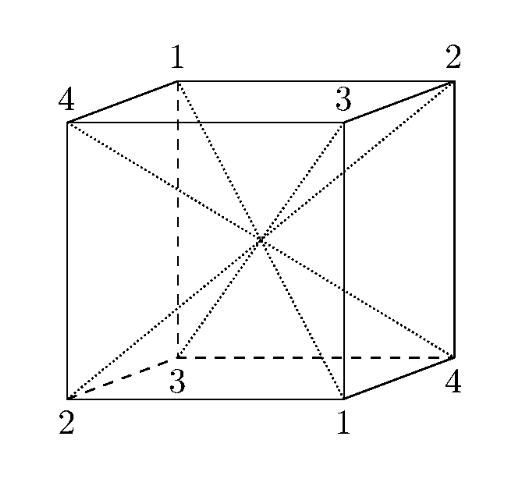
\includegraphics[width=0.5\textwidth]{1.jpg}
            \caption{From \url{https://math.stackexchange.com/questions/751507}.}
            \label{fig:Figure1}
        \end{figure}
        \item Let $G$ be your favorite group with a subgroup $H$ (not necessarily normal). Then $G$ acts by permutation on the set of left cosets $\quotient{G}{H}$ of $H$. This extends linearly to a representation of dimension $[G:H]$, the index of $H$ in $G$.
    \end{enumerate}
\end{example}
\subsection{Isomorphism of Representations}
Certainly, you would want isomorphic representations to have the same field, dimension $n$, and group $G$. So let $\rho_1:G\to\Aut(V_k)$, $\rho_2:G\to\Aut(W_k)$, be two $n$-dimensional representations over $k$. An \textbf{isomorphism of representations} is a vector space isomorphism $f:V_k\xlongrightarrow{\sim}W_k$ that preserves the $G$-action. Intuitively, $f(gv)=gf(v)$ for all $g\in G$, $v\in V$. Precisely
\begin{equation}
    f\left(\rho_1(g)v\right)=\rho_2\left(g\right)f(v)
\end{equation}
for all $g\in G$, $v\in V$.

If we fix bases for $V$ and $W$, then we can think of $f$ as an $n\times n$ matrix, necessarily invertible. Call it $C$. Then $C\rho_1(g)v=\rho_2(g)v$ for all $v\in V$, $g\in G$. Then
\begin{equation}
    \begin{split}
        C\rho_1(g)&=\rho_2(g)C\\
        \Rightarrow\rho_1(g)&=\inv{C}\rho_2(g)C
    \end{split}
\end{equation}
for all $g\in G$. $C$ is just your change of basis matrix! So two $G$-representations on the same vector space are isomorphic if and only if they are the same after a \underline{consistent} change of basis.
\subsection{Group Rings and Modules}
Start with $\q$ (or your favorite commutative ring). Let $G$ be your favorite group, written multiplicatively. Form the \textbf{group ring}, a.k.a. the \textbf{group algebra}:
\begin{equation}
    \begin{split}
        R\coloneqq \q G&=\left\{\sum\limits_{\alpha_g\in G}\alpha_gg\,\middle|\,\alpha_g\in\q\text { zero for all but finitely many }g\in G\right\}\\
        &=\text{ linear combinations of elements of $G$ with coefficients in $\q$.}
    \end{split}
\end{equation}
We just saw $\q G$ as a vector space. So we can \ita{add} elements of $\q G$. But we can also \ita{multiply} them and make it a ring.
\begin{example}
    $\q S_3$ like last time (this time write the rational coefficients on the left). Some sample multiplication:
    \begin{equation}
        \begin{split}
            \left[3e+5(1\,2)\right]\left[(1\,2\,3)-7(2\,3)\right]&=3e(1\,2\,3)-21e(2\,3)+5(1\,2)(1\,2\,3)-35(1\,2)(2\,3)\\
            &=3(1\,2\,3)-21(2\,3)+5(2\,3)-35(1\,2\,3)\\
            &=\boxed{-16(2\,3)-32(1\,2\,3).}
        \end{split}
    \end{equation}
    The multiplicative identity is $1e$. In fact, $\q$ lives inside $\q G$, by identifying $\alpha\in\q$ with $\alpha e\in\q G$. Note that $\q G$ is a commutative ring if and only if $G$ is abelian.
\end{example}
\begin{remark}
    Yes, I know we started with writing coefficients on the right, but when we're dealing with \underline{vector spaces} it actually doesn't matter which side the scalars multiply on (in future terminology, vector spaces over $k$ are $k$-$k$-bimodules where the actions of $k$ on the left and right coincide). So in keeping with practice, we'll write the scalars on the left for vector spaces. Do be careful with the distinction for more general modules, as we'll be dealing with both \underline{left} and \underline{right} modules in this course.
\end{remark}
\section{February 3}
\subsection{Blitz}
Let $G\coloneqq \z_5=\{e,g,g^2,g^3,g^4\}$ with $g^5=e$. In the group ring $R\coloneqq \q G$, let 
\begin{align*}
    a&\coloneqq e-g,&&c\coloneqq e-g^2-g^3\\
    b&\coloneqq e+g+g^2+g^3+g^4,&&d\coloneqq e-g-g^4.
\end{align*}
Compute $ab$ and $cd$.
\subsection{Group Rings}
Let $k$ be a field (or commutative ring), $G$ be a group written multiplicatively. Then the group ring $kG$ is 
\begin{equation}
    \left\{\sum\limits_{g\in G}\alpha_gg\,\middle|\,\alpha_g\in k\text{ nonzero for finitely many }g\right\}.
\end{equation}
\underline{Digression for thrill-seekers}: The blitz produced \underline{zero divisors} and units! Of course, group rings will always have the trivial units $g\inv{g}=1$. But $c$ and $d$ are \ita{nontrivial} units.

Note that $c$ and $d$ relied on \underline{torsion} in $G$, \ita{i.e.}, all elements of $G$ having finite order. In our example, since $G$ itself had finite order, then every element has finite order. This raises interesting questions: suppose $k$ is a domain (like $\q$) and $G$ is \underline{torsion-free} (every non-identity element has infinite order, like $\z$). Can the group ring have
\begin{enumerate}
    \item nontrivial units?
    \item nontrivial zero-divisors?
    \item nilpotent ($r^n=0$) elements besides $r=0$?
\end{enumerate}
\underline{Answers}: Find examples or prove that they don't exist.
\subsection{Group Rings and Representation Theory}
Let $k$ be a field, $G$ a group. Then we have a perfect equivalence:
\begin{equation}
    \{\text{ representations of $G$ over $k$ }\}\xlongleftrightarrow{}\{\text{ left $kG$-modules }\}.
\end{equation}
\begin{itemize}
    \item $\xlongrightarrow{}$: Given a group action of $G$ on $V$, we can make $V$ into a left $kG$-module:
    \begin{equation}
        \left(\sum\limits_{g\in G}\alpha_gg\right)(v)\coloneqq \sum\limits_{g\in G}\alpha_g\rho(g)(v).
    \end{equation}
    \item $\xlongleftarrow{}$: Given a left $kG$-module $V$, note that there is a copy of $k$ inside $kG$ ($\alpha\in k\leftrightarrow\alpha e\in kG$), so $V$ is a $k$-module, that is, a $k$-vector space. So $G$ acts on a $k$-vector space, so we have a group representation.
\end{itemize}
Make this second nature! 
\begin{example}
    \noindent
    \begin{enumerate}
        \item The permutation representation of $S_3$ over $\q$ is now just a module over $R\coloneqq \q S_3$. For example,
        \begin{equation}
            \begin{split}
                \underbrace{\left[5e-2(a\,b)+4(a\,b\,c)\right]}_{r\in R}\underbrace{(2a+6b-c)}_{m\in M}&=10a+30b-5c-4b\\
                &-12a+2c+8b+24c-4a\\
                &=\boxed{-6a+34b+21c}\in M.
            \end{split}
        \end{equation}
        An isomorphism of representations is just an isomorphism of left $kG$-modules: $f:V\xlongrightarrow{\sim}W$ must respect addition and (left) scalar multiplication: 
        \begin{equation}
            f(rv_1+v_2)=rf(v_1)+f(v_2)
        \end{equation}
        for all $v_1,v_2\in V$, $r\in R\coloneqq kG$.
        \item For any field $k$, group $G$, consider the group $R\coloneqq kG$ as a left module $\,_RR$ over itself. Then $\rho(g):h\mapsto gh$. This is exactly the Regular representation.
    \end{enumerate}
\end{example}
\subsection{Operations on Representations: Subrepresentations}
\begin{definition}
    Given a group representation of $G$ on $V$, a \textbf{subrepresentation} is a vector subspace $W\subseteq V$ that is \underline{invariant} under $G$, meaning $gW\subseteq W$ for all $g\in G$ (setwise, not elementwise). Equivalently, $W$ is a left $kG$-submodule of $V$ (it is closed under addition and scalar multiplication from $kG$).
\end{definition}
\begin{definition}
    $V$ is an \textbf{irreducible representation} (\underline{irrep} for short) if it has no nontrivial proper subrepresentations. Equivalently, $V$ is a \underline{simple} left $kG$-module (has no nontrivial proper submodules).
\end{definition}
\begin{example}
    Let $V$ be the permutation representation of $S_3$ over $\q$, which is three-dimensional. We found two subrepresentations:
    \begin{equation}
        \begin{split}
            W&\coloneqq \spank{\q}\{(1,1,1)\}\\
            U&\coloneqq \spank{\q}\{(1,-1,0),(0,-1,1)\}.
        \end{split}
    \end{equation}
    So $V$ is \ita{not} irreducible, but $W$ \ita{is} irreducible, since $\dim_{\q}(W)=1$. How about $U$?
\end{example}
As with the Regular representation, we can look at subrepresentations using matrices. Given a subrepresentation $W\subseteq V$, choose a basis $\{w_1,\dotsc,w_r\}$ of $W$ and then complete it to a basis $\{w_1,\dotsc,w_r,v_{r+1},\dotsc,v_n\}$ of $V$. Then in this basis, every $g\in G$ will correspond to a matrix like
\begin{equation}
    \left[\begin{array}{c c | c c c}
        * & * & * & * & * \\
        * & * & * & * & * \\
        \hline 
        0 & 0 & * & * & * \\
        0 & 0 & * & * & * \\
        0 & 0 & * & * & *
    \end{array}
    \right],
\end{equation}
where the upper left block corresponds to $W\to W$, the upper right block corresponds to elements of $V$ not in $W$ that get sent to $W$, and the lower right block corresponds to elements of $V$ not in $W$ staying outside of $W$. The lower left block must be all zeros, since $gW\subseteq W$.
\begin{example}
    Take the Permutation representation of $S_3$, with $W\subset V$. Start with $(1,1,1)$ to span $W$ and complete it to the basis $\{(1,1,1),(1,0,0),(0,1,0)\}$ for $V$. Then we get
    \begin{equation}
        e\mapsto
        \left[\begin{array}{c | c c}
            1 & 0 & 0 \\
            \hline 
            0 & 1 & 0 \\
            0 & 0 & 1  
        \end{array}
        \right],
        \quad
        (1\,2)\mapsto
        \left[\begin{array}{c | c c}
            1 & 0 & 0 \\
            \hline 
            0 & 0 & 1 \\
            0 & 1 & 0  
        \end{array}
        \right],
        \quad
        (1\,3)\mapsto
        \left[\begin{array}{c | c c}
            1 & 1 & 0 \\
            \hline 
            0 & -1 & 0 \\
            0 & -1 & 1  
        \end{array}
        \right].
    \end{equation}
\end{example}
\section{February 5}
\subsection{Blitz}
In the Permutation representation of $S_3$ with the ordered basis 
\[\{(1,1,1),(1,0,0),(0,1,0)\}\]
(chosen because $W\coloneqq \spank{\q}\{(1,1,1)\}$ is a subrepresentation), find the matrix corresponding to $g\coloneqq (1\,2\,3)\in S_3$.
\subsection{Operations on Representations}
Our story so far: let $k$ be any field, $G$ be any finite group, $R\coloneqq kG$ the group ring. Then we have a perfect correspondence
\begin{equation}
    \begin{split}
        \{\text{ representations of $G$ on $V$ over $k$ }\}&\xlongleftrightarrow{}\{\text{ left $kG$-modules $_{kG}V$ }\}\\
        \{\text{ subrepresentations $\coloneqq$  invariant subspaces }\}&\xlongleftrightarrow{}\{\text{ left $kG$-submodules $_{kG}W$ }\}.
    \end{split}
\end{equation}
We move on to more operations on representations.
\begin{enumerate}
    \setcounter{enumi}{1}
    \item \underline{Quotients}:
    \begin{definition}
        Given a representation $W\subseteq V$, we can define the \textbf{factor (quotient) representation} to be $\quotient{V}{W}$ as a vector space with group action defined by $g(\overline{v})\coloneqq \overline{g(v)}$.
    \end{definition}
    Here comes the usual question: Is it well-defined? Yes, by Homework.

    This definition is trivial in module language: given a left submodule $W\subseteq V$ over $kG$, we can form the usual quotient module $\quotient{V}{W}$.
    \begin{example}
        In the Permutation representation of $S_3$, we have the quotient representation $\quotient{V}{W}$ of dimension 2. 
    \end{example}
    \item \underline{Direct sums}:
    \begin{definition}
        Given two representations of the same group $G$ over the same field $k$, say 
        \begin{equation}
            \begin{split}
                \rho_1&:G\to\Aut(W)\simeq\GL_n(k),\\
                \rho_2&:G\to\Aut(U)\simeq\GL_m(k),
            \end{split}
        \end{equation}
        we can form their \textbf{direct sum}:
        \begin{equation}
            (\rho_1\oplus\rho_2):G\to\Aut(W\oplus U)\simeq \GL_{n+m}(k),
        \end{equation}
        with $G$-action defined by $g(w,u)\coloneqq (g(w),g(u))$. That is, $(\rho_1\oplus\rho_2)(g)(w,u)\coloneqq \left(\rho_1(g)(w),\rho_2(g)(u)\right)$.
    \end{definition}
    If we concatenate bases of $W$ and $U$ to get a basis for $W \oplus U$, then we get nice matrix blocks:
    \begin{equation}
        (\rho_1\oplus\rho_2)(g)=
        \left[\def
        \arraystretch{1.5}\begin{array}{c | c}
            \rho_1(g) & 0  \\
            \hline 
            0 & \rho_2(g)  
        \end{array}\right].
    \end{equation}
    The \underline{fundamental questions} of direct sums is this: given a subrepresentation $W\subseteq V$, does it \underline{split}? That is, is there a \textbf{complementary} subrepresentation $U\subseteq V$ such that $V=W\oplus U$? 
    \begin{example}
        In the Permutation representation of $S_3$, $W$ splits because $V=W\oplus U$ (usually).
    \end{example}
    The matrix formulation of this question is this: given $W\subseteq V$ with matrices of the form 
    \begin{equation}
        \left[\begin{array}{c | c}
            * & *  \\
            \hline 
            0 & *  
        \end{array}\right],
    \end{equation}
    can we reorganize our bases to give us matrices of the form 
    \begin{equation}
        \left[\begin{array}{c | c}
            * & 0  \\
            \hline 
            0 & *  
        \end{array}\right]?
    \end{equation}
    The upper right block vanishing tells us that $U$ does not spill over into $W$. That maintains the fact that in the direct sum $W\oplus U$, $W$ and $U$ do not talk to each other at all (apart from the zero vector). 
    \item \underline{Tensor products}:
    Given $k$-vector spaces $V$ and $W$, we can form the \textbf{tensor product $V\otimes W$}, sometimes written with the subscript $V\otimes_kW$:
    \begin{equation}
        V\otimes W\coloneqq \left\{\sum\limits_{i=1}^n(v_i\otimes w_i)\,\middle|\,v_i\in V,w_i\in W, n\geq1\right\}\bigg/\sim,
    \end{equation}
    where $\sim$ is the set of relations to define \textbf{bilinearity}: 
    \begin{itemize}
        \item $v\otimes(w_1+w_2)=v\otimes w_1+v\otimes w_2$ and $(v_1+v_2)\otimes w=v_1\otimes w+v_2\otimes w$.
        \item $v\alpha\otimes w=v\otimes\alpha w$ for $\alpha\in k$.
    \end{itemize}
    It's useful to write scalars in the middle. Later we'll study tensor products of modules: combine a right module $M_R$ with a left module $_RN$ to get $M\otimes_RN$, and we'll say $mr\otimes n=m\otimes rn$.
    \begin{remark}
        Note that $V\otimes W$ is defined as \ita{sums} of elements of the form $v\otimes w$, for $v\in V$, $w\in W$. Such elements are called \underline{simple tensors}. As it turns out, not every element of $V\otimes W$ is a simple tensor. This fact leads to emergence of entanglement in a system of two spin-$\frac{1}{2}$ particles in Quantum Mechanics!
    \end{remark}
    Let's take bases $\{v_1,\dotsc,v_n\}$, $\{w_1,\dotsc,w_m\}$ for $V$ and $W$. Then $V\otimes W$ has basis 
    \begin{equation}
        \{v_1\otimes w_1,v_1\otimes w_2,\dotsc,v_n\otimes w_m\}=\{v_i\otimes w_j\mid 1\leq i\leq n,1\leq j\leq m\},
    \end{equation}
    so it has dimension $nm$. Notice how the dimensions \ita{multiply} instead of adding, as in the direct sum.
    \begin{definition}
        We define the \textbf{tensor representation}
        \begin{equation}
            (\rho_1\otimes\rho_2):G\to\Aut(V\otimes W)\simeq\GL_{mn}(k)
        \end{equation}
        by $g(v\otimes w)\coloneqq g(v)\otimes g(w)$, that is, $(\rho_1\otimes\rho_2)(g)(v\otimes w)\coloneqq \rho_1(g)(v)\otimes\rho_2(g)(w)$.
    \end{definition}
    It's best to define the matrix formulation in terms of an example. Suppose 
    \begin{equation}
        \begin{split}
            \rho_1(g)&=A=
            \begin{bmatrix}
                a_{11} & a_{12} \\[0.3em]
                a_{21} & a_{22}
            \end{bmatrix},\\
            \rho_2(g)&=B=
            \begin{bmatrix}
                b_{11} & b_{12} & b_{13} \\[0.3em]
                b_{21} & b_{22} & b_{23} \\[0.3em]
                b_{31} & b_{32} & b_{33}
            \end{bmatrix},
        \end{split}
    \end{equation}
    then $(\rho_1\otimes\rho_2)(g)=A\otimes B$ can be defined as either 
    \begin{equation}
        \def\arraystretch{1.5}
        \left[\begin{array}{c | c}
            a_{11}B & a_{12}B  \\
            \hline 
            a_{21}B & a_{22}B  
        \end{array}\right]
    \end{equation}
    or 
    \begin{equation}
        \def\arraystretch{1.5}
        \left[\begin{array}{c | c | c}
            Ab_{11} & Ab_{12} & Ab_{13} \\
            \hline
            Ab_{21} & Ab_{22} & Ab_{23} \\
            \hline
            Ab_{31} & Ab_{32} & Ab_{33}
        \end{array}\right],
    \end{equation}
    depending on which way you order the big basis for $V\otimes W$ (horizontally or vertically).
    \begin{remark}
        Warning! Many references, including ours, give the tensor product of representation of two \ita{different} groups: given $\rho:G\to\Aut(V)$, $\sigma:H\to\Aut(W)$, they form $(\rho\otimes\sigma):G\times H\to\Aut(V\otimes W)$ by $(\rho\otimes\sigma)(g,h):v\otimes w\mapsto\rho(g)(v)\otimes\sigma(h)(w)$. If we applied this definition to our convention, we would be getting $(\rho_1\otimes\rho_2):G\times G\to\Aut(V\otimes W)$ instead. However, we \ita{can} reconcile these two conflicting definitions by insisting that ours restrict to the isomorphic copy of $G$ in $G\times G$. 
    \end{remark}
\end{enumerate}
\section{February 10}
\subsection{Blitz}
Define 
\[A\coloneqq 
\begin{bmatrix}
    1 & 2 \\
    3 & 4
\end{bmatrix},
\qquad
B\coloneqq 
\begin{bmatrix}
    1 & 2 & 3 \\
    4 & 5 & 6 \\
    7 & 8 & 9
\end{bmatrix}.
\]
Compute $A\otimes B$. As a bonus, why would we not encounter $A$ or $B$ as $\rho(g)$ in our journey together? (Two answers possible.) 
\subsection{Exact Sequences}
\begin{remark}
    Oh boy, here we go again. Lemme cue up ``The Sound of Silence'' by Simon $\&$ Garfunkel... (listen here: \url{https://www.youtube.com/watch?v=f7McpVPlidc}).
\end{remark}
\begin{definition}
    Consider a sequence of $R$-modules and homomorphisms:
    \begin{equation}
        \dotsb \xlongrightarrow{\phi_{n-2}}A_{n-1}\xlongrightarrow{\phi_{n-1}}A_n\xlongrightarrow{\phi_n} A_{n+1}\xlongrightarrow{\phi_{n+1}}\dotsb
    \end{equation}
    where $\phi_n:A_n\to A_{n+1}$, where $n$ may possibly range over all of $\z$. The sequence is \textbf{exact} at every stage if $\im\phi_{n-1}=\ker\phi_n$.
    A \textbf{short exact sequence} is one of the following form:
    \begin{equation}
        \{0\}\xlongrightarrow{} A\xlongrightarrow{\phi}B\xlongrightarrow{\psi}C\xlongrightarrow{}\{0\}
    \end{equation}
    The homomorphisms are $\phi:A\to B$ and $\psi:B\to C$. The end maps have only one possible homomorphism: the inclusion map and the constant map, respectively.
\end{definition}
Let's unpack this definition:
\begin{enumerate}
    \item Exactness at $A$ means $\ker\phi=\im(\{0\})=\{0\}$, so this means precisely that \underline{$\phi$ is injective}. So $\im\phi\simeq A$.
    \item Exactness at $C$ means $\im\psi=\ker0=C$, so this means precisely that \underline{$\psi$ is surjective}.
    \item Exactness at $B$ means $\im\phi=\ker\psi$. So by the First Isomorphism Theorem (for modules), we get $\quotient{B}{\ker\psi}\simeq\im\psi=C$, and $\quotient{B}{\im\phi}=\quotient{B}{(\text{something isomorphic to }A)}$.
\end{enumerate}
\underline{Intuition (part 1)}: A short exact sequence tells you that in some sense, $B$ is \ita{composed} of copies of $A$ and $C$: $B$ has ``$A$'' as a submodule, with factor module ``$C$.'' Conversely, given a module $B$ with a submodule $A\subseteq B$, you can build a short exact sequence using the natural maps
\begin{equation}
    \{0\}\xlongrightarrow{} A\xlongrightarrow{\Id}B\xlongrightarrow{\pi}C\coloneqq \quotient{B}{A}\xlongrightarrow{}\{0\}.
\end{equation}
\begin{theorem}[Splitting Headache!]
    Let 
    \begin{equation}
        \{0\}\xlongrightarrow{} A\xlongrightarrow{\phi}B\xlongrightarrow{\psi}C\xlongrightarrow{}\{0\}
    \end{equation}
    be a short exact sequence. Then the following are equivalent:
    \begin{enumerate}
        \item There exists a homomorphism $f:B\to A$ such that $f\circ\phi=\Id_A$.
        \item There exists a homomorphism $g:C\to B$ such that $\psi\circ g=\Id_C$.
        \item $B=\im\phi\oplus T$ for some submodule $T\subseteq B$. (Note that necessarily, we would have $T\simeq\quotient{B}{\im\phi}\simeq C$, so $B\simeq A\oplus C$). 
    \end{enumerate}
    If these conditions are true, then we say the sequence \textbf{splits}. Here's a diagram that sums up what's going on.
    \begin{equation}
        \begin{tikzcd}
            \{0\}\arrow[r] & A\arrow[r,"\Id_A"]  & A\oplus C\arrow[r,"\pi_C"] & C\arrow[r] & \{0\}\\
            \{0\}\arrow[r] &  A\arrow[r,"\phi"]\arrow[r,dashleftarrow, "\exists f", bend right=60] & B\arrow[r,"\psi"]\arrow[u,dashrightarrow, "\exists\Phi"]\arrow[r,dashleftarrow, "\exists g", bend right=60] & C\arrow[r] & \{0\}
        \end{tikzcd}
    \end{equation}
\end{theorem}
\begin{proof}
    Homework.
\end{proof}
\begin{example}
    The sequence 
    \begin{equation}
        \{0\}\xlongrightarrow{} \z_2\xlongrightarrow{1\mapsto2}\z_4\xlongrightarrow{1\mapsto1}\z_2\xlongrightarrow{}\{0\}
    \end{equation}
    does \ita{not} split. Why? We can check all three equivalent conditions: no homomorphism $f:\z_4\to\z_2$ or $g:\z_2\to\z_4$ works, but the quickest way is to realize this is simply because $\z_4\not\simeq\z_2\oplus\z_2$!
\end{example}
\noindent\underline{Intuition (part 2)}: A \underline{split} short exact sequence tells you that $B$ is composed of \ita{separable} (no, not dense countable subset!) copies of $A$ and $C$. $K_4$ is composed of two separate $\z_2$'s in a way that $\z_4$ is not.
\subsection{Maschke's Theorem}
\begin{theorem}[Maschke's Theorem]
    Let $V$ be a finite-dimensional representation of $G$ with a subrepresentation $W\subseteq V$. Assume that $\mathrm{char}k\nmid|G|$. Then $W$ has a \underline{complementary} subrepresentation $U\subseteq V$, meaning $V=W\oplus U$.
\end{theorem}
\begin{remark}
    We will build our church upon this rock!
\end{remark}
\noindent\underline{Consequences of Maschke}: Assume $\mathrm{char}k\nmid|G|$.
\begin{enumerate}
    \item Every subrepresentation splits.
    \item Every finite-dimensional representation decomposes into a finite direct sum of irreducibles:
    \begin{equation}
        V=W_1\oplus\dotsb\oplus W_r,
    \end{equation}
    with $W_i$ irreducible.
    \item In ring language, this says $kG$ is a \underline{semisimple} ring. In fact, we have a complete structure theory for semisimple rings and their modules, as we'll learn anon.
\end{enumerate}
(So if $\mathrm{char}k=0$, like with $\q$, $\real$, and $\cx$, all of this is true for all finite groups!)
\begin{proof}
    Start with your subrepresentation $W\subseteq V$. Forget the group action and as \underline{vector} \underline{spaces only}, find a direct complement $V=W\oplus T$ (for \underline{vector spaces} it is easy to find complements: take a basis $\{w_1,\dotsc,w_r\}$ for $W$ and complete it to a basis $\{w_1,\dotsc,w_r,t_{r+1},\dotsc,t_n\}$ for $V$. Then Let $T\coloneqq \mathrm{span}_k\{t_{r+1},\dotsc,t_n\}$). But $T$ almost certainly won't be $G$-invariant. Define the projection map $f:V\to W$ by this decomposition: $f(w+t)\coloneqq w$. Again, note that $f$ is a \underline{vector space} map only; it probably does \ita{not} respect the $G$-action. Smooth out $f$ by ``averaging:'' define a new map 
    \begin{equation}
        \overline{f}(v)\coloneqq \frac{1}{|G|}\sum\limits_{g\in G}gf\inv{g}(v).
    \end{equation}
    (Technically, we should write $\overline{f}\coloneqq \frac{1}{|G|}\sum\limits_{g\in G}\rho(g)\circ f\circ\rho(\inv{g})$). More next time!
\end{proof}
\section{February 12}
\subsection{Blitz}
Show in two ways that the short exact sequence of abelian groups
\[\{0\}\xlongrightarrow{}\underbrace{\z_2}_{=A}\xlongrightarrow{\phi:1\mapsto3}\underbrace{\z_6}_{=B}\xlongrightarrow{\psi:t\mapsto1}\underbrace{\z_3}_{=C}\xlongrightarrow{}\{0\}\]
does \ita{split}.
\begin{enumerate}
    \item Give me a homomorphism $f:B\to A$ such that $f\circ\phi=\Id_A$.
    \item Give me a homomorphism $g:C\to B$ such that $\psi\circ g=\Id_C$.
\end{enumerate}
\subsection{Finishing Up Maschke's Theorem}
Recall \underline{Maschke's Theorem}: Let $V$ be a finite-dimensional representation with a subrepresentation $W\subseteq V$. Assume $\mathrm{char}k\nmid|G|$. Then $W$ splits: there is a subrepresentation $U$ such that $V=W\oplus U$.
\begin{proof}
    Find a vector space direct complement $V=W\oplus T$ (by completing a basis). Project $f:V\to W$ as vector spaces, probably not respecting the group action! To overcome this, we average $f$ out: define
    \begin{equation}
        \overline{f}(v)\coloneqq \frac{1}{|G|}\sum\limits_{g\in G}gf\inv{g}(v).
    \end{equation}
    We need 3 more steps:
    \begin{enumerate}
        \setcounter{enumi}{4}
        \item For all $v\in V$, we have $\overline{f}(v)\in W$. So $\overline{f}$ maps $V$ to $W$.
        \item $\overline{f}$ is the identity on $W$.
        \item This is the key step: $\overline{f}$ respects not just the vector space structure, but also the \underline{$G$-action}, that is, for all $v\in V$ and $h\in G$, we have $\overline{f}(hv)=h\overline{f}(v)$.
    \end{enumerate}
    So we have an exact sequence of \underline{$kG$-modules}:
    \begin{equation}
        \begin{tikzcd}
            \{0\}\arrow[r] & W\arrow[r,"\Id_W"]\arrow[r,dashleftarrow, "\overline{f}"', bend right=60]  & V\arrow[r,"\pi",twoheadrightarrow] & \quotient{V}{W}\arrow[r] & \{0\}
        \end{tikzcd}
    \end{equation}
    Note that $\overline{f}\circ\Id_W=\Id_W$, so we have split the sequence! By Splitting Headache, we get $V=W\oplus U$ \underline{as $kG$-modules}, so $U$ is the complementary subrepresentation we sought.
\end{proof}
\subsection{Results of Maschke}
With Maschke in our toolkit, we can deduce several results. First, let's build up some lemmas:
\begin{lemma}[Schur's Lemma]
    Let $R$ be a ring, and let $_RM$ and $_RN$ be \underline{simple} left $R$-modules. Then any homomorphism $f:M\to N$ is either $0$ or an isomorphism.
\end{lemma}
\begin{proof}
    Homework.
\end{proof}
\begin{corollary}[Division Ring Corollary]
    Let $_RM$ be a simple left $R$-module. Then $\End(_RM)$ is a division ring.
\end{corollary}
As a refresher, here's a definition of division ring.
\begin{definition}
    A \textbf{division ring} is a ring in which every nonzero element has an inverse.
\end{definition}
In other words, a division ring is a field except that it might not be commutative. 
\begin{remark}
    In fact, the term ``field'' used to refer to division rings in general, and what we call fields now, \ita{i.e.}, commutative division rings, were called ``commutative fields.'' Another older terminology for noncommutative division rings is ``skew field.''
\end{remark}
\begin{example}
    \noindent
    \begin{enumerate}
        \item Every field qualifies.
        \item The ring of real quaternions is a division ring:
        \begin{equation}
            \mathbb{H}\coloneqq \{a+bi+cj+dk\mid a,b,c,d\in\real\}.
        \end{equation}
        Restricting the coefficients to a proper subring of $\real$, say $\q$, gives a subring of $\mathbb{H}$ which is also a division ring.
    \end{enumerate}
\end{example}
\begin{corollary}[Schur Endomorphism Corollary]
    Let $G$ be a group and $V$ a simple $\cx G$-module, that is, an irreducible $G$ representation. Then $\End(_{\cx G}V)\simeq\cx$, that is, the only kind of endomorphism is multiplication from $\cx$.
\end{corollary}
This also works with $\cx$ replaced by any \underline{algebraically closed} field.
\begin{proof}
    Take $f\in\End(_{\cx G}V)$. Considering $f$ just as a vector space homomorphism, that is, as a linear transformation, $f$ must have an eigenvalue $\lambda \in \cx$ with a nonzero eigenvector $v$ (this uses $\cx$ being algebraically closed!). Now, consider the homomorphism $(f-\lambda)\in\End(_{\cx G}V)$. We know $(f-\lambda)v=0$, so $f-\lambda$ is not invertible. So by Schur's lemma, we must have $f-\lambda=0$, so $f$ is just multiplication by $\lambda$.
\end{proof}
\begin{corollary}[Abelian Corollary]
    Any complex irreducible representation of an \underline{abelian} group is one-dimensional.
\end{corollary}
\begin{proof}
    Let $G$ be abelian, let $R\coloneqq \cx G$, and let $V$ be a simple $R$-module. Choose any nonzero $v\in V$. For any other $w\in V$, simplicity gives us $rv=w$ for some $r\in R$ (otherwise $Rv\coloneqq \{rv\mid r\in R\}$ is a proper submodule of $V$). Suppose 
    \begin{equation}
        \left(\sum\limits_{g\in G}\alpha_gg\right)v=w,
    \end{equation}
    where $\alpha_g\in\cx$. Each $g\in G$ commutes with the rest of $G$, so each $g\in\End(_RV)$. By the Schur Endomorphism Corollary (SEC), each $g$ acts by complex multiplication, say by some $\lambda_g\in\cx$. So 
    \begin{equation}
        w=\left(\sum\limits_{g\in G}\alpha_gg\right)v=\underbrace{\left(\sum\limits_{g\in G}\alpha_g\lambda_g\right)}_{\in\cx!}v,
    \end{equation}
    and $w$ is a complex multiple of $v$. We chose $w\in V$ arbitrarily, so $V=\mathrm{span}_{\cx}\{v\}$.
\end{proof}
\section{February 17}
\subsection{Blitz}
Given two representations $W\subseteq V$ of the group $A_4$ over a field $k$, we can guarantee that $W$ splits from $V$ if (choose any that are correct):
\begin{multicols}{3}
    \begin{enumerate}[A)]
        \item $k=\z_2$
        \item $k=\z_3$
        \item $k=\z_5$
        \item $k=\q$
        \item $k=\cx$.
    \end{enumerate}
\end{multicols}
\subsection{Semisimple Modules}
Maschke tells us that subrepresentations have direct complements. We'll exploit this to find a powerful structure theory for $kG$ and its modules, a.k.a., representations of $G$ over $k$.

Throughout, let $R$ be a ring (our rings include 1) and $_RM$ be a left $R$-module.
\begin{definition}
    Recall that $_RM$ is \underline{simple} if it is nonzero and has no proper nontrivial submodules. This is true if and only if $M\neq0$ and any nonzero $m\in M$ \textbf{generates} $M$, meaning $Rm=M$.
\end{definition}
\begin{example}
    \noindent
    \begin{enumerate}
        \item A vector space over a field is simple if and only if it is one dimensional.
        \item For $n\in\z^+$, the abelian group $\z_n=\quotient{\z}{n\z}$ is simple as a $\z$-module if and only if $n$ is prime.
    \end{enumerate}
\end{example}
\begin{definition}
    $_RM$ is \textbf{semisimple} if every submodule $_RN\subseteq\,_RM$ has a direct complement, that is, there exists a submodule $_RK$ such that $N\oplus K=M$.
\end{definition}
Note that the zero module \ita{is} semisimple.
\begin{example}
    \noindent
    \begin{enumerate}
        \item Simple implies semisimple, vacuously.
        \item Any vector space over any field is semisimple, by extending a basis.
    \end{enumerate}
\end{example}
\begin{lemma}[Simple Lemma]
    Any nonzero semisimple module contains a simple submodule.
\end{lemma}
\begin{proof}
    Let $0\neq\,_RM$ be semisimple, and let $0\neq m\in M$. If the submodule $Rm$ is simple, then we are done. If not, then by Homework (submodules of semisimple modules are semisimple), $Rm$ is semisimple. Now use Zorn's Lemma to find a submodule $N\subset Rm$ maximal with respect to the property that $m\notin N$. By semisimplicity of $Rm$, we can find a direct complement $N\oplus K=Rm$. We claim that $_RK$ is simple. If not, then $K$ has a proper nontrivial submodule $0\neq L\subsetneq K$. Then $(N\oplus L)\supsetneq N$, so $m\in N\oplus L$. Say $m=n+l$ with $n\in N$, $l\in L\subsetneq K$. Then for anhy $k\in K\subseteq Rm$, we have $k=rm$ for some $r\in R$, so $k=rn+rl$. But then $k-rl=rn\in K\cap N$, so $k=rl\in L$. So $K\subseteq L$, contradicting $L\subsetneq K$. So $_RK$ is a simple submodule, and so $_RM$ has a simple submodule.
\end{proof}
\begin{remark}
    For such a name as ``Simple Lemma,'' this was not a simple proof at all!
\end{remark}
\noindent
\underline{Note that for unchoosy representation theorists}: the rings we'll apply this to are group rings $kG$. The modules $_{kG}M$ will be $k$-vector spaces, and they will be finite-dimensional. In such a case, we wouldn't need the Simple lemma, because if $M_0\coloneqq M$ is not simple, then it has a (nontrivial) proper submodule $M_1$. If $M_1$ is not simple, then we find $M_2\subsetneq M_1\subsetneq M_0$. Just by considering the $M_i$'s as $k$-vector spaces, the dimension drops each time, so we have to terminate at a simple submodule.
\begin{definition}
    Let $\{M_{\alpha}\}_{\alpha}$ be a set of submodules of $_RM$. 
    \begin{enumerate}
        \item We say
        \begin{equation}
            M=\sum\limits_{\alpha\in A}M_{\alpha}
        \end{equation}
        if every $m\in M$ can be written as a (finite) sum $m=m_1+\dotsb+m_n$ with $m_i\in M_i$.
        \item We say 
        \begin{equation}
            M=\bigoplus\limits_{\alpha\in A}M_{\alpha}
        \end{equation}
        if $M=\sum\limits_{\alpha\in A}M_{\alpha}$ and the sum is \textbf{direct}, meaning $m_1+\dotsb+m_n=0$ with $m_i\in M_i$ implies that all $m_i=0$. Equivalently, for each $\alpha\in A$, we have 
        \begin{equation}
            M_{\alpha}\cap\sum\limits_{
            \substack{
                \beta\in A \\
                \beta\neq\alpha
            }}
            M_{\beta}=0.
        \end{equation}
    \end{enumerate}
\end{definition}
\begin{theorem}[Semisimple Module Characterization]
    The following are equivalent:
    \begin{enumerate}
        \item $_RM$ is semisimple.
        \item $_RM=M=\sum\limits_{\alpha\in A}M_{\alpha}$ for a set of simple submodules $_RM_{\alpha}$.
        \item $_RM=M=\bigoplus\limits_{\alpha\in A}M_{\alpha}$ for a set of simple submodules $_RM_{\alpha}$.
    \end{enumerate}
\end{theorem}
Note that the zero module, which is semisimple but not simple, is the empty sum of simple modules.
\begin{proof}
    \noindent
    \begin{itemize}
        \item $1\implies3$: Use Zorn's Lemma to find a maximal direct sum of simple submodules $N=\bigoplus\limits_{\alpha\in A}M_{\alpha}\subseteq M$. We claim that $N=M$. If $N\subsetneq M$, then by semisimplicity, we can find a complement $N\oplus K=M$. $K$ is semisimple by Homework, so $K$ contains a simple submodule by the Simple lemma. Call that submodule $_RT\subseteq\,_RK$. But then $N\subsetneq N\oplus T=\left(\bigoplus\limits_{\alpha\in A}M_{\alpha}\right)\oplus T$, contradicting the maximality of $N$. So $N=M=\bigoplus\limits_{\alpha\in A}M_{\alpha}$, proving 3.
        \item $3\implies2$: a fortiori. It doesn't get any easier than this!
        \item $2\implies1$: Next time!
    \end{itemize}
\end{proof}
\section{February 19}
\subsection{Blitz}
$\z_4$ is / is not a simple $\z$-module, and it is / is not a semisimple $\z$-module.
\subsection{Semisimple Modules (cont'd)}
Recall the following definitions:
\begin{itemize}
    \item $_RM$ is \underline{simple} if it is nonzero and has no proper nontrivial representations
    \item $_RM$ is \underline{semisimple} if every submodule $_RN\subseteq\,_RM$ splits: $N\oplus K=M$.
\end{itemize}
\noindent \underline{Semisimple module characterization}: The following are equivalent:
\begin{enumerate}
    \item $_RM$ is semisimple.
    \item $_RM=M=\sum\limits_{\alpha\in A}M_{\alpha}$ for a set of simple submodules $_RM_{\alpha}$.
    \item $_RM=M=\bigoplus\limits_{\alpha\in A}M_{\alpha}$ for a set of simple submodules $_RM_{\alpha}$.
\end{enumerate}
\begin{proof}
$2\implies1$: Let's take a submodule $_RN\subseteq\,_RM$ and find a direct complement. Given $M=\sum\limits_{\alpha\in A}M_{\alpha}$, consider elements $B\subseteq A$ that satisfy two properties:
\begin{enumerate}[(a)]
    \item The sum $\sum\limits_{\alpha\in B}M_{\alpha}$ is direct, and 
    \item $N\cap\left(\sum\limits_{\alpha\in B}M_{\alpha}\right)=0$.
\end{enumerate}
For Homework, you will show that Zorn's Lemma applies to such subsets. Therefore, we can find a maximal subset $B\subseteq A$ satisfying the properties. Define $K\coloneqq \sum\limits_{\alpha\in B}M_{\alpha}$. Then the sum $N+K$ is direct, so we need only show that $M\subseteq(N+K)$. To do this, it suffices to show that any $M_{\alpha}\subseteq(N+K)$. But because $M_{\alpha}$ is simple, if $M_{\alpha}\not\subset(N+K)$, then $M_{\alpha}\cap(N+K)=0$. But then we could adjoin $\alpha$ to $B$ and still satisfy the two properties, contradicting maximality of $B$. Therefore $N+K=M$, and we have our direct complement.
\end{proof}
\subsection{Semisimple Rings}
\begin{definition}
    If the left $R$-module $_RR$ is a semisimple module as a module, then we say $R$ is a \textbf{semisimple ring}.
\end{definition}
Some notes:
\begin{enumerate}
    \item Technically, we should say $R$ is a \underline{left semisimple} ring and define \underline{right semisimple} via the right module $R_R$. But it turns out that the two properties are equivalent (unlike other ring-theoretic properties like noetherian, artinian, \ita{etc}.)
    \item Considering $R$ as a left module over itself, submodules are precisely left ideals. So $R$ being semisimple means precisely that every left ideal $_RI\subseteq\,_RR$ has a direct complement left ideal $_RJ\subseteq\,_RR$ such that $I\oplus J=R$.
    \item Beware ``simple rings.'' (A \textbf{simple ring} has no nontrivial proper \underline{two-sided} ideals. But that's a very weak constraint, and ``simple'' rings can be savage beasts. Semisimple rings are fluffy kittens $\dotsc$)
\end{enumerate}
\begin{remark}
    An example of a simple ring is $\m_n(R)$ for a unital ring $R$. Also, a simple ring may not be semisimple! We will never use the term ``simple ring'' ever again in this class, so when we say simple, always think simple module.
\end{remark}
\underline{Wedderburn-Artin Theory}: For now, let $R$ be a semisimple ring. So by our characterization, $_RR=\bigoplus\limits_{\alpha\in A}\,_RL_{\alpha}$, where the $_RL_{\alpha}$'s are simple left ideals. By Homework, we have $_RR=\bigoplus\limits_{i=1}^nL_i$, where the $L_i$'s are simple left ideals. Organize the $L_i$'s by isomorphism type as simple left modules and reindex them if necessary:
\begin{equation}
    _RR=\Big(L_{11}\oplus\dotsb L_{1n_1}\Big)\oplus\dotsb\oplus\Big(L_{t1}\oplus\dotsb\oplus L_{tn_{t}}\Big)
\end{equation}
where $L_{ik}\simeq L_{i\ell}$ and $L_{ik}\not\simeq L_{j\ell}$ for $i\neq j$. More concisely,
\begin{equation}
    _RR\simeq n_1L_1\oplus\dotsb\oplus n_tL_t
\end{equation}
with $L_i\not\simeq L_j$. Now take endomorphism rings
\begin{equation}
    R\underbrace{\simeq}_{\text{by Homework past!}}\End(_RR)\simeq\End(n_1L_1\oplus\dotsb\oplus n_tL_t).
\end{equation}
Consider the RHS. Any endomorphism $f\in\mathrm{RHS}$ is now mapping lots of bits and pieces to lots of bits of pieces, so $f$ decomposes into block matrix form:
\begin{equation}
    \left[\def\arraystretch{1.5}
    \begin{array}{c | c | c | c}
        f_{11} & f_{12} & \cdots & f_{1t} \\
        \hline
        f_{21} & f_{22} & \cdots & f_{2t} \\
        \hline 
        \vdots & \vdots & \ddots & \vdots \\
        \hline
        f_{t1} & f_{2t} & \cdots & f_{tt}
    \end{array}
    \right]
    \left[\def\arraystretch{1.5}
    \begin{array}{c}
        n_1L_1 \\
        \hline
        n_2L_2 \\
        \hline 
        \vdots \\
        \hline
        n_tL_t
    \end{array}
    \right]
    \xlongrightarrow{}
    \left[\def\arraystretch{1.5}
    \begin{array}{c}
        n_1L_1 \\
        \hline
        n_2L_2 \\
        \hline 
        \vdots \\
        \hline
        n_tL_t
    \end{array}
    \right].
\end{equation}
Here, $f_{ij}$ maps the block of $n_jL_j$ to the block $n_iL_i$, so each $f_{ij}\in\m_{n_i\times n_j}\left(\Hom_R(L_j,L_i)\right)$. But what is $\Hom_R(L_j,L_i)$? Remember that each $L_i$ is a \underline{simple} module. So if $j\neq i$, $\Hom_R(L_i,L_j)=0$ by Schur's lemma, and if $j=i$, then $\Hom_R(L_i,L_i)=\End(_RL_i)$ is a division ring by the Division ring corollary. Define the division ring $D_i\coloneqq \End(_RL_i)$. Then $f_{ij}=0$ for all $i\neq j$, and $f_{ii}\in\m_{n_i}(D_i)$:
\begin{equation}
    f =  
    \left[\def\arraystretch{1.5}
    \begin{array}{c | c | c | c}
        \m_{n_1}(D_1) & 0 & \cdots & 0 \\
        \hline
        0 & \m_{n_2}(D_2) & \cdots & 0 \\
        \hline 
        \vdots & \vdots & \ddots & \vdots \\
        \hline
        0 & 0 & \cdots & \m_{n_t}(D_t)
    \end{array}
    \right].
\end{equation}
So 
\begin{equation}
    R\simeq\End(_RR)\simeq\boxed{\m_{n_1}(D_1)\times\dotsb\times\m_{n_t}(D_t).}
\end{equation}
\begin{theorem}[Wedderburn-Artin Decomposition]
    Let $R$ be a semisimple ring. Then $R$ is (isomorphic to) a finite direct product of matrix rings over division rings.
\end{theorem}
\section{February 24}
\subsection{Blitz}
When we're considering a ring $R$ as a left module $_RR$ over itself, a submodule of $_RR$ is precisely a ( ) of the ring.
\subsection{Modules over Semisimple Rings}
\underline{Wedderburn-Artin}: Let $R$ be a semisimple (any \underline{left module} has a direct complement). Then $R$ is a direct product of matrix rings over division rings:
\begin{equation}
    \boxed{R \simeq \m_{n_1}(D_1) \times \dotsb \times \m_{n_t}(D_t).}
\end{equation}
\underline{Uniqueness (which we won't prove)}: The $n_i$'s and $D_i$'s are uniquely determined (up to isomorphism of the $D_i$'s and permutation of the $i$'s).
\begin{remark}
    What are some actual examples of semisimple rings? Well, by Wedderburn-Artin, $\m_3(\real)$. Also, any division ring $D$ counts, since all of its ideals have direct complements: $D = D \oplus \setb{ 0 }$. However, many of our familiar rings from MATH 540 don't count: take $R \coloneqq  \z$. Then as $\z$ is a PID, all of its ideals are principal. Then as $nm \in n\z \cap m\z$, no nonzero ideals have direct complements, and so $\z$ is not semisimple. 
\end{remark}
Our next goal is to generalize this result:
\begin{equation}
    \text{Wedderburn-Artin} \implies \text{simple modules} \implies \text{all modules}.
\end{equation}
By Homework, if $M$ is a \underline{simple} module over a product ring $R_1 \times \dotsb \times R_n$, then for some $i$, we have that $M$ is a simple module over $R_i$, and $R_jM = 0$ for all $j \in \setb{1 , \dotsc , \hat{i} , \dotsc , n}$. So to describe simple modules over semisimple rings, we just need to understand simple modules over a single Wedderburn component $\m_n(D)$.
\begin{remark}
    What does $\setb{1 , \dotsc , \hat{i} , \dotsc , n}$ mean? It means $\oneton{n} \setminus \setb{ i }$; the hat denotes that $i$ is excluded from the set, and is called a ``tarnhelm.'' The terminology comes from Wagner's Ring Cycle: the Tarnhelm is a magic helmet that Alberich uses in \ita{Das Rheingold} to turn invisible. This lore is courtesy of Dr. Blair.
\end{remark}
\begin{theorem}
    Let $R \coloneqq  \m_n(D)$, where $D$ is a division ring. Let $_RM$ be a left $R$-module over $n \times 1$ column vectors over $D$. Then $_RM$ is simple and $_RR \simeq n\left(_RM\right)$ as left $R$-modules.
\end{theorem}
\begin{proof}
    Homework.
\end{proof}
\begin{remark}
    By $n\left(_RM\right)$, we mean $\bigoplus\limits_{i=1}^n \left(_RM\right)_i$. We write it additively since we're thinking of these modules additively.
\end{remark}
We show that $_RM$ is the \ita{unique} simple left module. First, we need to build up some machinery.
\begin{definition}
    A \textbf{composition series} for $M$ is a finite sequence of submodules
    \begin{equation}
        0 = M_0 \subset M_1 \subset \dotsb \subset M_n = M
    \end{equation}
    such that each factor module $\quotient{ M_{i+1} }{ M_i }$ is simple. These are called the \textbf{composition factors} of $M$.
\end{definition}
Not all modules have composition series. But when they do, the factors are unique.
\begin{theorem}[Refinement Theorem]
    Suppose $_RM$ has a composition series. Then any increasing series of submodules of $M$ can be refined into a composition series. 
\end{theorem}
This means we can insert extra terms into the series to make it a composition series.
\begin{theorem}[Jordan-H\"older Theorem]
    Any two composition series of $_RM$ are equivalent, meaning they have the same number of composition factors, and after a permutation, the factors are isomorphic.
\end{theorem}
\begin{example}
    Let's find two series for the $\z$-module $M \coloneqq  \z_6$:
    \begin{equation}
        \begin{tikzcd}
            0 \arrow[r,symbol=\subset] \arrow[r,dash, "\mathbb{Z}_3"', bend right=60] & \{0 , 2 , 4\} \arrow[r,symbol=\subset] \arrow[r,dash, "\mathbb{Z}_2"', bend right=60] & \z_6 \\
            0 \arrow[r,symbol=\subset] \arrow[r,dash, "\mathbb{Z}_2"', bend right=60] & \{0 , 3\} \arrow[r,symbol=\subset] \arrow[r,dash, "\mathbb{Z}_3"', bend right=60] & \z_6
        \end{tikzcd}
    \end{equation}
\end{example}
For the ring $R \coloneqq  \m_n(D)$, we have a composition series for $_RR$:
\begin{equation}
    0 = M_0 \subset M_1 \subset M_2 \subset \dotsb \subset M_n \coloneqq  R,
\end{equation}
where $M_i$ is the direct sum of the first $i$ copies of $M$. Then 
\begin{equation}
    R = \underbrace{
        \underbrace{
            \underbrace{
                \underbrace{ M }_{ =: M_1 } \oplus M 
                }_{ =: M_2 }
                \oplus M
            }_{ =: M_4 }
            \oplus \dotsb \oplus M
        }_{ =: M_n }
\end{equation}
\begin{example}
    If $R \coloneqq  \m_3(\real)$, then 
    \begin{equation}
        M_1 = 
        \left \{
            \left [
                \begin{array}{c | c | c}
                    \ast & 0 & 0 \\
                    \ast & 0 & 0 \\
                    \ast & 0 & 0  
                \end{array}
            \right ]
        \right \}
        , \quad
        M_2 = 
        \left \{
            \left [
                \begin{array}{c | c | c}
                    \ast & \ast & 0 \\
                    \ast & \ast & 0 \\
                    \ast & \ast & 0  
                \end{array}
            \right ]
        \right \}
        , \quad
        M_3 = 
        \left \{
            \left [
                \begin{array}{c | c | c}
                    \ast & \ast & \ast \\
                    \ast & \ast & \ast \\
                    \ast & \ast & \ast  
                \end{array}
            \right ]
        \right \}
    \end{equation}
\end{example}
\noindent
\underline{Uniqueness of simple modules}: Let $_RP$ be any other simple left $R$-module. Let $0 \neq p \in P$. Then $Rp = P$ because $P$ is simple, so we have a surjective homomorphism of left $R$-modules $R \to P$, $r \mapsto rp$. The kernel is a left ideal $\mathfrak{m}$, which must be maximal because $\quotient{ R }{ \mathfrak{m} } \simeq P$ is simple. So we have a series
\begin{equation}
    \begin{tikzcd}
        0 \arrow[r,symbol=\subseteq] & \mathfrak{m} \arrow[r,symbol=\subseteq] \arrow[r,dash, "R / \mathfrak{m} \simeq P"', bend right=60] & R
    \end{tikzcd},
\end{equation}
which refines to a composition series by the Refinement theorem. By Jordan-H\"older, the factors are isomorphic to the factors for our first series for $_RR$. But the factors in the first series were all isomorphic to $_RM$, so $_RP \simeq \,_RM$.

\noindent
\underline{Conclusion}: $R \coloneqq  \m_n(D)$ has a \ita{unique} simple left $R$-module, the $n \times 1$ column vectors over $D$.
\subsection{Simple Modules over Semisimple Rings}
Let $R$ be a semisimple ring with Wedderburn-Artin decomposition
\begin{equation}
    R = \m_{n_1}(D_1) \times \dotsb \times \m_{n_t}(D_t)
\end{equation}
where the $D_i$'s are division rings. Then $R$ has exactly $t$ (isomorphism classes of) simple left modules
\begin{equation}
    _RM_i \coloneqq  \{ n_i \times 1 \text{ column vectors over } D_i \}
\end{equation}
with $R_i \coloneqq  \m_{n_i}(D_i)$ acting on $M_i$ by matrix multiplication and all other $R_iM_j = 0$.
\subsection{Arbitrary Modules over Semisimple Rings}
\underline{Strong fact}: If the left regular module $_RR$ is semisimple (that is, $R$ is a semisimple ring), then every left $R$-module is semisimple.
\begin{proof}
    Homework.
\end{proof}
\section{February 26}
\subsection{Blitz}
Find a composition series for $\z_{12}$.
\subsection{Semisimple \texorpdfstring{$k$}{k}-algebras}
Wedderburn-Artin applies in general to all semisimple \underline{rings}. However, for the group rings we're studying, we have the additional structure of an algebra over a field $\dotsc$

Let $k$ be a field, such as $k\coloneqq \real$
\begin{definition}
    A \textbf{$k$-algebra} is a ring $R$ with $k \subseteq Z(R)$ ($Z(R)$ is the \underline{center of $R$}). 
\end{definition}
\begin{example}
    \noindent
    \begin{enumerate}
        \item $R \coloneqq  k[x]$, the set of polynomials in one variable, is a $k$-algebra $k \subseteq R$ as the set of constants. $R$ is commutative, but not finite-dimensional.
        \item $R \coloneqq  \m_n(k)$ is a $k$-algebra via $\alpha \mapsto \alpha \Id$. $R$ is finite-dimensional but not commutative (except if $n = 1$).
    \end{enumerate}
\end{example}
Let $R$ be a finite-dimensional $k$-algebra. Suppose $R$ is semisimple as a ring. Then we have the Wedderburn decomposition
\begin{equation}
    R = \m_{n_1}(D_1) \times \dotsb \times \m_{n_t}(D_t),
\end{equation}
where the $D_i$'s are division rings. Note that $1 \in R$ has a decomposition $1 = (\Id_{n_1} , \dotsc , \Id_{n_t})$, so for each $\alpha \in k$, we get the decomposition
$\alpha = (\alpha \Id_{n_1} , \dotsc , \alpha \Id_{n_t}) \in Z(R)$. In any one component $\m_{n_i}(D_i)$, we find a copy of $k$ in the scalar matrices that form $D_i \subseteq \m_{n_i}(D_i)$. So each individual $D_i$ is a $k$-algebra, finite-dimensional over $k$ because all of $R$ is.
\newline
\newline 
\underline{Conclusion}: We can classify the (finite-dimensional) semisimple $k$-algebras by classifying the finite-dimensional division algebra $D$ over $k$. For some fields $k$, such classification is very deep, for others, it's easy.
\begin{enumerate}
    \item If $k \coloneqq  \q$, then the study of finite-dimensional field extensions of $k$, to say nothing of division algebras, is called algebraic number theory.
    \item If $k \coloneqq  \real$, we have a famous theorem: 
    \begin{theorem}[Frobenius Theorem]
        Let $D$ be a finite-dimensional division algebra over $\real$. Then $D$ is isomorphic (as an $\real$-algebra) to $\h$, $\real$, or $\cx$.
    \end{theorem}
    \noindent \underline{Consequence}: For any finite group $G$, the group ring $\real G$ is a product of matrix rings over $\real$, $\cx$, or $\h$.
    \item Suppose $k$ is algebraically closed (like $\cx$, $\overline{\q}$, or $\overline{\field_p}$). Let $D$ be a finite-dimensional division algebra over $k$. Let $d \in D$. Then $k(d)$ is a finite-dimensional \underline{field extension} of $k$. (Remember that $k \subseteq Z(D)$, and so $d$, and everything $d$ generates, commutes with everything in $k$). But since $k(d)$ is finite dimensional over $k$, so $d$ is algebraic over $k$. And since $k$ is algebraically closed, $d \in k$.
    \newline
    \newline
    \underline{Summary}: The only finite-dimensional division algebra over $k$ is $k$ itself. In particular, for $k \coloneqq  \cx$, for any finite group $G$, we have a decomposition of the group ring: 
    \begin{equation}
        R \coloneqq  \cx G \simeq \boxed{ \m_{n_1}(\cx) \times \dotsb \times \m_{n_t}(\cx). }
    \end{equation}
\end{enumerate}
\section{March 2}
\subsection{Blitz}
I have a semisimple $\real$-algebra that is four-dimensional over $\real$. What could it be?
\subsection{Characters}
\begin{definition}
    Let $A$ be an $n \times n$ matrix. Recall that the \textbf{trace} of $A$ is defined to be 
    \begin{equation}
        \tr A \coloneqq  \sum\limits_{i=1}^n a_{ii}.
    \end{equation}
\end{definition}
\begin{theorem}
    If $C$ is invertible, then $\tr(\inv{C} A C) = \tr A$. (\underline{Similarity} preserves trace).
\end{theorem}
\begin{proof}
    Homework.
\end{proof}
\noindent \underline{Consequence}: The trace of a linear transformation $f \in \End(V)$ is \underline{well-defined}: that, is, given two matrices for $f$ using two bases for $V$, we'll get the same trace either way. So $\tr : \End(V) \to k$ is a function.
\begin{remark}
    Warning! Trace respects \underline{addition} (which is easy to check), but not multiplication.
\end{remark}
\begin{definition}
    Given a representation $\rho : G \to \Aut(V_k)$, the \textbf{character} of $\rho$ is the function $\chi_{\rho} : G \to k$, $g \mapsto \tr \rho(g)$. This is independent of the basis we use for $V$.
\end{definition}
\noindent \underline{Observation}: $\chi$ is constant on conjugacy classes: 
\begin{equation}
    \begin{split}
        \chi_{\rho} \big( g h \inv{g} \big) & \coloneqq  \tr \Big( \rho \big( g h \inv{g} \big)  \Big) \\
        & = \tr \big( \rho(g) \rho(h) \inv{\rho(g)} \big) \\
        & = \tr \big( \rho(h) \big) \\
        & = \chi_{\rho} (h).
    \end{split}
\end{equation}
So $\chi : G \to k$ is always a \underline{class function} on $G$.
\subsection{Characters over \texorpdfstring{$\cx$}{C}}
Suppose $k = \cx$ (from here on out, we will stick with complex representations for the most part). Recall that every matrix / linear transformation can be put into \underline{Jordan canonical form (JCF)}:
\begin{enumerate}
    \item Given a transformation $f \in \End(V)$, there exists a basis for $V$ in which $f$ has a matrix of the form$\dotsc$
    \begin{itemize}
        \item Given a matrix $M \in \m_n(\cx)$, there exists an invertible matrix $C$ such that $\inv{C} M C$ has the form$\dotsc$
        
        The JCF is block diagonal, with \underline{Jordan blocks} on the diagonal. Each Jordan block has a single eigenvalue on the diagonal, 1's on the superdiagonal, and 0's elsewhere:
    \end{itemize}
    \begin{equation}
        \inv{C} M C = 
        \begin{bmatrix}
            J_1 & & \\
             & J_2 & \\
             & & \ddots & \\
             & & & J_q
        \end{bmatrix}
    \end{equation}
    where 
    \begin{equation}
        J_i = 
        \begin{bmatrix}
            \lambda_i & 1 & &  \\
             & \lambda_i & \ddots & \\
             & & \ddots & 1 \\
             & & & \lambda_i 
        \end{bmatrix}
    \end{equation}
    Now suppose $\rho$ is a representation of a finite group $G$. Then for each $g \in G$, we have $g^r = e$ for some $r > 0$, so $\rho(g)^r = \Id_n$. Putting $\rho(g)$ into JCF, we get that each Jordan block satisfies $J_i^r = \Id$. Look at these powers: for example, take a $3 \times 3$ Jordan block $J$. Then 
    \begin{equation}
        \begin{split}
            J & = 
        \begin{bmatrix}
            \lambda & 1 & 0 \\
             & \lambda & 1 \\
             & & \lambda
        \end{bmatrix}
        ,
        \qquad
        J^2 =
        \begin{bmatrix}
            \lambda^2 & 2\lambda & 1 \\
             & \lambda^2 & 2\lambda \\
             & & \lambda^2
        \end{bmatrix} \\
        J^3 & = 
        \begin{bmatrix}
            \lambda^3 & 3\lambda^2 & 3\lambda \\
             & \lambda^3 & 3\lambda^2 \\
             & & \lambda^3
        \end{bmatrix}
        ,
        \qquad
        J^4 =
        \begin{bmatrix}
            \lambda^4 & 4\lambda^3 & 6\lambda^2 \\
             & \lambda^4 & 4\lambda^3 \\
             & & \lambda^4
        \end{bmatrix}.
        \end{split}
    \end{equation}
    This isn't going to get to $\Id$ (we're in $\cx$, so no cancelling from the characteristic) unless every block is $1 \times 1$ and every $\lambda$ is a root of unity.
\end{enumerate}
\noindent \underline{Conclusion}: If $k = \cx$, then with an appropriate basis, we have 
\begin{equation}
    \rho(g) = 
    \begin{bmatrix}
        \omega_1 & & \\
         & \omega_2 & \\
         & & \ddots & \\
         & & & & \omega_n
    \end{bmatrix}
\end{equation}
where each $\omega_i$ is an $r^{\mathrm{th}}$ root of unity. Then $\chi_{\rho}(g) = \omega_1 + \omega_2 + \dotsb + \omega_n$.
\begin{theorem}[Properties of Characters]
    \noindent
    \begin{enumerate}[a)]
        \item $\chi_{\rho}(e) = \dim V$.
        \item $\chi_{\rho} \big( g h \inv{g} \big) = \chi_{\rho} (h)$.
        \item If $k \subseteq \cx$, then $\chi_{\rho} \left( \inv{g} \right) = \overline{\chi_{\rho} (g)}$, where the overline denotes complex conjugation.
        \item $\chi_{\rho_1 \oplus \rho_2} = \chi_{\rho_1} + \chi_{\rho_2}$.
        \item $\chi_{\rho_1 \otimes \rho_2} = \chi_{\rho_1} \chi_{\rho_2}$ (pointwise multiplication).
    \end{enumerate}
\end{theorem}
\begin{proof}
    Homework.
\end{proof}
\subsection{Inner Products}
For a finite group $G$, define $\mathcal{F}[G]$ the (complex) vector space of functions $\phi : G \to \cx$. (Use the addition in $\cx$, not the multiplication in $\cx^{\times}$. You should be thinking about characters, not one dimensional representations). We define a \textbf{Hermitian}$^1$, \textbf{positive definite}$^2$ form on $\mathcal{F}[G]$ by 
\begin{equation}
    \vbrack{\phi , \psi} \coloneqq  \frac{1}{|G|} \sum\limits_{g \in G} \phi(g) \overline{\psi(g)}.
\end{equation}
\begin{enumerate}
    \item ``Hermitian'' means
    \begin{enumerate}[a)]
        \item It is additive in both variables: 
        \begin{equation}
            \begin{split}
                \vbrack{\phi_1 + \phi_2 , \psi} & = \vbrack{\phi_1 , \psi} + \vbrack{\phi_2 , \psi} \\
                \vbrack{\phi , \psi_1 + \psi_2} & = \vbrack{\phi , \psi_1} + \vbrack{\phi , \psi_2}.
            \end{split}
        \end{equation}
        \item It is linear in the first variable and \underline{antilinear} in the second: \begin{equation}
            \begin{split}
                \vbrack{\alpha \phi , \psi} & = \alpha \vbrack{\phi , \psi} \\
                \vbrack{\phi , \alpha \psi} & = \overline{\alpha} \vbrack{\phi , \psi}
            \end{split}
        \end{equation}
        for $\alpha \in \cx$.
    \end{enumerate}
    \item ``Positive definite'' means that $\vbrack{\phi , \phi} \geq 0$ and $\vbrack{\phi , \phi} = 0$ if and only if $\phi \equiv 0$.
\end{enumerate}
\begin{example}
    Let's find $\vbrack{\chi , \chi}$ for the cube representation of $S_4$:
    \begin{table}[H]
        \centering
        \begin{tabular}{|| c || c | c | c | c | c ||}
            \hline
            $g$ & $e$ & $(1\,2)$ & $(1\,2\,3)$ & $(1\,2)(3\,4)$ & $(1\,2\,3\,4)$  \\
            \hline
            $\chi(g)$ & $3$ & $-1$ & $0$ & $-1$ & $1$ \\
            \hline
            size of class & $1$ & $6$ & $8$ & $3$ & $6$ \\
            \hline
        \end{tabular}
        \caption{$\chi(g)$ for each conjugacy class representative of the cube representation on $S_4$.}
        \label{tab:Table1}
    \end{table}
    Then 
    \begin{equation}
        \begin{split}
            \vbrack{\chi , \chi} & = \frac{1 \cdot 3^2 + 6 \cdot (-1)^2 + 8 \cdot (0)^2 + 3 \cdot (-1)^2 + 6 \cdot (1)^2}{24} \\
            & = \frac{9 + 6 + 3 + 6}{24} \\
            & = \boxed{1.}
        \end{split}
    \end{equation}
\end{example}
\noindent \underline{Intuition}: We'll see that $\vbrack{ \chi_{\sigma} , \chi_{\rho}}$ measures how much the two representations $\sigma$ and $\rho$ ``overlap,'' that is, how many irreducible building blocks they have in common.

\section{March 4}

\subsection{Blitz}
For the Permutation representation of $S_3$, compute $\vbrack{ \chi , \chi}$.

\subsection{Review from Last Time}
Let's recap a few definitions: 
\begin{itemize}
    \item \underline{Character} of a representation $\rho : G \to \Aut(V)$:
    \begin{equation}
        \begin{split}
            \chi_{\rho} : & G \to k \\
            : & g \mapsto \tr \big( \rho(g) \big)
        \end{split}
    \end{equation}
    $\chi_{\rho}$ is independent of the basis chosen for $V$!
    \item \underline{Inner product} of $\phi , \chi : G \to \cx$:
    \begin{equation}
        \vbrack{ \phi , \psi } \coloneqq  \frac{1}{|G|} \sum\limits_{g \in G} \phi(g) \overline{\psi(g)}.
    \end{equation}
\end{itemize}
Here are some things we know for Schur: 
\begin{itemize}
    \item \underline{Schur's Lemma}: Any $R$-homomorphism $f : M \to N$ of simple left $R$-modules is either 0 or an isomorphism.
    \item \underline{Schur Endomorphism Corollary}: Let $V$ be an irreducible $G$-representation over $\cx$ (that is, a simple $\cx G$-module). Then $\End(_{\cx G} V) \simeq \cx$.
\end{itemize}

\subsection{Orthogonality}
\begin{theorem}[Orthogonality]
    Let $\rho_1$ and $\rho_2$ be \underline{irreducible} complex representations with characters $\chi_1$ and $\chi_2$. Then 
    \begin{equation}
        \vbrack{ \chi_1 , \chi_2 } = 
        \begin{cases}
            1 , & \quad \text{if } \rho_1 \simeq \rho_2 \\
            0 , & \quad \text{if } \rho_1 \not\simeq \rho_2
        \end{cases}.
    \end{equation}
\end{theorem}
Before we prove this, we will need a lemma.
\begin{lemma}[Average Lemma]
    \noindent 
    \begin{enumerate}
        \item Let $\rho : G \to \Aut(V)$ be irreducible. As in \underline{Maschke}, let $f : V \to V$ be a \underline{linear transformation} only, not necessarily respecting the group action. Define
        \begin{equation}
            \overline{f} \coloneqq  \frac{1}{|G|} \sum\limits_{g \in G} \inv{g} f g \in \End(V).
        \end{equation}
        Then 
        \begin{equation}
            \boxed{\overline{f} = \frac{\tr f}{n  } \Id }
        \end{equation}
        where $n \coloneqq  \dim_{\cx} V$.
        \item Let $\rho_1 : G \to \Aut(V)$, $\rho_2 : G \to \Aut(W)$ be irreducible \underline{non}-isomorphic representations. Let $f : V \to W$ be a linear transformation. Define
        \begin{equation}
            \overline{f} \coloneqq  \frac{1}{|G|} \sum\limits_{g \in G} \rho_2\left( \inv{g} \right) f \rho_1(g) \in \Hom_{\cx}(V,W).
        \end{equation}
        Then $\overline{f} = 0$.
    \end{enumerate}
\end{lemma}
\begin{proof}
    \noindent
    \begin{enumerate}
        \item By Maschke, we have $\overline{f} h = h \overline{f}$ for all $h \in G$, so $\overline{f} \in \End(_{\cx G} V) \simeq \cx$ by the Schur corollary. So $\overline{f}$ is just multiplication by some scalar, say $\alpha \in \cx$. What is $\alpha$? Since $\overline{f} = \alpha \Id$, we know that $\tr \left( \overline{f} \right) = n \alpha$. But we also know 
        \begin{equation}
            \begin{split}
                \tr \left( \overline{f} \right) & = \tr \left( \frac{1}{|G|} \sum\limits_{g \in G} \inv{g} f g \right) \\
                & = \frac{1}{|G|} \sum\limits_{g \in G} \tr \left( \inv{g} f g \right) \\
                & = \frac{1}{|G|} \sum\limits_{g \in G} \tr(f) \\
                & = \frac{|G|}{|G|} \tr(f) \\
                & = \tr(f).
            \end{split}
        \end{equation}
        So $\tr \left( \overline{f} \right) = \tr(f) = n \alpha$, so $\alpha = \frac{\tr(f)}{n}$. \checkmark
        \item Again, we have $\overline{f} h = h \overline{f}$ for all $h \in G$, so $\overline{f} \in \Hom_{\cx G}(V,W)$. By Schur's lemma, the only such homomorphism is $\overline{f} = 0$. \checkmark
    \end{enumerate}
\end{proof}
Now, before we go on to prove Orthogonality, let's recap some matrix multiplication. Let $A$, $B$, $C$ be $n \times n$ matrices. Let's find the $ij$-entry of $ABC$:
\begin{equation}
    \begin{split}
        \big( ABC \big)_{ij} & = \sum\limits_{k = 1}^n a_{ik} \big( BC \big)_{kj} \\
        & =  \sum\limits_{k = 1}^n a_{ik} \sum\limits_{\ell = 1}^n b_{k \ell} c_{\ell j} \\
        & = \sum\limits_{k = 1}^n \sum\limits_{\ell = 1}^n a_{i k} b_{k \ell} c_{\ell j}.
    \end{split}
\end{equation}
\begin{proof}[Proof of Orthogonality]
    \noindent
    \begin{enumerate}
        \item Let $\rho : G \to \Aut(V)$ be irreducible, with $n \coloneqq  \dim_{\cx} V$ and $\chi \coloneqq  \chi_{\rho}$. Fix a basis for $V$, and fix $i , j \in \oneton{n}$. In this basis, define the elementary linear transformation $f : V \to V$ to have a 1 in the $ij$ position and 0's elsewhere.
        \begin{equation}
            f = 
            \begin{blockarray}{cccccc}
                  & 1 & \cdots & i & \cdots & n \\
                \begin{block}{c(ccccc)}
                1 & 0 & \cdots & 0 & \cdots & 0 \\
                \vdots & \vdots & \ddots & 0 & \ddots & \vdots \\
                j & 0 & \cdots & 1 & \cdots & 0 \\
                \vdots & \vdots & \ddots & 0 & \ddots & \vdots \\
                n & 0 & \cdots & 0 & \cdots & 0 \\
                \end{block}
            \end{blockarray}.
        \end{equation}
        Construct $\overline{f}$ as in the Average lemma: 
        \begin{equation}
            \overline{f} = \frac{1}{|G|} \sum\limits_{g \in G} \inv{g} f g = \frac{\tr f}{n} \Id.
        \end{equation}
        Then the $ij$ entry of $\overline{f}$ is 
        \begin{equation}
            \left( \overline{f} \right)_{ij} = \frac{1}{|G|} \sum\limits_{g \in G} \sum\limits_{k = 1}^n \sum\limits_{\ell = 1}^n \big( \rho \left( \inv{g} \right) \big)_{i k} \big( f \big)_{k \ell} \big( \rho(g) \big)_{\ell j}.
        \end{equation}
        But our construction of $f$ gives 
        \begin{equation}
            \big( f \big)_{k \ell} = 
            \begin{cases}
                1 , & \quad \text{if $k = i$ and $\ell = j$}, \\
                0 , & \quad \text{otherwise}.
            \end{cases}
        \end{equation}
        So our $\left( \overline{f} \right)_{ij}$ simplifies to 
        \begin{equation}
            \left( \overline{f} \right)_{ij} = \frac{1}{|G|} \sum\limits_{g \in G} \big( \rho \left( \inv{g} \right) \big)_{i i} \big( \rho(g) \big)_{j j}.
        \end{equation}
        On the other hand, we have 
        \begin{equation}
            \left( \frac{\tr f}{n} \Id \right)_{ij} = 
            \begin{cases}
                \frac{1}{n} , & \quad \text{if } i = j \\
                0 , & \quad \text{if } i \neq j.
            \end{cases}
        \end{equation}
        So 
        \begin{equation}
            \frac{1}{|G|} \sum\limits_{g \in G} \big( \rho \left( \inv{g} \right) \big)_{i i} \big( \rho(g) \big)_{j j} = 
            \begin{cases}
                \frac{1}{n} , & \quad \text{if } i = j \\
                0 , & \quad \text{if } i \neq j.
            \end{cases}.
        \end{equation}
        This was for fixed $i$ and $j$. Now clear $i$ and $j$ and compute the inner product: \begin{equation}
            \begin{split}
                \vbrack{\chi , \chi} & \coloneqq  \frac{1}{|G|} \sum\limits_{g \in G} \chi(g) \overline{\chi(g)} \\
                & = \frac{1}{|G|} \sum\limits_{g \in G} \chi(g) \chi \left( \inv{g} \right) \\
                & \coloneqq  \frac{1}{|G|} \sum\limits_{g \in G} \tr \big( \rho(g) \big) \tr \big( \rho \left( \inv{g} \right) \big) \\
                & = \frac{1}{|G|} \sum\limits_{g \in G} \sum\limits_{j = 1}^n \big( \rho(g) \big)_{j j} \sum\limits_{i = 1}^n \big( \rho \left( \inv{g} \right) \big)_{i i}.
            \end{split}
        \end{equation}
        Rearrange to get 
        
        \begin{equation}
            \begin{split}
                \vbrack{\chi , \chi} & = 
                \sum\limits_{i = 1}^n \sum\limits_{j = 1}^n \underbrace{ \frac{1}{|G|} \sum\limits_{g \in G} \big( \rho \left( \inv{g} \right) \big)_{i i} \big( \rho(g) \big)_{j j} }_{ = \frac{1}{n} \text{if $i = j$ and is zero otherwise} } \\
                & = n \left( \frac{1}{n} \right) \\
                & = \boxed{1.} \, \checkmark
            \end{split}
        \end{equation}
        \item Suppose $\rho_1 : G \to \underbrace{\Aut(V)}_{\dim = n}$, $\rho_2 : G \to \underbrace{\Aut(W)}_{\dim = m}$ with both irreducible, not isomorphic. Fix $1 \leq i \leq n$, $1 \leq j \leq m$, and define the $m \times n$ matrix $f$ as before. Then the Average lemma gives 
        \begin{equation}
            \overline{f} \coloneqq  \frac{1}{|G|} \sum\limits_{g \in G} \rho_2 \left( \inv{g} \right) f \rho_1(g) = 0.
        \end{equation}
        The $ij$-entry of $\overline{f}$ is 
        \begin{equation}
            \begin{split}
                \left( \overline{f} \right)_{ij} & = \frac{1}{|G|} \sum\limits_{g \in G} \sum\limits_{k = 1}^n \sum\limits_{\ell = 1}^m \big( \rho_2 \left( \inv{g} \right) \big)_{i k} \big( f \big)_{k \ell} \big( \rho_1(g) \big)_{\ell j} \\
                & = \frac{1}{|G|} \sum\limits_{g \in G} \big( \rho_2 \left( \inv{g} \right) \big)_{i i} \big( \rho_1(g) \big)_{j j} \\
                & = 0.
            \end{split}
        \end{equation}
        As before, clear $i$ and $j$ and compute the inner product:
        \begin{equation}
            \begin{split}
                \vbrack{\chi_1 , \chi_2} & \coloneqq  \frac{1}{|G|} \sum\limits_{g \in G} \chi_1(g) \overline{\chi_2(g)} \\
                & = \frac{1}{|G|} \sum\limits_{g \in G} \chi_1(g) \chi_2 \left( \inv{g} \right) \\
                & = \frac{1}{|G|} \sum\limits_{g \in G} \tr \big( \rho_1(g) \big) \tr \big( \rho_2 \left( \inv{g} \right) \big) \\
                & = \frac{1}{|G|} \sum\limits_{g \in G} \sum\limits_{j = 1}^m \big( \rho_1(g) \big)_{j j} \sum\limits_{i = 1}^n \big( \rho_2 \left( \inv{g} \right) \big)_{i i} \\
                & = \sum\limits_{i = 1}^n \sum\limits_{j = 1}^m \underbrace{ \frac{1}{|G|} \sum\limits_{g \in G} \big( \rho_2 \left( \inv{g} \right) \big)_{i i} \big( \rho_1(g) \big)_{j j} }_{= 0} \\
                & = \boxed{0.} \, \checkmark
            \end{split}
        \end{equation}
    \end{enumerate}
\end{proof}
\section{March 9}
\subsection{Blitz}
In the proof of orthogonality, we started with a map $f$ and defined a more complicated map $\overline{f}$. What properties did $f$ and $\overline{f}$ each have or fail to have?
\subsection{More on Orthogonality}
Recall \underline{orthogonality}: let $\rho_1$, $\rho_2$ be \underline{irreducible} with characters $\chi_1$ and $\chi_2$. Then 
\begin{equation}
    \vbrack{\chi_1 , \chi_2} = 
    \begin{cases}
        1 , & \quad \rho_1 \simeq \rho_2 , \\
        0 , & \quad \rho_1 \not \simeq \rho_2
    \end{cases}.
\end{equation}
Orthogonality gives us a big rock candy mountain of cheap and beautiful applications:
\begin{itemize}
    \item Is $\rho$ irreducible? (That is, does it have invariant subspaces?) Just check $\vbrack{\chi_{\rho} , \chi_{\rho}}$.
    \item Is $\rho \simeq \sigma$? See below.
\end{itemize}
\noindent \underline{Best of all}: Given an arbitrary representation $\rho$, we know (thank you, Maschke!) that is decomposes into irreducibles, which we can sort into isomorphism classes:
\begin{equation}
    \rho \simeq n_1 \rho_1 \oplus n_2 \rho_2 \oplus \dotsb \oplus n_r \rho_r.
\end{equation}
The multiplicities $n_i$ are analogous to the exponents in the prime factorization of integers.
\newline 
\newline
\noindent \underline{Aside}: $600 = 2^{n_1} 3^{n_2} 5^{n_3} 7^{n_4}$, so $n_1 = 3$, $n_2 = 1$, $n_3 = 2$, and $n_4 = 0$.
\begin{remark}
    There is one place where the analogy between irreducible representations and prime factorization doesn't hold: there are only finitely many irreducible representations for a given (finite) group $G$ (over $\cx$), whereas there are infinitely many primes!
\end{remark}
What is, say, $n_2$?
\begin{equation}
    \begin{split}
        \vbrack{\chi_{\rho} , \chi_{\rho_2}} & = \vbrack{n_1\chi_{\rho_1} + n_2\chi_{\rho_2} + \dotsb + n_r\chi_{\rho_r}, \chi_{\rho_2}} \\
        & = n_1 \cancelto{ 0 }{ \vbrack{\chi_{\rho_1} , \chi_{\rho_2}} } + n_2 \cancelto{ 1 }{ \vbrack{\chi_{\rho_2} , \chi_{\rho_2}} } \\
        & + \dotsb + n_r \cancelto{ 0 }{ \vbrack{\chi_{\rho_r} , \chi_{\rho_2}} } \\
        & = \boxed{n_2.}
    \end{split}
\end{equation}
\subsection{More Corollaries}
\begin{enumerate}
    \item \underline{Linear independence}: Characters of non-isomorphic irreducible representations are linearly independent in $\mathcal{F}[G]$.
    \begin{proof}
        Homework.
    \end{proof}
    \item \underline{Finitely many irreducibles}: There are only finitely many (isomorphism classes of) irreducible representations of a given finite group over $\cx$.
    \begin{proof}
        Homework.
    \end{proof}
    \item \underline{Unique decomposition}: Every (finite-dimensional) representation $\rho$ over $\cx$ decomposes into a direct sum of irreducibles (thanks, Maschke!), and this decomposition is \underline{unique} (up to ordering of the irreducibles).
    \begin{proof}
        Let $\rho_1 , \dotsc , \rho_r$ be a complete set of irreducible representations of $G$. Given two decompositions 
        \begin{equation}
            \rho \simeq n_1 \rho_1 \oplus \dotsb \oplus n_r \rho_r \simeq m_1 \rho_1 \oplus \dotsb \oplus m_r \rho_r,
        \end{equation}
        we have $n_i = \vbrack{\chi_{\rho} , \chi_{\rho_i}} = m_i$.
    \end{proof}
    \item \underline{Intuition}: $\vbrack{\chi_{\sigma}, \chi_{\rho}}$ is a measure of how much $\rho : G \to \Aut(V)$ and $\sigma : G \to \Aut(W)$ overlap. Precisely, let $\rho_1 , \dotsc , \rho_r$ be a complete set of irreducibles for $G$. Decompose 
    \begin{equation}
        \begin{split}
            \sigma & \simeq m_1 \rho_1 \oplus m_2 \rho_2 \oplus \dotsb \oplus m_r \rho_r \xlongleftarrow{} W \\
            \rho & \simeq n_1 \rho_1 \oplus n_2 \rho_2 \oplus \dotsb \oplus n_r \rho_r \xlongleftarrow{} V.
        \end{split}
    \end{equation}
    Consider homomorphisms $f : V \to W$ as $\cx G$-modules. We're mapping lots of little bits and pieces to lots of bits of pieces, but Schur's lemma says that we can only map $\rho_1$'s to $\rho_1$'s and so on. So $f$ would decompose into $n_1 m_1$ maps $\rho_1 \to \rho_2$, $n_2 m_2$ maps $\rho_2 \to \rho_2$, and so on. And each of these maps is an element of $\End_{\cx G}(\rho_i) \simeq \cx$ by the SEC. Thus 
    \begin{equation}
        \dim_{\cx} \left[ \Hom_{\cx G} (V,W) \right] = \sum\limits_{i = 1}^r m_i n_i \underbrace{ \dim_{\cx} \left[ \End_{\cx} (\rho_i) \right] }_{=1} = \sum\limits_{i = 1}^r m_i n_i.
    \end{equation}
    The inner product captures
    \begin{equation}
        \vbrack{\chi_{\rho} , \chi_{\sigma}} = \sum\limits_{i = 1}^r \sum\limits_{j = 1}^r n_i m_j \underbrace{ \vbrack{\chi_{\rho_i} , \chi_{\rho_j}}  }_{ = \delta_{ij}} = \sum\limits_{i = 1}^r n_i m_i.
    \end{equation}
    \noindent \underline{Conclusion}: 
    \begin{equation}
        \boxed{ \vbrack{\chi_{\rho} , \chi_{\sigma}} = \dim_{\cx} \left[ \Hom_{\cx G} (V , W) \right]. }
    \end{equation}
    \item \underline{Characters gonna characterize}: If two representations have equal characters, then they are isomorphic. (The character \underline{characterizes} the representation).
    \begin{proof}
        By unique decomposition, two representations with equal characters will have the same irreducible components, so they are isomorphic.
    \end{proof}
    \item \underline{Example}: Let $R : G \to \Aut(V)$ be the Regular representation of dimension $n \coloneqq  |G|$. Then 
    \begin{equation}
        \chi_R (g) = 
        \begin{cases}
            n , & \quad \text{if $g = e$} , \\
            0 , & \quad \text{if $g \neq e$}
        \end{cases}.
    \end{equation}
    Now let $\rho$ be an irreducible representation of $G$. Calculate
    \begin{equation}
        \begin{split}
            \vbrack{\chi_R , \chi_{\rho}} & \coloneqq  \frac{1}{|G|} \sum\limits_{g \in G}\chi_{R} (g) \overline{\chi_{\rho} (g)} \\
            & = \frac{1}{|G|} \chi_{R} (e) \overline{ \chi_{\rho} (e) } \\
            & = \frac{|G|}{|G|} \chi_{\rho} \left( \inv{e} \right) \\
            & = \chi_{\rho}(e) \\
            & = \boxed{\dim \rho.}
        \end{split}
    \end{equation}
    \noindent \underline{Mother of all representations}: Every irreducible representation occurs in the Regular representation with multiplicity equal to the dimension of the irreducible.
    \newline
    \newline
    \underline{Write this as a formula}: Let $\rho_1 , \dotsc , \rho_r$ be a complete set of irreducibles. Then $R = n_1 \rho_1 \oplus \dotsb \oplus n_r \rho_r$, with $n_i = \dim \rho_i$. Take dimensions of both sides:
    \begin{corollary}[Sum of squares corollary]
        \begin{equation}
            \boxed{n_1^2 + n_2^2 + \dotsb + n_r^2 = |G|.}
        \end{equation}
    \end{corollary}
\end{enumerate}
\section{March 11}
\subsection{Blitz}
Missing!
\subsection{Applications of Orthogonality}
Let's recall some definitions:
\begin{equation}
    \mathcal{F}[G] \coloneqq  \setb{f : G \to \cx}.
\end{equation}
$\mathcal{F}[G]$ is a $|G|$-dimensional vector space over $\cx$. Now, define 
\begin{equation}
    \begin{split}
        \mathcal{F}_0[G] & \coloneqq  \setb{\text{class functions}} \\
        & \coloneqq  \setb{ f : G \to \cx \mid g \sim h \implies f(g) = f(h)},
    \end{split}
\end{equation}
where $g \sim h$ if $g$ and $h$ are in the same conjugacy class, \ita{i.e.}, $g = a h \inv{a}$ for some $a \in G$. Letting $r$ denote the number of conjugacy classes of $G$, then $\mathcal{F}_0[G]$ is an $r$-dimensional vector subspace of $\mathcal{F}[G]$.
\begin{theorem}[Basis Theorem]
    The characters of the irreducible representations form a \underline{basis} for $\mathcal{F}_0[G]$.
\end{theorem}
\begin{proof}
    You will prove that the characters are \underline{linearly independent}. To finish, we would like them to \underline{span} $\mathcal{F}_0[G]$. See handout.
\end{proof}
\begin{corollary}
    The number of irreducible representations is the number of conjugacy classes of $G$.
\end{corollary}
Recall \underline{orthogonality}: For \underline{irreducible} representations,
\begin{equation}
    \vbrack{\chi_1 , \chi_2} = 
    \begin{cases}
        1 , & \quad \text{if } \rho_1 \simeq \rho_2 , \\
        0 , & \quad \text{if } \rho_1 \not \simeq \rho_2.
    \end{cases}
\end{equation}
\noindent \underline{Application}: There are \underline{finitely} many irreducible representations of $G$, and we can decompose \ita{any} representation:
\begin{equation}
    \begin{split}
        \rho & \simeq n_1 \rho_1 \oplus \dotsb \oplus n_r \rho_r \implies n_i = \boxed{\vbrack{\chi_{\rho} , \chi_{\rho_i}}} \\
        R & \simeq n_1 \rho_1 \oplus \dotsb \oplus n_r \rho_r \implies n_i = \boxed{\dim \rho_i,}
    \end{split}
\end{equation}
where $R$ is the Regular representation. This gives us
\begin{equation}
    \boxed{n_1^2 + \dotsb + n_r^2 = |G|.}
\end{equation}
\subsection{Examples}
\begin{enumerate}[start=0]
    \item Let $G$ be abelian with $|G| = n$. By Homework, we have $n$ irreducible representations. This agrees with $G$ having $n$ conjugacy classes:
    \begin{equation}
        \underbrace{1^2}_{\dim = 1} + 1^2 + \dotsb + 1^2 = n.
    \end{equation}
    \item Let $G \coloneqq  S_n$. We know two 1-dimensional representations, $\rho_{\text{triv}}(g) : \equiv 1$, and 
    \begin{equation}
        \rho_{\text{sign}}(g) \coloneqq  
        \begin{cases}
            1 , & \quad \text{if } g \in A_n \\
            -1 , & \quad \text{if } g \in S_n \setminus A_n
        \end{cases}.
    \end{equation}
    Let's specialize to $S_3$, so we have the character table:
    \begin{table}[H]
        \centering
        \begin{tabular}{|| c || c | c | c ||}
            \hline
            class & $e$ & $(1\,2)$ & $(1\,2\,3)$ \\
            \hline
            $\chi_{\text{triv}}$ & $1$ & $1$ & $1$ \\
            $\chi_{\text{sign}}$ & $1$ & $-1$ & $1$ \\
            \hline
        \end{tabular}
        \caption{Character table for $S_3$, starting with $\chi_{\text{triv}}$ and $\chi_{\text{sign}}$.}
        \label{tab:Table2}
    \end{table}
    $S_3$ has 3 conjugacy classes, so we need one more! It must be two-dimensional:
    \begin{equation}
        6 = 1^2 + 1^2 + 2^2.
    \end{equation}
    \begin{enumerate}[(a)]
        \item Recall the Permutation representation of $S_3$ over $\real$. Let's pretend that this is over $\cx$ instead. We had the invariant subspace 
        \begin{equation}
            U \coloneqq  \setb{ (\alpha , \beta , \gamma) \mid \alpha + \beta + \gamma = 0} = \spank{\cx} \setb{(1,-1,0) , (0,1,-1)}.
        \end{equation}
        Let's write the characters for this representation:
        \begin{table}[H]
            \centering
            \begin{tabular}{|| c || c | c | c ||}
                \hline
                class & $e$ & $(1\,2)$ & $(1\,2\,3)$ \\ 
                \hline
                matrix & $\begin{bmatrix} 1 & 0 \\ 0 & 1 \end{bmatrix}$ & $\begin{bmatrix} -1 & 1 \\ 0 & 1 \end{bmatrix}$ & $\begin{bmatrix} 0 & -1 \\ 1 & -1 \end{bmatrix}$ \\
                \hline
                $\chi_{U}$ & $2$ & $0$ & $-1$ \\
                \hline
            \end{tabular}
            \caption{Character table for $U$.}
            \label{tab:Table3}
        \end{table}
        \begin{remark}
            I hate how the matrices aren't spaced out, but oh well.%monky
        \end{remark}
        \item Recall that $V = U \oplus W$, where $V$ is the Permutation representation and 
        \begin{equation}
            W \coloneqq  \spank{\cx} \setb{(1,1,1)} \simeq \rho_{\text{triv}}.
        \end{equation}
        So we can find $\chi_{U} = \chi_{V} - \chi_{W}$.
        \begin{table}[H]
            \centering
            \begin{tabular}{|| c || c | c | c ||}
                \hline
                class & $e$ & $(1\,2)$ & $(1\,2\,3)$ \\
                \hline
                $\chi_{V}$ & $3$ & $1$ & $0$ \\
                $\chi_{W}$ & $1$ & $1$ & $1$ \\
                \hline
                $\chi_{U}$ & $2$ & $0$ & $-1$ \\
                \hline
            \end{tabular}
            \caption{Character table for $V$, $W$, and $U$.}
            \label{tab:Table4}
        \end{table}
        \item We need a two-dimensional irreducible:
        \begin{table}[H]
            \centering
            \begin{tabular}{|| c || c | c | c ||}
                \hline
                class & $e$ & $(1\,2)$ & $(1\,2\,3)$ \\
                \hline
                size of class & $1$ & $3$ & $2$ \\
                \hline
                $\chi_{\text{triv}}$ & $1$ & $1$ & $1$ \\
                $\chi_{\text{sign}}$ & $1$ & $-1$ & $1$ \\
                \hline
                $\chi_{?}$ & $2$ & $x$ & $y$ \\
                \hline
            \end{tabular}
            \caption{Character table for figuring out the two-dimensional irreducible.}
            \label{tab:Table5}
        \end{table}
        Now use orthogonality:
        \begin{equation}
            \begin{split}
                \vbrack{ \chi_{\text{triv}} , \chi_{?}} & = \frac{1}{6} \left( 1 \cdot 1 \cdot \overline{2} + 3 \cdot 1 \cdot \overline{x} + 2 \cdot 1 \cdot \overline{y} \right) = 0 \\
                \vbrack{ \chi_{\text{sign}} , \chi_{?}} & = \frac{1}{6} \left( 1 \cdot 1 \cdot \overline{2} + 3 \cdot (-1) \cdot \overline{x} + 2 \cdot 1 \cdot \overline{y} \right) = 0.
            \end{split}
        \end{equation}
        This gives us the system of equations
        \begin{equation}
            \begin{split}
                0 & = 2 + 3 \overline{x} + 2 \overline{y} \\
                0 & = 2 - 3 \overline{x} + 2 \overline{y},
            \end{split}
        \end{equation}
        which gives $\overline{x} = 0$ and $\overline{y} = -1$, so $x = 0$ and $y = -1$. We also have the following \underline{nonlinear} equation to help us as well:
        \begin{equation}
            \begin{split}
                \vbrack{\chi_{?} , \chi_{?}} & = \frac{1}{6} \left( 1 \cdot 2 \cdot \overline{2} + 3x \cdot \overline{x} + 2y \cdot \overline{y }\right) = 1 \\
                6 &= 4 + 3|x|^2 + 2|y|^2.
            \end{split}
        \end{equation}
        \item Let $S_3$ act on $\real^2$ (actually $\cx^2$) by permuting the corners of a triangle (recall that $S_3 \simeq D_3$): 
        \begin{figure}[H]
            \centering
            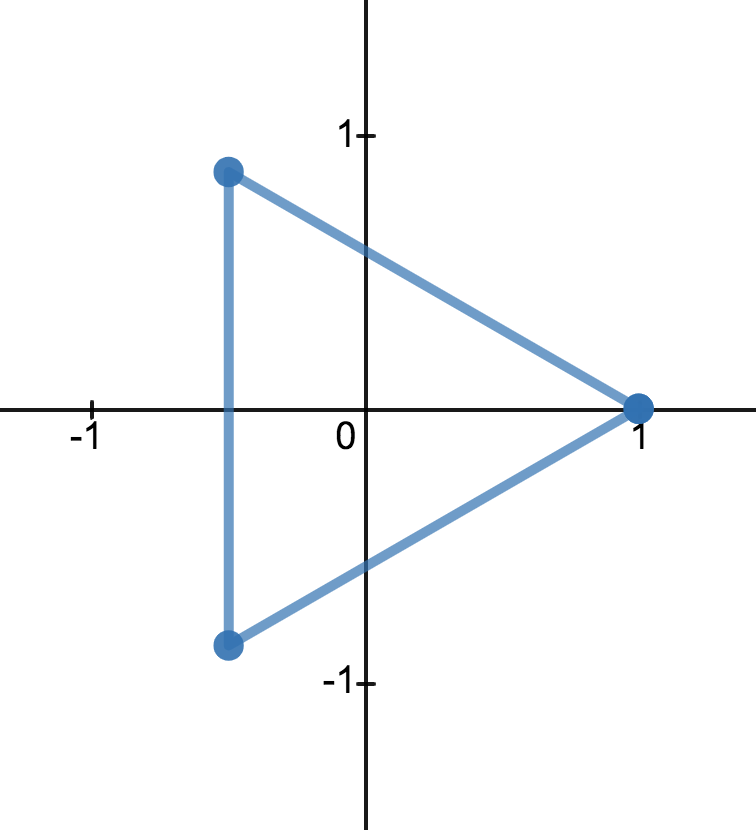
\includegraphics[width = 0.5\textwidth]{2.png}
            \caption{Take the triangle to have vertices at the cube roots of unity. Plotted in Desmos \cite{Desmos}.}
            \label{fig:Figure2}
        \end{figure}
        Clearly $\rho(e)$ is the $2 \times 2$ identity matrix. Now, instead of choosing $(1\,2)$ as our representative for the transpositions, pick $(2\,3)$ instead. Then 
        \begin{equation}
            \rho : (2\,3) \mapsto 
            \begin{bmatrix}
                1 & 0 \\
                0 & -1
            \end{bmatrix}.
        \end{equation}
        Lastly, $\rho \left( (1\,2\,3) \right)$ is rotation by $\frac{2\pi}{3}$ radians:
        \begin{equation}
            \rho : (1\,2\,3) \mapsto 
            \begin{bmatrix}
                \cos \left( \frac{2\pi }{3} \right) & -\sin \left( \frac{2\pi }{3} \right) \\[0.5em]
                \sin \left( \frac{2\pi }{3} \right) & \cos \left( \frac{2\pi }{3} \right)
            \end{bmatrix}
            =
            \begin{bmatrix}
                -\frac{1}{2} & -\frac{\sqrt{3}}{2} \\[0.5em]
                \frac{\sqrt{3}}{2} & -\frac{1}{2}
            \end{bmatrix}.
        \end{equation}
        We get the same two-dimensional representation since the characters line up.
    \end{enumerate}
    Finally, we have the full character table for $S_3$:
    \begin{table}[H]
        \centering
        \begin{tabular}{|| c || c | c | c ||}
            \hline
            class & $e$ & $(1\,2)$ & $(1\,2\,3)$ \\
            \hline
            $\chi_{\text{triv}}$ & $1$ & $1$ & $1$ \\
            $\chi_{\text{sign}}$ & $1$ & $-1$ & $1$ \\
            $\chi_3$ & $2$ & $0$ & $-1$ \\
            \hline
        \end{tabular}
        \caption{Full character table for $S_3$.}
        \label{tab:Table6}
    \end{table}
    Let's consider this character table as a matrix $U$. Orthogonality tells us that the rows are mutually orthogonal, if we weight the columns by the size of the classes: 
    \begin{equation}
        \begin{blockarray}{cccc}
              &  &  &  \\
            \begin{block}{c(ccc)}
            \frac{1}{6} \rightarrow & 1 & 1 & 1 \\[0.2 em]
            \frac{1}{6} \rightarrow & 1 & -1 & 1 \\[0.2 em]
            \frac{1}{6} \rightarrow & 2 & 0 & 1 \\
            \end{block}
        \end{blockarray}
        \begin{blockarray}{cccc}
              &  &  &  \\
            \begin{block}{c(ccc)}
            |[e]| = 1 \rightarrow & 1 & 1 & 2 \\[0.2 em]
            |[(1\,2)]| = 1 \rightarrow & 1 & -1 & 0 \\[0.2 em]
            |[(1\,2\,3)]| = 1 \rightarrow & 1 & 1 & -1 \\
            \end{block}
        \end{blockarray}
        =
        \begin{pmatrix}
            1 & 0 & 0 \\
            0 & 1 & 0 \\
            0 & 0 & 1
        \end{pmatrix}.
    \end{equation}
    Call the second matrix (unweighted) $\overline{U^t}$. Then 
    \begin{equation}
        \begin{split}
            \frac{1}{6} U 
            \begin{bmatrix}
                1 & 0 & 0 \\
                0 & 2 & 0 \\
                0 & 0 & 3
            \end{bmatrix}
            \overline{U^t} & = \Id \\
            \underbrace{U 
            \begin{bmatrix}
                1 & 0 & 0 \\
                0 & 2 & 0 \\
                0 & 0 & 3
            \end{bmatrix}}_{=:A}
            \underbrace{\overline{U^t}}_{=:B} & = 6 \Id.
        \end{split}
    \end{equation}
    Thankfully, if $AB = 6 \Id$, then $BA = 6 \Id$ (no silly stuff going on with left and right inverses not lining up, I'm looking at you, left and right shift operators!):
    \begin{equation}
        BA = \overline{U^t} U 
        \begin{bmatrix}
            1 & 0 & 0 \\
            0 & 2 & 0 \\
            0 & 0 & 3
        \end{bmatrix}
        = 6 \Id.
    \end{equation}
    %monky
    The rows of $\overline{U^t}$ are the columns of $U$, and the columns of 
    $U 
    \begin{bmatrix}
        1 & 0 & 0 \\
        0 & 2 & 0 \\
        0 & 0 & 3
    \end{bmatrix}$ are the weighted columns of $U$. So the columns are orthogonal too!
    
    So let $g , h \in G$ with conjugacy classes $[g]$, $[h]$ (maybe $g \simeq h$; maybe not). We just proved:
    \begin{equation}
        \left| [g] \right| \sum\limits_{i = 1}^r \chi_i(g) \overline{\chi_i(h)} = 
        \begin{cases}
            |G| , & \quad \text{if }g \sim h ,\\
            0 , & \quad \text{otherwise}
        \end{cases}.
    \end{equation}
    \begin{theorem}[Second Orthogonality]
        Let $g , h \in G$. Then 
        \begin{equation}
            \sum\limits_{i = 1}^r \chi_i(g) \overline{\chi_i(h)} = 
            \begin{cases}
                \frac{|G|}{\left| [g] \right|} , & \quad \text{if }g \sim h ,\\
                0 , & \quad \text{otherwise}
            \end{cases}.
        \end{equation}
    \end{theorem}
\end{enumerate}
\section{Handout: Basis Theorem}
\epigraph{``This skipping is another important point. It should be done whenever a proof seems too hard or whenever a theorem or a whole paragraph does not appeal to the reader.''}{Emil Artin}
\subsection{Dual Representations}
\begin{definition}
    Given a vector space $V$, the \textbf{dual vector space} is 
    \begin{equation}
        V^* \coloneqq  \Hom_k (V , k) = \setb{f : V \to k}.
    \end{equation}
\end{definition}
$V^*$ has an obvious structure as a vector space itself. It has the same dimension as $V$: Given a basis $\setb{e_1 , \dotsc, e_n}$ for $V$, the \textbf{dual basis} for $V^*$ is $\setb{f_1 , \dotsc, f_n}$, where $f_j(e_i) \coloneqq  \delta_{ij}$. 
\begin{remark}
    Strictly speaking, $V^*$ having the same dimension as $V$ only works when $V$ is finite-dimensional. When the dimension becomes infinite, things get much hairier. In the finite case, note that since $V$ and $V^*$ have the same dimension over the same field $k$, they are isomorphic, but not canonically so, as a basis for $V$ needs to be chosen.
\end{remark}
Given a representation $\rho : G \to \Aut(V)$, we can create the \textbf{dual representation} $\rho^* : G \to \Aut(V^*)$. We have three equivalent constructions:
\begin{enumerate}
    \item Given $g \in G$ and $f \in V^*$ (so $f : V \to k$), we need to define $\left[ \rho^*(g) \right](f) : V \to k$. Do this by composition:
    \begin{equation}
        \begin{tikzcd}
            V \arrow[r,"\rho(g)"] \arrow[d,"f"'] & V \arrow[dl] \\
            k
        \end{tikzcd}
    \end{equation}
    This makes $\left[ \rho^*g() \right](f) \circ \rho(g) = f$, so $\boxed{\left[ \rho^*(g) \right](f) = f \circ \inv{\rho(g)}.}$
    \item We have a \underline{bilinear form} $\vbrack{\cdot , \cdot} : V^* \times V \to k$ defined by $\vbrack{f , v} \coloneqq  f(v)$. Define $\rho^*(g)$ to satisfy $\vbrack{\rho^*(g)f , v} = \vbrack{f , \inv{\rho(g)} v}$.
    \begin{remark}
        This bilinear form is not quite the same as an inner product, though we can quickly make the connection: if $V$ has an inner product $\vbrack{\cdot , \cdot}_V : V \times V \to k$, then $V^*$ and $V$ \ita{are} canonically isomorphic via the correspondence $v \leftrightarrow f : w \mapsto \vbrack{v,w}_V$. 
    \end{remark}
\end{enumerate}
Either way, we get the equation $\left[ \rho^*(g) \right](f) = f \circ \inv{\rho(g)}$. The inverse seems awkward at first, but it is necessary to make $\rho^*$ a homomorphism:
\begin{equation}
    \begin{split}
        \rho^*(gh) & = f \circ \rho \left( \inv{(gh)} \right) \\
        & = f \circ \rho \left( \inv{h} \inv{g} \right) \\
        & = f \circ \rho \left( \inv{h} \right) \circ \rho \left( \inv{g} \right) \\
        & = \rho*(g) \left[ f \circ \rho \left( \inv{h} \right) \right] \\
        & = \rho*(g) \left[ \rho*(h) (f) \right] \\
        \rho^*(gh) & = \rho^*(g) \rho^*(h).
    \end{split}
\end{equation}
\begin{enumerate}[resume]
    \item Fix a basis $\setb{e_1 , \dotsc, e_n}$ for $V$ and the corresponding dual basis $\setb{f_1 , \dotsb, f_n}$ for $V^*$. In this basis, suppose $\rho \left( \inv{g} \right)$ is the matrix $A$; let's find the matrix for $\rho^*(g)$:
    \begin{equation}
        \left[ \rho^*(g) (f) \right](v) = \left[ f \circ \rho \left( \inv{g} \right) \right] (v) = f(Av).
    \end{equation}
    Now suppose $f = f_1$:
    \begin{equation}
        f : 
        \begin{bmatrix}
            1 \\
            0 \\
            \vdots \\
            0
        \end{bmatrix} 
        \mapsto 1,
        \begin{bmatrix}
            0 \\
            1 \\
            \vdots \\
            0
        \end{bmatrix}, \dotsc ,
        \begin{bmatrix}
            0 \\
            0 \\
            \vdots \\
            1
        \end{bmatrix} 
        \mapsto 0.
    \end{equation}
    Notice that $f$ acts as left multiplication by the row vector 
    $\begin{bmatrix}
        1 & 0 & \cdots & 0
    \end{bmatrix}$. 
    So calculating $f(Av)$ is the same as multiplying the first row of $A$ by $v$:
    \begin{equation}
        \begin{split}
            f(Av) & = 
            \begin{bmatrix}
                a_{11} & a_{12} & \cdots & a_{1n}
            \end{bmatrix} 
            \begin{bmatrix}
                v_1 \\
                v_2 \\
                \vdots \\
                v_n
            \end{bmatrix} \\
            & = a_{11} f_1(v) + a_{12} f_2(v) + \dotsb + a_{1n}f_n(v) \\
            \rho^*(g)(f) & = a_{11}f_1 + a_{12}f_2 + \dotsb + a_{1n}f_n.
        \end{split}
    \end{equation}
    So the first \underline{column} of the matrix for $\rho^*(g)$ is 
    $\begin{bmatrix}
        a_{11} \\
        a_{12} \\
        \vdots \\
        a_{1n}
    \end{bmatrix}$. Continuing, we can fill in each column:
    \begin{equation}
        \rho^*(g) = 
        \begin{bmatrix}
            a_{11} & a_{21} & \cdots & a_{n1} \\
            a_{12} & a_{22} & \cdots & a_{n2} \\
            \vdots & \vdots & \ddots & \vdots \\
            a_{1n} & a_{2n} & \cdots & a_{nn} 
        \end{bmatrix}
        = A^t = \boxed{ \left[ \inv{\rho(g)} \right]^t. }
    \end{equation}
    Again, this seems clumsy, but it works perfectly to make $\rho^*$ a homomorphism:
    \begin{equation}
        \begin{split}
            \rho^*(gh) & = \left[ \inv{\rho(gh)} \right]^t \\
            & = \left[ \inv{\rho(h)} \inv{\rho(g)} \right]^t \\
            & = \left[ \inv{\rho(g)} \right]^t \left[ \inv{\rho(h)} \right]^t \\
            & = \rho^*(g) \rho^*(h).
        \end{split}
    \end{equation}
\end{enumerate}
$\rho$ and $\rho^*$ always have the same dimension; sometimes they're isomorphic and sometimes not.
\subsection{Proof of the Basis Theorem}
\begin{theorem}[Dual Theorem]
    If $k \subseteq \cx$, then $\chi_{\rho^*} = \overline{\chi_{\rho}}$. 
\end{theorem}
\begin{proof}
    Working over $\cx$, we saw before that we can diagonalize our matrices, with roots of unity on the diagonal:
    \begin{equation}
        \rho(g) = 
        \begin{bmatrix}
            \omega_1 & 0 & \cdots & 0 \\
            0 & \omega_2 & \cdots & 0 \\
            \vdots & \vdots & \ddots & \vdots \\
            0 & 0 & \cdots & \omega_n \\
        \end{bmatrix}.
    \end{equation}
    Then 
    \begin{equation}
        \begin{split}
            \rho^*(g) & = \left[ \inv{\rho(g)} \right]^t \\
            & = \rho \left( \inv{g} \right)^t \\
            & = 
            \begin{bmatrix}
                \inv{\omega_1} & 0 & \cdots & 0 \\
                0 & \inv{\omega_2} & \cdots & 0 \\
                \vdots & \vdots & \ddots & \vdots \\
                0 & 0 & \cdots & \inv{\omega_n} \\
            \end{bmatrix}^t \\
            & = 
            \begin{bmatrix}
                \inv{\omega_1} & 0 & \cdots & 0 \\
                0 & \inv{\omega_2} & \cdots & 0 \\
                \vdots & \vdots & \ddots & \vdots \\
                0 & 0 & \cdots & \inv{\omega_n} \\
            \end{bmatrix}.
        \end{split}
    \end{equation}
    Therefore 
    \begin{equation}
        \begin{split}
            \chi_{\rho^*}(g) & = \inv{\omega_1} + \dotsb \inv{\omega_n} \\
            & = \overline{\omega_1} + \dotsb \overline{\omega_n} \qquad \text{since these are roots of unity} \\
            & = \overline{\omega_1 + \dotsb + \omega_n} \\
            & = \overline{\chi_{\rho}(g)}.
        \end{split}
    \end{equation}
\end{proof}
\begin{lemma}[Yet another Average Lemma]
    Let $\rho : G \to \Aut(V)$ be an irreducible representation of $G$ of dimension $n$ and $f : G \to \cx$ be a class function on $G$. (Recall that this means that $f \left( g h \inv{g} \right) = f(h)$.) Define 
    \begin{equation}
        \rho_f \coloneqq  \frac{1}{|G|} \sum\limits_{g \in G} f(g) \rho(g) \in \End_{\cx}(V).
    \end{equation}
    Then $\rho_f \in \End_{\cx G}(V)$ and $\rho_f = \frac{\vbrack{f , \chi_{\rho^*}}}{n} \Id$.
\end{lemma}
\begin{proof}[Proof of Yet another Average Lemma]
    $\rho_f$ is already a linear transformation; we need to show that it respects the $G$-action. So fix $h \in G$ and we will show that $\rho_f h = h \rho_f$. This is true if and only if $\inv{h} \rho_f h = \rho_f$. Let $v \in V$ and calculate: 
    \begin{equation}
        \inv{h} \rho_f h v = \frac{1}{|G|} \inv{h} \sum\limits_{g \in G} f(g) g h v.
    \end{equation}
    Let $r \coloneqq  \inv{h} g h$, so $g = h r \inv{h}$. As $g$ ranges over $G$, so does $r$:
    \begin{equation}
        \begin{split}
            \inv{h} \rho_f h v & = \frac{1}{|G|} \sum\limits_{g \in G} f(g) g h v \\
            & = \frac{1}{|G|} \inv{h} \sum\limits_{r \in G} f \left( h r \inv{h} \right) \left( h r \inv{h} \right) h v \\
            & = \frac{1}{|G|} \inv{h} \sum\limits_{r \in G} f(r) h r v \qquad \text{because $f$ is a class function} \\
            & = \frac{1}{|G|} \sum\limits_{r \in G} \inv{h} f(r) h r v \\
            & = \frac{1}{|G|} \sum\limits_{r \in G} f(r) \inv{h} h r v \qquad \text{because $f(r) \in \cx$ is a scalar} \\ 
            & = \frac{1}{|G|} \sum\limits_{r \in G} f(r) r v \\
            & = \rho_f v.
        \end{split}
    \end{equation}
    This proves that $\rho_f \in \End_{\cx G} (V)$, so by the Schur endomorphism corollary, (using $\rho$ irreducible) $\rho_f$ is a scalar operator: $\rho_f = \alpha \Id$ for some $\alpha \in \cx$. So let's calculate $\alpha$:
    \begin{equation}
        \begin{split}
            n \alpha & = \tr \rho_f \\
            & = \frac{1}{|G|} \sum\limits_{g \in G} f(g) \tr \rho(g) \\
            & = \frac{1}{|G|} \sum\limits_{g \in G} f(g) \chi_{\rho}(g) \\
            & = \frac{1}{|G|} \sum\limits_{g \in G} f(g) \overline{\chi_{\rho^*}(g)} \qquad \text{by the Dual Theorem} \\
            & = \left \langle f , \chi_{\rho^*} \right \rangle \\
            \alpha & = \boxed{ \frac{\left \langle f , \chi_{\rho^*} \right \rangle}{n} .}
        \end{split}
    \end{equation}
    This is what we needed to prove.
\end{proof}
\begin{proof}[Proof of the Basis Theorem]
    Let $\rho_1 , \dotsc , \rho_r$ be a complete set of irreducible representations with characters $\chi_1 , \dotsc , \chi_r$. We need to show that $\chi_i$'s span $\mathcal{F}_0[G]$. If not, then choose $f \in \mathcal{F}_0[G]$ that is orthogonal to all of the $\chi_i$'s. By Yet another Average Lemma, for any $i$, we have $\left( \rho_i \right)_f \in \End_{\cx G}(V)$ and $\left( \rho_i \right)_f = 0$ because $\left \langle f , \chi_{\rho_i} \right \rangle = 0$. Any other representation $\rho$ is built out of the $\rho_i$'s, so 
    \begin{equation}
        \begin{split}
            \rho_f & \coloneqq  \frac{1}{|G|} \sum\limits_{g \in G} f(g) \rho(g) \\
            & = \frac{1}{|G|} \sum\limits_{g \in G} \sum\limits_{i = 1}^r f(g) \rho_i(g) \\
            & = \sum\limits_{i = 1}^r \frac{1}{|G|} \sum\limits_{g \in G}f(g) \rho_i(g) \\
            & = \sum\limits_{i = 1}^r \left( \rho_i \right)_f = 0.
        \end{split}
    \end{equation}
    In particular, consider the regular representation $R$ with basis $\setb{g}_{g \in G}$. We have $R_f = 0$, meaning that 
    \begin{equation}
        \frac{1}{|G|} \sum\limits_{g \in G} f(g) R(g) = 0.
    \end{equation}
    Apply this to the vector $e \in V$, where $e$ is the identity element of the group $G$. We have $R(g)e = ge = g$ by definition of the regular representation, so 
    \begin{equation}
        \frac{1}{|G|} \sum\limits_{g \in G} f(g) g = 0
    \end{equation}
    as a vector in $V$. But the $g$ are linearly independent, so we must have every coefficient $f(g) = 0$. This shows that $f \equiv 0$, contradicting the choice of $f \in \mathcal{F}_0[G]$ as orthogonal to all of the $\chi_i$'s. So the $\chi_i$'s span $\mathcal{F}_0[G]$, and we are done.
\end{proof}
\section{March 16}
\subsection{Practice Blitz}
List all finite-dimensional division algebras over $\real$.
\section{March 18}
\subsection{Fake Blitz}
I have a representation $\rho : S_3 \to \Aut(\cx^{12})$ as follows: [get source code from Dr. Murray]

Decompose $\rho$ into irreducibles.
\subsection{Example: Character Table for \texorpdfstring{$A_4$}{A4}}
A set of class representatives in $S_4$ are 
\begin{equation}
    [e] = \setb{e} \,,\,  [(1\,2)] \,,\, [(1\,2\,3)] \,,\, [(1\,2)(3\,4)] \,,\, [(1\,2\,3\,4)].
\end{equation}
The even ones are $[e]$, $[(1\,2\,3)]$, and $[(1\,2)(3\,4)]$, but the class of $(1\,2\,3)$ has 8 elements. As the orders of the conjugacy classes must divide the order of the group (Orbit-Stabilizer Formula!), the class of $(1\,2\,3)$ splits into the class of $(1\,2\,3)$ and $(1\,3\,2)$ in $A_4$. 

To find one-dimensional representations, let's abelianize $A_4$:
\begin{equation}
    [A_4 , A_4] = \vbrack{(1\,2)(3\,4) , (1\,3)(2\,4)} \simeq K_4,
\end{equation}
so 
\begin{equation}
    A_4^{ab} = \quotient{A_4}{A_4 , A_4]} = \left \langle \overline{(1\,2\,3)} \right \rangle \simeq \z_3.
\end{equation}
This gives us 3 one-dimensional representations: let 
\begin{equation}
    \omega \coloneqq  e^{\frac{2\pi i}{3}}.
\end{equation}
Then each of the one dimensional representations is determined by $(1\,2\,3) \mapsto \omega^j$ for $j \in \setb{0,1,2}$. Note that since the class of $(1\,2)(3\,4)$ is in $[A_4 , A_4]$, these all get sent to $1$.

There are four conjugacy classes in $A_4$, and 
\begin{equation}
    12 = 1^2 + 1^2 + 1^2 + 3^2,
\end{equation}
so we have one 3-dimensional representation. We could determine this from orthogonality, but it's more fun to find it geometrically:

Recall that $A_4$ is the symmetry group of the \underline{tetrahedron}, acting by permutations on the corners. This gives us an action of $A_4$ on $\real^3$. Finding all these matrices using a single basis would be nasty, but we don't have to, because we only want their traces. So we can use whatever basis we want for each matrix.
\begin{figure}[H]
    \centering
    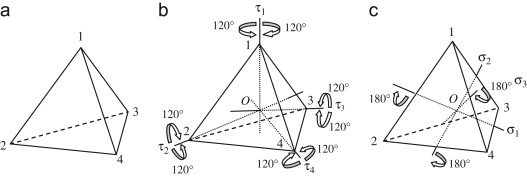
\includegraphics[width = 0.5\textwidth]{3.jpg}
    \caption{The symmetry group of a tetrahedron has order 12. It turns out this group is exactly $A_4$. From \url{https://www.sciencedirect.com/science/article/pii/S002250961200110X}.}
    \label{fig:Figure3}
\end{figure}
Now, every rotation $R$ in $\real^3$ has an eigenvalue. This is because its characteristic polynomial is a cubic, and every cubic has at least \underline{real} one root (Intermediate Value Theorem!). Hence every rotation has a one-dimensional invariant subspace, and it is exactly axis of that rotation. Thus $R$ is just rotation by some angle $\theta$ about that axis, and so in an appropriate basis, every rotation can be written as 
\begin{equation}
    \left[
        \begin{array}{c | c c}
            1 & 0 & 0 \\
            \hline 
            0 & \cos \theta & -\sin \theta \\
            0 & \sin \theta & \cos \theta
        \end{array}
    \right].
\end{equation}
The trace is then $1 + 2\cos \theta$, so we only need to know $\theta$. Now, $(1\,2)(3\,4)$ has order 2, so it must be a rotation by $\pi$. Thus 
\begin{equation}
    \chi : (1\,2)(3\,4) \mapsto 1 + 2 \cos \pi = -1.
\end{equation}
$(1\,2\,3)$ has order 3; it rotates the tetrahedron around one vertex. This gives us $\chi \left( (1\,2\,3) \right) = \chi \left( (1\,3\,2) \right) = 0$, and so we have fully determined the three-dimensional representation.
\begin{table}[H]
    \centering
    \begin{tabular}{|| c || c | c | c | c ||}
        \hline
        class & $e$ & $(1\,2)(3\,4)$ & $(1\,2\,3)$ & $(1\,3\,2)$ \\
        \hline
        size of class & $1$ & $3$ & $4$ & $4$ \\
        \hline 
        $\chi_{\text{triv}}$ & $1$ & $1$ & $1$ & $1$ \\
        $\chi_{\omega}$ & $1$ & $1$ & $\omega$ & $\omega^2$ \\
        $\chi_{\omega^2}$ & $1$ & $1$ & $\omega^2$ & $\omega$ \\
        $\chi_{3}$ & $3$ & $-1$ & $0$ & $0$ \\
        \hline
    \end{tabular}
    \caption{Character table for $A_4$. Note that for $A_4$, $\rho_{\text{triv}} = \rho_{\text{sign}}$.}
    \label{tab:Table7}
\end{table}
\subsection{Quick Aside on Computing Inner Products}
\begin{remark}
    This is all original material from me, with some input from Rami Allaf.
\end{remark}
Recall that our definition of inner product on $\mathcal{F}[G]$: 
\begin{equation}
    \vbrack{\phi , \psi} \coloneqq  \frac{1}{|G|} \sum\limits_{g \in G} \phi(g) \overline{\psi(g)}.
\end{equation}
We can treat this inner product literally as the dot product between complex vectors, with a normalization factor: if we order the elements of $G$ as $\setb{g_1 = e , g_2 , \dotsc , g_n}$ (where $n\coloneqq |G|$), then we can write elements of $\mathcal{F}[G]$ as vectors in $\cx^n$, by 
\begin{equation}
    \phi \xlongleftrightarrow{} 
    \begin{bmatrix}
        \phi(e) \\
        \phi(g_2) \\
        \ddots \\
        \phi(g_n)
    \end{bmatrix}.
\end{equation}
Then the inner product becomes 
\begin{equation}
    \vbrack{\phi , \psi} \coloneqq  \frac{1}{n} \phi^t \overline{\psi},
\end{equation}
Now, when we're computing inner products of characters, we don't to compute $n$ products since characters are class functions. So instead of treating $\chi \in \cx^n$, we can instead treat $\chi \in \cx^r$, where $r$ is the number of conjugacy classes of $G$. Choose an ordered set $\setb{g_1 = e , g_2 , \dotsc , g_r}$ of representatives for each conjugacy class, then 
\begin{equation}
    \chi \xlongleftrightarrow{} 
    \begin{bmatrix}
        \chi(e) \\
        \chi(g_2) \\
        \ddots \\
        \chi(g_r)
    \end{bmatrix}.
\end{equation}
Now, to compute the inner product, we form a matrix $W \in \m_n(\cx)$ of ``weights'' with the sizes of the conjugacy classes along its diagonal (according to the specified order), and zero elsewhere.
\begin{equation}
    W = 
    \begin{bmatrix}
        1 & 0 & \cdots & 0 \\
        0 & |[g_2]| & \cdots & 0 \\
        \vdots & \vdots & \ddots & \vdots \\
        0 & 0 & \cdots & |[g_r]|
    \end{bmatrix}.
\end{equation}
Note that $W$ is actually invertible, and that $\tr(W) = n = |G|$. Then the inner product between two characters $\chi_1$ and $\chi_2$ is given by 
\begin{equation}
    \vbrack{\chi_1 , \chi_2} = \frac{1}{n} \chi_1^t W \overline{\chi_2}.
\end{equation}
This approach is really only helpful for nonabelian groups, and in particular those with trivial centers (like $S_n$). In the case where $G$ is abelian, every element is its own conjugacy class and so we're back to square one.

Now, for the sake of forming some analogies with Quantum Mechanics, let's switch things up a bit. Let's redefine the inner product without the normalization and with complex conjugation on the first term:
\begin{equation}
    \vbrack{\chi_1 , \chi_2}_{\text{new}} \coloneqq  \chi_1^{\ast} \chi_2,
\end{equation}
where the asterisk denotes conjugate transpose. Let's take the Quantum analogy even further and adopt the physics notation, with bras and kets:
\begin{equation}
    \vbrack{\chi_1 \mid \chi_2} \coloneqq  \chi_1^{\dagger} \chi_2,
\end{equation}
Now, redefine the weight matrix $W$ to have the normalization factor of $\frac{1}{n}$:
\begin{equation}
    \tilde{W} \coloneqq  \frac{1}{n} W.
\end{equation}
Note that $\tr \left( \tilde{W} \right) = 1$. Then the inner product of two characters becomes
\begin{equation}
    \vbrack{\chi_1 , \chi_2}_{\text{original}} = \langle \chi_1 \mid \tilde{W} \mid \chi_2 \rangle.
\end{equation}
Now, if we take the inner product of a character with itself, we can interpret that as a sort of ``expectation value'' of $\tilde{W}$ in the ``state $\mid \chi \rangle$.''
\section{March 23: Restriction and Induction}
Let $G$ be a group with subgroup $H$ (not necessarily normal or even nontrivial; yes, even $H \coloneqq  \setb{e}$ is interesting). Restriction takes us from a representation of $G$ to one of $H$, and Induction goes the opposite way:
\begin{equation}
    \begin{tikzcd}
        G \arrow[d,xshift=-0.7ex,"\text{Res}"'] \\
        H \arrow[u,xshift=0.7ex, "\text{Ind}"']
    \end{tikzcd}
\end{equation}
Restriction is much simpler, but they play complementary roles (in a way made precise by \underline{Frobenius Reciprocity}), so we study them together.
\subsection{Restriction}
Given a representation $\rho : G \to \Aut(V)$, we can \underline{restrict} it to $H$:
\begin{equation}
    \begin{split}
        \rho \big\downarrow_H^G & : H \to \Aut(V) \\
        \rho \big\downarrow_H^G(h) & \coloneqq  \rho(h).
    \end{split}
\end{equation}
Now we have a representation of $H$. You just use the same matrix for $h \in H$ that you would by considering $h \in G$. That was easy, wasn't it?
\begin{remark}
    Warning! Elements of $H$ that were conjugate in $G$ might no longer be conjugate in $H$. For example, $(1\,2\,3)$ and $(1\,3\,2)$ are conjugate in $G \coloneqq  S_4$, but not in $H \coloneqq  A_4$.
\end{remark}
\subsection{Tensor Products of Modules}
Induction is trickier than restriction. First we need a crash course in tensor products.
\begin{definition}
    Let $R$ be a ring. Start with a right $R$-module $M_R$ and a left $R$-module $_RN$. We can form their \textbf{tensor product} $M \otimes_R N$: 
    \begin{equation}
        M \otimes_R N \coloneqq  \left \{ \sum\limits_{i = 1}^n m_i \otimes n_i \, \middle| \, n \in \z^+ , m_i \in M , n_i \in N\right \} \bigg/ \sim,
    \end{equation}
    where $\sim$ is the set of relations to define \textbf{bilinearity}:
    \begin{equation}
        \begin{split}
            m \otimes (n_1 + n_2) & = m \otimes n_1 + m \otimes n_2 \\
            (m_1 + m_2) \otimes n & = m_1 \otimes n + m_2 \otimes n \\
            m r \otimes n & = m \otimes rn.
        \end{split}
    \end{equation}
\end{definition}
Note that $M \otimes_R N$ by itself is \ita{not} an $R$-module; there is no consistent way for $R$ to act on either side of it. Instead, $M \otimes_R N$ is just an abelian group, that is, a $\z$-module. 

Now, suppose that $M$ is actually an \underline{$S$-$R$-bimodule}, that is, a left module over a ring $S$ and right module over $R$ such that the actions commute: $(sm)r = s(mr)$ for all $s \in S$, $r \in R$, $m \in M$. This would make $M \otimes_R N$ into a left $S$-module via $s ( m \otimes n ) = (sm) \otimes n$.

A common application of this is \underline{scalar extension}, when we've built some construction over one ring $R$ and we want to build a similar construction over a larger ring $S \supseteq R$.

For example, let $k \subseteq K$ be fields. (Think of your favorite vector space over $\q$. How can we make it into a vector space over $\real$?)

If we have a vector space $_kW$, we can extend to a vector space $_K \overline{W}$ by taking $\overline{W} \coloneqq  K \otimes_k W$. This is a left $K$-module (that is, a $K$-vector space) via the left multiplication of $K$ on itself. Given a $k$-basis $\setb{w_1 , \dotsc , w_n}$ for $W$, we have a $K$-basis $\setb{ 1 \otimes w_1 , \dotsc , 1 \otimes w_n }$ for $\overline{W}$.
\begin{example}
    Take $k \coloneqq  \q$ and $_kW$ to be the \underline{rational} quaternions:
    \begin{equation}
        _{\q} W \coloneqq  \setb{ a + bi + cj + dk \mid a , b , c , d \in \q }.
    \end{equation}
    Then $\overline{W} = \real \otimes_{\q} W$ is the span of $1 \otimes 1$, $1 \otimes i$, $1 \otimes j$, and $1 \otimes k$ over $\real$, which is the real quaternions $\h$.
\end{example}
\subsection{Induced Representations}
 \begin{remark}
    No, this is not mathematical induction, nor is it Faraday's law of induction!
    \begin{align}
        P_n & \implies P_{n+1} \\
        \nabla \times \mathbf{E} & = -\frac{\partial \mathbf{B}}{\partial t}.
    \end{align}
    Not those! Induction is one of those overused words in mathematics.
\end{remark}
Start with a group $G$ with a subgroup $H \leq G$, and a representation $\rho : H \to \Aut(W)$. Then we can identify $W$ as a left $kH$-module. Note that $kH \subseteq kG$ as $k$-algebras. So consider $kG$ as a right $kH$-module and form the tensor product $V \coloneqq  kG \otimes_{kH} W$. Now, again as above, consider $_{kG} kG$ as a left module over itself. So, still as above, the tensor product $V \coloneqq  kG \otimes_{kH} W$ is a left $kG$-module. But that is the same as a representation!
\begin{equation}
    \begin{split}
        \rho \big\uparrow_H^G & : G \to \Aut(V) = \Aut(kG \otimes_{kH} W) \\
        g ( r \otimes w) & \coloneqq  (gr) \otimes w.
    \end{split}
\end{equation}
That was the definition, but it is not obvious what $_{kG}V$ looks like, so let's break it down: 

First off, let $\setb{w_1 , \dotsc , w_n}$ be a basis for $W$ over $k$. We know that $\setb{ g }_{g \in G}$ is a basis for $kG$ over $k$. So the vectors $\setb{g \otimes w_i \mid g \in G , i = 1 , \dotsc , n}$ span $V$ over $k$.

However, these vectors are not all linearly independent, because we are tensoring over $kH$, not over $k$. This introduces some extra relations: 

Suppose, in $G$, that $g_1 \equiv g_2$ (mod $H$), that is, that $g_1 H = g_2 H$, that is $\overline{g_1} = \overline{g_2}$ in $\quotient{G}{H}$. (Remember that we aren't requiring $H \trianglelefteq G$, so $\quotient{G}{H}$ isn't necessarily a group, just a set of cosets.)

By the old coset criterion, we have $g_1 = g_2 h$ for some $h \in H$ ; then 
\begin{equation}
    g_1 \otimes w_i = g_2 h \otimes w_i = g_2 \otimes h w_i \in g_2 \otimes W.
\end{equation}
So $g_1 \otimes W = g_2 \otimes W$. So we need not consider all $g \in G$, just a set of coset representatives $t_1 , \dotsc , t_r$ for $\quotient{G}{H}$, where $r \coloneqq  [G : H]$. Fix such a set of representatives; then 
\begin{equation}
    V = kG \otimes_{kH} W = t_1 \otimes W \oplus \dotsb \oplus t_r \otimes W.
\end{equation}
Taking dimensions of both sides gives 
\begin{equation}
    \dim_k V = r \dim_k W = \boxed{[G : H] \dim_k W.}
\end{equation}
So $V$ is built out of $r = [G : H]$ chunks of the form $t_i \otimes W$.

Now let's use the matrices for $\rho$ to find matrices for $\rho \big\uparrow_H^G$. Consider the $t_i \otimes W$'s as blocks and write a block matrix: 
\begin{equation}
    \rho \big\uparrow_H^G(g) = 
    \left[\def\arraystretch{1.5}
    \begin{array}{c | c | c | c}
        \varrho_{11} & \varrho_{12} & \cdots & \varrho_{1r} \\
        \hline
        \varrho_{21} & \varrho_{22} & \cdots & \varrho_{2r} \\
        \hline 
        \vdots & \vdots & \ddots & \vdots \\
        \hline
        \varrho_{r1} & \varrho_{r2} & \cdots & \varrho_{rr}
    \end{array}
    \right]
    \left[\def\arraystretch{1.5}
    \begin{array}{c}
        t_1 \otimes W \\
        \hline
        t_2 \otimes W \\
        \hline 
        \vdots \\
        \hline
        t_r \otimes W
    \end{array}
    \right]
    \xlongrightarrow{}
    \left[\def\arraystretch{1.5}
    \begin{array}{c}
        t_1 \otimes W \\
        \hline
        t_2 \otimes W \\
        \hline 
        \vdots \\
        \hline
        t_r \otimes W
    \end{array}
    \right],
\end{equation}
where $\varrho_{ij}$ is the matrix taking $t_j \otimes W$ to $t_i \otimes W$. Let's calculate this block: 
\begin{equation}
    g ( t_j \otimes W ) \coloneqq  (g t_j) \otimes W \stackrel{?}{\subseteq} t_i \otimes W.
\end{equation}
By our coset criterion, this can happen if and only if $g t_j \equiv t_i$ (mod $H$), if and only if $\inv{t_i} g t_j \in H$. So the matrix in this block is $\rho \left( \inv{t_i} g t_j \right)$ if $\inv{t_i} g t_j \in H$ and $0$ otherwise. Applying this idea, we get the matrix for $\rho \big\uparrow_H^G(g)$:
\begin{equation}
    \boxed{
        \rho \big\uparrow_H^G(g) = 
        \left[\def\arraystretch{1.5}
        \begin{array}{c | c | c | c}
            \rho \left( \inv{t_1} g t_1 \right) & \rho \left( \inv{t_1} g t_2 \right) & \cdots & \rho \left( \inv{t_1} g t_r \right) \\
            \hline
            \rho \left( \inv{t_2} g t_1 \right) & \rho \left( \inv{t_2} g t_2 \right) & \cdots & \rho \left( \inv{t_2} g t_r \right) \\
            \hline 
            \vdots & \vdots & \ddots & \vdots \\
            \hline
            \rho \left( \inv{t_r} g t_1 \right) & \rho \left( \inv{t_r} g t_2 \right) & \cdots & \rho \left( \inv{t_r} g t_r \right)
        \end{array}
        \right]
    },
\end{equation}
where $\rho \left( \inv{t_i} g t_j \right)$ is the old matrix for $\rho$ if $\inv{t_i} g t_j \in H$ and we define $\rho \left( \inv{t_i} g t_j \right) = 0$ if $\inv{t_i} g t_j \notin H$.
\subsection{Group Blitz}
Complete the character table for $S_4$:
\begin{table}[H]
    \centering
    \begin{tabular}{|| c || c | c | c | c | c ||}
        \hline
        class & $e$ & $(1\,2)$ & $(1\,2\,3)$ & $(1\,2\,3\,4)$ & $(1\,2)(3\,4)$ \\
        \hline
        size of class & $1$ &  &  &  &  \\
        \hline
        $\chi_{\text{triv}}$ & & & & & \\
        $\chi_{\text{sign}}$ & & & & & \\
        $\chi_{\text{cube}}$ & $3$ & $1 + 2 \cos \left( \theta_{(12)}\right)$ & $1 + 2 \cos \left( \theta_{(123)}\right)$ & $1 + 2 \cos \left( \theta_{(1234)}\right)$ & $1 + 2 \cos \left( \theta_{(12)(34)}\right)$ \\
        $\chi_{\text{sign} \otimes \text{cube}}$ & & & & & \\
        $\chi_{\text{mystery}}$ & & & & & \\
        \hline
    \end{tabular}
    \caption{}
    \label{tab:Table8}
\end{table}
\section{March 25}
\subsection{Blitz}
Given $H \leq G$, $\rho : H \to \Aut(W)$, what is the strongest structure you can put on $kG \otimes_{kH} W$?
\subsection{Examples of Induced Representations}
\begin{example} 
    \noindent
    \begin{enumerate}
        \item Let's work in the dihedral group: 
        \begin{equation}
            \begin{split}
                G & \coloneqq  D_n = \vbrack{ r , s \mid r^4 = s^2 = e , srs = \inv{r}} \\
                H & \coloneqq  \vbrack{r} = \setb{e , r , r^2 , \dotsc , r^{n-1}} \simeq \z_n.
            \end{split}
        \end{equation}
        Since $\z_n$ is abelian, the irreducible complex representations are one-dimensional, so they are homomorphisms $\rho : \z_n \to \cx^{\times}$. There are $n$ such homomorphisms given by $\rho_j : r \mapsto \omega^j$, where 
        \begin{equation}
            \omega \coloneqq  e^{\frac{2\pi i}{n}}.
        \end{equation}
        Let's calculate $\rho_j \big\uparrow_H^G$: first, we choose a set of coset representatives for $\quotient{G}{H}$. We'll use $t_1 \coloneqq  eH$, $t_2 \coloneqq  sH$. Now let's find $\rho_j \big\uparrow_H^G(g)$ for the generators $g \coloneqq  r$ and $g \coloneqq  s$.
        \begin{equation}
            \begin{split}
                \rho_j \big\uparrow_H^G(r) & = 
                \left[\def\arraystretch{1.2}
                \begin{array}{c | c}
                    \rho \left( \inv{t_1} r t_1 \right) & \rho \left( \inv{t_1} r t_2 \right) \\
                    \hline
                    \rho \left( \inv{t_2} r t_1 \right) & \rho \left( \inv{t_2} r t_2 \right)
                \end{array}
                \right] \\
                & = 
                \left[\def\arraystretch{1.2}
                \begin{array}{c | c}
                    \rho (r) & \rho (rs) \\
                    \hline
                    \rho (sr) & \rho (srs) = \rho \left( \inv{r} \right)
                \end{array}
                \right] \\
                & = 
                \left[\def\arraystretch{1.2}
                \begin{array}{c | c}
                    \omega^j & 0 \\
                    \hline
                    0 & \omega^{-j}
                \end{array}
                \right], \\
                \rho_j \big\uparrow_H^G(s) & = 
                \left[\def\arraystretch{1.2}
                \begin{array}{c | c}
                    \rho \left( \inv{t_1} s t_1 \right) & \rho \left( \inv{t_1} s t_2 \right) \\
                    \hline
                    \rho \left( \inv{t_2} s t_1 \right) & \rho \left( \inv{t_2} s t_2 \right)
                \end{array}
                \right] \\
                & = 
                \left[\def\arraystretch{1.2}
                \begin{array}{c | c}
                    \rho (s) & \rho (e) \\
                    \hline
                    \rho (e) & \rho (s) 
                \end{array}
                \right] \\
                & = 
                \left[\def\arraystretch{1.2}
                \begin{array}{c | c}
                    0 & 1 \\
                    \hline
                    1 & 0
                \end{array}
                \right].
            \end{split}
        \end{equation}
        So now we have a 2-dimensional representation of $D_n$. Have we seen it before? Let's compute its characters:
        \begin{equation}
            \begin{split}
                \chi_{\rho_j \uparrow}(r) & = \omega^j + \omega^{-j} \\
                & = \cos \left( \frac{2 \pi j}{n} \right) + i \sin \left( \frac{2 \pi j}{n} \right) + \cos \left( \frac{2 \pi j}{n} \right) - i \sin \left( \frac{2 \pi j}{n} \right) \\
                & = 2 \cos \left( \frac{2 \pi j}{n} \right),\\
                \chi_{\rho_j \uparrow}(s) & = 0.
            \end{split}
        \end{equation}
        This agrees with the character of the 2-dimensional $\rho$-tation representation that we found before by letting $D_n$ act on $\real^2$ (or $\cx^2$) by rotating the plane through an angle of $\theta_j \coloneqq  \frac{2 \pi j}{n}$:
        \begin{equation}
            \rho_j : r \mapsto 
            \begin{bmatrix}
                \cos \theta_j & -\sin \theta_j \\
                \sin \theta_j & \cos \theta_j
            \end{bmatrix}, \qquad \rho_j : s \mapsto
            \begin{bmatrix}
                -1 & 0 \\
                0 & 1
            \end{bmatrix}.
        \end{equation}
        Since the characters agree, they must be the same representation, just in a different basis.
        \item Let $G$ be any finite group, and let $H \coloneqq  \setb{e}$. $H$ has only the trivial representation $\rho(e) \coloneqq  1$. Let's find $\rho_j \big\uparrow_H^G$. A set of coset representatives for $\quotient{G}{H}$ is just the whole group $G$, let's still label them $t_1 , \dotsc, t_n$. 
        
        The $ij$ entry of $\rho_j \big\uparrow_H^G(g)$ is $0$ if $\inv{t_i} g t_j \notin H$, and $1$ if $\inv{t_i} g t_j \in H$, that is, if $\inv{t_i} g t_j = e$, if and only if $g t_i = t_j$. We have exactly the regular representation of $G$.
    \end{enumerate}
\end{example}
\begin{theorem}[Induced Character Theorem]
    \noindent
    \begin{enumerate}
        \item Let $\setb{t_1 , \dotsc , t_r}$ be a set of coset representatives for $\quotient{G}{H}$. Then for $g \in $G, we have
        \begin{equation}
            \chi_{\rho \uparrow}(g) = \sum\limits_{i = 1}^r \chi_{\rho} \left( \inv{t_i} g t_i \right),
        \end{equation}
        where we understand $\chi_{\rho} \left( \inv{t_i} g t_i \right)$ to mean $0$ if $\inv{t_i} g t_i \notin H$.
        \item If $g \notin \bigcup\limits_{t \in G} \inv{t} H t$, then $\chi_{\rho \uparrow}(g) = 0$.
    \end{enumerate}
\end{theorem}
\subsection{Frobenius Reciprocity}
Suppose you have a subgroup $H \leq G$ (not necessarily normal) and one representation at each level:
\begin{equation}
    \begin{split}
        \sigma & : G \to \Aut(V) \\
        \rho & : H \to \Aut(W).
    \end{split}
\end{equation}
Let's draw a diagram!
\begin{equation}
    \begin{tikzcd}
        G \arrow[d,xshift=-0.7ex,bend right=60,"\sigma \downarrow"'] \\
        H \arrow[u,xshift=0.7ex,bend right=60,"\rho \uparrow"']
    \end{tikzcd}
\end{equation}
The celebrated formula for \textbf{Frobenius Reciprocity} describes what happens when the representations meet at the different levels, that is, what happens when $\rho$ meets $\sigma$ at the $G$ level, versus when $\rho$ meets $\sigma$ at the $H$ level. The computation formulation is given by:
\begin{equation}
    \boxed{ \vbrack{ \chi_{\rho \uparrow} , \chi_{\sigma} }_G = \vbrack{ \chi_{\rho} , \chi_{\sigma \downarrow}}_H. }
\end{equation}
Here the subscripts mean that the inner product on the LHS is taken over $G$ and the one on the RHS is taken over $H$.
\begin{proof}
    \begin{equation}
        \begin{split}
            \vbrack{ \chi_{\rho \uparrow} , \chi_{\sigma} }_G & = \frac{1}{|G|} \sum\limits_{g \in G} \chi_{\rho \uparrow}(g) \overline{ \chi_{\sigma}(g) } \\
            & = \frac{1}{|G|} \sum\limits_{g \in G} \sum\limits_{i = 1}^r \chi_{\rho} \left( \inv{t_i} g t_i \right) \overline{ \chi_{\sigma}(g) } \\
            & = \frac{1}{|G|} \sum\limits_{i = 1}^r \sum\limits_{g \in G} \chi_{\rho} \left( \inv{t_i} g t_i \right) \overline{ \chi_{\sigma}(g) }.
        \end{split}
    \end{equation}
    So $\left( \inv{t_i} g t_i \right)$ doesn't (necessarily) vanish if $\inv{t_i} g t_i \in H$. As $g$ ranges over $G$, $\inv{t_i} g t_i$ also ranges over all of $G$, but it only matters when $\inv{t_i} g t_i = h \in H$ (so $g = t_i h \inv{t_i}$). So 
    \begin{equation}
        \begin{split}
            \vbrack{ \chi_{\rho \uparrow} , \chi_{\sigma} }_G & = \frac{1}{|G|} \sum\limits_{i = 1}^r \sum\limits_{g \in G} \chi_{\rho}(h) \overline{\chi_{\sigma} \left( t_i h \inv{t_i} \right) } \\
            & = \frac{1}{|G|} \sum\limits_{i = 1}^r \sum\limits_{g \in G} \chi_{\rho}(h) \overline{\chi_{\sigma} (h) } \\
            & = \frac{r}{|G|} \sum\limits_{h \in H} \chi_{\rho}(h) \overline{\chi_{\sigma} (h) }.
        \end{split}
    \end{equation}
    Since $r = [G : H] = \frac{|G|}{|H|}$, 
    \begin{equation}
        \begin{split}
            \vbrack{ \chi_{\rho \uparrow} , \chi_{\sigma} }_G & = \frac{1}{|G|} \frac{|G|}{|H|} \sum\limits_{h \in H} \chi_{\rho}(h) \overline{\chi_{\sigma} (h) } \\
            & = \frac{1}{|H|} \sum\limits_{h \in H} \chi_{\rho}(h) \overline{\chi_{\sigma} (h) } \\
            & = \vbrack{ \chi_{\rho} , \chi_{\sigma \downarrow}}_H.
        \end{split}
    \end{equation}
\end{proof}

\section{April 6}
\subsection{Blitz}
Let $H \coloneqq  A_4$, $G \coloneqq  S_4$, $\rho : H \to \Aut(\cx^5)$. What is $\chi_{\rho \uparrow_H^G}(e)$?
\subsection{Frobenius Reciprocity (cont'd)}
\begin{example}
    \noindent
    \begin{itemize}
        \item Let $\rho$ be the Permutation representation on $H \coloneqq  S_3$, and let $\sigma$ be the tensor product of the sign and cube representations of $G \coloneqq  S_4$. (We also saw this as $U$). Let's calculate both sides:
        \begin{table}[H]
            \centering
            \begin{tabular}{|| c | c | c | c ||}
                \hline
                class & $e$ & $(1\,2)$ & $(1\,2\,3)$ \\
                size of class & $1$ & $3$ & $2$ \\
                \hline
                $\chi_{\rho}$ & $3$ & $1$ & $0$ \\
                $\chi_{\sigma \downarrow}$ & $3$ & $1$ & $0$ \\
                \hline
            \end{tabular}
            \caption{}
            \label{tab:Table9}
        \end{table}
        Thus 
        \begin{equation}
            \begin{split}
                \vbrack{ \chi_{\rho} , \chi_{\sigma \downarrow} }_H & = \frac{1 \cdot 3^2 + 3 \cdot 1^2 + 2 \cdot 0^2}{6} \\
                & = \frac{9 + 3}{6} \\
                & = \boxed{2.}
            \end{split}
        \end{equation}
        To find $\chi_{\rho \uparrow}$, use the Induced character theorem with coset representatives
        \begin{equation}
            \quotient{S_4}{S_3} = \setb{t_1 \coloneqq  e , t_2 \coloneqq  (1\,4) , t_3 \coloneqq  (2\,4) , t_4 \coloneqq  (3\,4)}
        \end{equation}
        Then 
        \begin{equation}
            \begin{split}
                \chi_{\rho \uparrow}(e) & = [S_4 : S_3] \chi_{\rho}(e) = 4 \times 3 = \boxed{12.} \\
                \chi_{\rho \uparrow} \left( (1\,2) \right) & = \cancelto{1}{\chi_{\rho} \left( (1\,2) \right)} + \cancelto{0}{\chi_{\rho} \left( (1\,4)(1\,2)(1\,4) \right)} \\
                & + \cancelto{0}{\chi_{\rho} \left( (2\,4)(1\,2)(2\,4) \right)} + \cancelto{1}{\chi_{\rho} \left( (3\,4)(1\,2)(3\,4) \right)} \\
                & = \boxed{2.} \\
                \chi_{\rho \uparrow} \left( (1\,2\,3) \right) & = \cancelto{0}{\chi_{\rho} \left( (1\,2\,3) \right)} + \cancelto{0}{\chi_{\rho} \left( (1\,4)(1\,2\,3)(1\,4) \right)} \\
                & + \cancelto{0}{\chi_{\rho} \left( (2\,4)(1\,2\,3)(2\,4) \right)} + \cancelto{0}{\chi_{\rho} \left( (3\,4)(1\,2\,3)(3\,4) \right)} \\
                & = \boxed{0.} \\
                \chi_{\rho \uparrow} \left( (1\,2\,3\,4) \right) & = \sum\limits_{i = 1}^4 \chi_{\rho} \left( \text{a 4-cycle} \right) = \boxed{0.} \\
                \chi_{\rho \uparrow} \left( (1\,2)(3\,4) \right) & = \sum\limits_{i = 1}^4 \chi_{\rho} \left( (a\,b)(c\,d) \right) = \boxed{0.}
            \end{split}
        \end{equation}
        Then 
        \begin{equation}
            \begin{split}
                \vbrack{\chi_{\rho \uparrow} , \chi_{\sigma}}_G & = \frac{36 + 12}{24} \\
                & = \frac{48}{12} \\
                & = \boxed{2.}
            \end{split}
        \end{equation}
        \begin{table}[H]
            \centering
            \begin{tabular}{|| c | c | c | c | c | c ||}
                \hline
                class & $e$ & $(1\,2)$ & $(1\,2\,3)$ & $(1\,2\,3\,4)$ & $(1\,2)(3\,4)$ \\
                size of class & $1$ & $6$ & $8$ & $6$ & $3$ \\
                \hline
                $\chi_{\text{triv}}$ & $1$ & $1$ & $1$ & $1$ & $1$ \\
                $\chi_{\text{sign}}$ & $1$ & $-1$ & $1$ & $-1$ & $1$ \\
                $\chi_{\text{cube}}$ & $3$ & $-1$ & $0$ & $1$ & $-1$ \\
                $\chi_{\sigma} = \chi_{\text{sign} \otimes \text{cube}}$ & $3$ & $1$ & $0$ & $-1$ & $-1$ \\
                $\chi_2$ & $2$ & $0$ & $-1$ & $0$ & $2$ \\
                \hline
                $\chi_{\rho \uparrow}$ & $12$ & $2$ & $0$ & $0$ & $0$ \\
                \hline
            \end{tabular}
            \caption{Character table for $S_4$, along with $\rho \uparrow_{S_3}^{S_4}$.}
            \label{tab:Table10}
        \end{table}
    \end{itemize}
\end{example}
\subsection{Module-Theoretic Formulation}
Think of $V$ as a left $\cx G$-module and $W$ as a left $\cx H$-module. But then we can also consider $V$ as a left $\cx H$-module since $\cx H \subseteq \cx G$. Then 
\begin{equation}
    \Hom_{\cx G} \left( \cx G \otimes_{\cx H} W \, , \, V \right) \simeq \Hom_{\cx H} \left( W \, , \,  _{\cx H} V \right).
\end{equation}
This is an isomorphism of $\cx$-vector spaces, not of $\cx G$-modules or $\cx H$-modules or any other special structure:
\begin{equation}
    \left[ \cx \otimes_{\cx H} V \xlongrightarrow{\cx G} V \right] \xlongleftrightarrow{\cx} \left[ W \xlongrightarrow{\cx H} V \right].
\end{equation}
\begin{proof}
    Define $\phi : \mathrm{LHS} \to \mathrm{RHS}$ by 
    \begin{equation}
        \left[ \phi(f) \right](w) \coloneqq  f(1 \otimes w),
    \end{equation}
    and $\psi : \mathrm{RHS} \to \mathrm{LHS}$ by 
    \begin{equation}
        \left[ \psi(\pi) \right](g \otimes w) \coloneqq  g \left[ \pi(w) \right].
    \end{equation}
    You'll check that these work for Homework.
\end{proof}
\subsection{Abstract Nonsensical Formulation}
Induction and restriction are \textbf{adjoint functors}, but we won't get into that.
\subsection{Complex Representations of the Symmetric Group}
Our goal is to determine all irreducible complex representations of $S_n$. Recall that for any group, the irreducible representations are in one-to-one correspondence with the conjugacy classes. For $S_n$, however, these conjugacy classes are exactly the cycle structures, which themselves are in one-to-one correspondence with \underline{partitions} of $n$. We will explore a beautiful combinatorial theory that gives a direct link from partitions to irreducible representations.

As an application for physicamels, Hermann Weyl (Dr. Murray's academic great grandfather) used the character theory of $S_n$ to give a group-theoretic classification of the line spectra of an atom with $n$ electrons.
\begin{definition}
    Fix $n$. For us, a \textbf{partition} $\lambda$ of $n$, written $\lambda \vdash n$, is an ordered set of positive integers $\lambda = \paren{ \lambda_1 , \lambda_2 , \dotsc , \lambda_r }$ that is weakly decreasing ($\lambda_i \geq \lambda_{i+1}$), such that $\lambda_1 + \lambda_2 + \dotsb + \lambda_r = n$. 
\end{definition}
We illustrate partitions by drawing little boxes.
\begin{definition}
    A \textbf{Young diagram} for the partition $\lambda$ has $\lambda_i$ boxes on line $i$, starting at the top.
\end{definition}
\begin{example}
    Here are the Young diagrams for a few partitions of $n \coloneqq  6$.
    \begin{itemize}
        \item $\lambda = (1,1,1,1,1,1)$
        \begin{equation}
            \ydiagram{1,1,1,1,1,1}
        \end{equation}
        \item $\lambda = (6)$
        \begin{equation}
            \ydiagram{6}
        \end{equation}
        \item $\lambda = (4,2)$
        \begin{equation}
            \ydiagram{4,2}
        \end{equation}
        \item $\lambda = (2,2,1,1)$
        \begin{equation}
            \ydiagram{2,2,1,1}
        \end{equation}
    \end{itemize}
\end{example}
\begin{definition}
    For a partition $\lambda \vdash n$, a \textbf{Young tableau} of shape $\lambda$ (we'll write $t^{\lambda}$) is a Young diagram with the numbers $1,2,\dotsc,n$ filled in the boexes. Each box gets a different number. So for each $\lambda$, there are $\boxed{n!}$ total tableaux.
\end{definition}
\begin{example}
    Here are two of the Young tableaux of shape $\lambda \coloneqq  (3,2,1) \vdash 6$:
    \begin{equation}
        s^{\lambda} = 
        \ytableausetup{centertableaux}
        \begin{ytableau}
            1 & 2 & 3 \\
            4 & 5 \\
            6
        \end{ytableau} , \qquad
        t^{\lambda} = 
        \ytableausetup{centertableaux}
        \begin{ytableau}
            5 & 1 & 6 \\
            2 & 3 \\
            4
        \end{ytableau}.
    \end{equation}
\end{example}
\begin{remark}
    When did the Francophiles take over?
\end{remark}
Fix a partition $\lambda \vdash n$. Then the elements of $S_n$ act on the Young tableaux of shape $\lambda$ in the obvious way. 
\begin{example}
    Let $\sigma \coloneqq  (1\,4)(3\,5\,6) \in S_6$. Then $\sigma$ acts on the tableau $t^{\lambda}$ above as follows:
    \begin{equation}
        \sigma t^{\lambda} = 
        \ytableausetup{centertableaux}
        \begin{ytableau}
            6 & 4 & 3 \\
            2 & 5 \\
            1
        \end{ytableau}.
    \end{equation}
\end{example}
\begin{definition}
    Each tableau $t$ has a \textbf{row stabilizer} $R_t$ and a \textbf{column stabilizer} $C_t$, which are subgroups of $S_n$.
\end{definition}
\begin{example}
    The tableau $t^{\lambda}$ above has 
    \begin{equation}
        R_t = \underbrace{ S_{ \setb{1,5,6} } }_{\simeq S_3} \times \underbrace{ S_{ \setb{2,3} } }_{\simeq S_2} \times \underbrace{ S_{ \setb{4} } }_{= \setb{ e } }
    \end{equation}
    and
    \begin{equation}
        C_t = S_{ \setb{2,4,5} } \times S_{ \setb{1,3} } \times S_{ \setb{6} },
    \end{equation}
    with 12 elements each. But in general, $R_t$ and $C_t$ might not have the same size. In the extreme case,
    \begin{equation}
        s \coloneqq  
        \ytableausetup{centertableaux}
        \begin{ytableau}
            1 & 2 & \cdots & n
        \end{ytableau},
    \end{equation}
    has $R_s = S_n$ and $C_s = \setb{e}$.
\end{example}
\begin{definition}
    Two tableaux $s^{\lambda}$ and $t^{\lambda}$ are \textbf{row equivalent}, written $s^{\lambda} \sim t^{\lambda}$, if they have the same elements in each row. Equivalently, $s \in \paren{R_t}t$.
\end{definition}
\begin{example}
    \begin{equation}
        \begin{ytableau}
            5 & 1 & 6 \\
            2 & 3 \\
            4
        \end{ytableau}
        \sim 
        \begin{ytableau}
            6 & 5 & 1 \\
            3 & 2 \\
            4
        \end{ytableau}
    \end{equation}
\end{example}
\begin{definition}
    The \textbf{tabloid} $\setb{ t }$ is the equivalence class of tableaux that are \underline{row} equivalent to $t$, that is $\setb{t} \coloneqq  R_t t$. So each tabloid has $\lambda! \coloneqq  \paren{ \lambda_1!} \paren{\lambda_2!} \dotsm \paren{ \lambda_r!}$ tableaux in it. There are $\boxed{ \frac{n!}{\lambda!} }$ different tabloids of shape $\lambda$.
\end{definition}
\begin{remark}
    Forgive the notation, we're trying to be consistent with Sagan \cite{Sagan}, the main source for this section of the course. And no, this is Bruce E. Sagan, not Carl Sagan.
\end{remark}
\begin{example}
    \begin{equation}
        \setb{ 
        \begin{ytableau}
            5 & 1 & 6 \\
            2 & 3 \\
            4
        \end{ytableau}
        } = 
        \setb{ \begin{ytableau}
            5 & 1 & 6 \\
            2 & 3 \\
            4
        \end{ytableau} , 
        \begin{ytableau}
            5 & 6 & 1 \\
            2 & 3 \\
            4
        \end{ytableau} ,
        \text{10 more tableaux}}
    \end{equation}
    Be careful when reading this: the curly braces on the left hand side are for the equivalence class of tableaux, while the right hand side has them as denoting a set.
\end{example}
A canonical way of identify a tabloid is to take any tableau in it and sort each row into increasing order. So for example, the tabloid above would be represented by the tableau below:
\begin{equation}
    \begin{ytableau}
            1 & 5 & 6 \\
            2 & 3 \\
            4
        \end{ytableau}.
\end{equation}
We will sometimes write tabloids by choosing a representative tableau and putting bars over the rows:
\begin{equation}
    \setb{t} = 
    \setb{ 
        \begin{ytableau}
            5 & 1 & 6 \\
            2 & 3 \\
            4
        \end{ytableau} 
    } = 
    \ytableausetup{boxsize=normal,tabloids}\ytableaushort{156,23,4}.
\end{equation}
Elements of $S_n$ act on the tabloids just as they do on the tableaux: $\sigma \setb{t} \coloneqq  \setb{ \sigma t}$. Take a moment to persuade yourself that this is well-defined, that is, if $\setb{s} = \setb{t}$, then $s \sim t$, and $\sigma s \sim \sigma t$ - even if $\sigma \notin R_t$ - so $\setb{ \sigma s } = \setb{ \sigma t}$.
\section{Mackey's Criterion [from Handout]}
{\color{blue}
[Murray] I really, really wanted to teach you Mackey's criterion this semester. It answers the question of when an induced representation is irreducible. It was the most modern theorem I was hoping to cover (Mackey died in 2006), and one that didn't originate in Germany. It's also a lot of fun group theory (Double cosets! twisted representations!) that you probably haven't played with before. Alas, we lost a week together and the other stuff is even more important, so we sacrifice Mackey's criterion on the altar of the coronavirus. Let us hope that's the worst loss any of us suffers.
}

Suppose we induce a representation $\sigma$ from a subgroup $H \leq G$ up to $G$. Is the induced representation $\sigma \big\uparrow_H^G$ on $G$ irreducible? Mackey's criterion answers this question for us. 

By Orthogonality, we know that $\sigma \big\uparrow_H^G$ is irreducible if and only if $\vbrack{ \chi_{\sigma \uparrow_H^G} , \chi_{\sigma \uparrow_H^G} }_G = 1$. But the Computational formulation of Frobenius reciprocity gives
\begin{equation}
    \vbrack{ \chi_{\sigma \uparrow_H^G} , \chi_{\sigma \uparrow_H^G} }_G = \vbrack{ \chi_{\sigma} , \chi_{ \paren{ \sigma \uparrow_H^G }\big\downarrow^G_H } }_H.
\end{equation}
To the understand the right hand side above, we need to understand the representation $\paren{ \sigma \uparrow_H^G }\big\downarrow^G_H$. In other words, what happens if you start with a representation $\sigma$ on $H$, induce it up to $G$, and then restrict it back to $H$?
\begin{equation}
    \begin{tikzcd}
         & G \arrow[dr,"\mathrm{Res}"] & \\
        \text{$\sigma$ on $K$}\arrow[ur,"\mathrm{Ind}"] & & H
    \end{tikzcd}
\end{equation}
Answering this question takes some time. To start, let's recall an old chestnut from MATH 540. You know the theorem; it's the proof we're interested in here.
\begin{theorem}
    Let $H$ and $K$ be subgroups of $G$. Then $|HK| = \frac{|H||K|}{|H \cap K|}$.
\end{theorem}
\begin{proof}
    $HK$ is a union of cosets $hK$ as $h$ ranges over $H$, and each coset has the same cardinality: $|hK| = |K|$. So we can count $|HK| = |H||K|$ and then adjust for overcounting. How many times was any given coset $hK$ counted? Let $x \in H$ be a variable. Then $xK = hK$ if and only if $\inv{h}x \in K$, if and only if $\inv{h}x \in H \cap K$, if and only if $x \in h \paren{ H \cap K }$. So $hK$ was counted $|H \cap K|$ times, so we divide that out to get the correct formula $|HK| = \frac{|H||K|}{|H \cap K|}$.
\end{proof}
Let's rephrase this proof: we have $HK = \bigcup\limits_{h \in H} hK$, but this union is not a \underline{disjoint} union. To make it a disjoint union, we can let $h$ range over a set of coset representatives for $\quotient{H}{(H \cap K)}$. We'll abuse this notation slightly by writing $h \in \quotient{H}{(H \cap K)}$. The dot on the union symbol means that it's a disjoint union:
\begin{equation}
    HK = \bigcup\limits_{h \in \quotient{H}{(H \cap K)}}^{\cdot} hK.
\end{equation}
Now I'm going to introduce what is probably a new group-theoretic idea for you.
\begin{definition}
    For $g \in G$, the \textbf{double coset} $HgK$ is 
    \begin{equation}
        HgK \coloneqq  \setb{ hgk \mid h \in H, k \in K }.
    \end{equation}
\end{definition}
Just like left or right cosets of a single subgroup, any two double cosets $HsK$ and $HtK$ are either equal or disjoint. So the double cosets form a partition of $G$. A difference from single cosets, however, is that the double cosets aren't all the same size, as you'll learn in Homework 1.

Just as we use $G/H$ to denote a set of coset representatives for left cosets of $H$ in $G$, we use the somewhat clunky notation $H\backslash G / K$ to denote a set of double coset representatives, so we have a disjoint union:
\begin{equation}\label{disu1}
    G = \bigcup\limits_{g \in H\backslash G / K}^{\cdot} HgK.
\end{equation}
For example, Homework 1 gives us 
\begin{equation}
    S_3 = HeK \dot{\cup} H (2\,3) K.
\end{equation}
We can break down each double coset $HgK$ the same way we broke down the product $HK$. (In fact, the product \ita{was} a double coset: $HK = HeK$.) Fix $g \in G$. Then we have $HgK = \bigcup\limits_{h \in H} hgK$, but this union is not a \underline{disjoint} union. For a fixed $h \in H$ and variable $x \in H$, we have $xgK = hgK$ if and only if $\inv{ \paren{ hg } }(xg) \in K$, if and only if $\inv{g} \inv{h} xg \in K$, if and only if $\inv{h}x \in gK\inv{g}$, if and only if $\inv{h}x \in H \cap gK\inv{g}$, if and only if $x \in h \paren{ H \cap gK\inv{g} }$. This gives us a disjoint union:
\begin{equation}\label{disu2}
    HgK = \bigcup\limits_{h \in H / \paren{ H \cap gK\inv{g} } }^{\cdot} hgK.
\end{equation}
We can combine our disjoint unions \eqref{disu1} and \eqref{disu2}:
\begin{equation}\label{disu3}
    G = \bigcup\limits_{g \in H \backslash G / K}^{\cdot} \bigcup\limits_{h \in H / \paren{ H \cap gK\inv{g} } }^{\cdot} hgK.
\end{equation}
Look! We have just written $G$ as a disjoint union of left cosets of $K$. This means that we can list a set of left coset representatives for $\quotient{G}{K}$ by first taking a set of double coset representatives $g \in H \backslash G / K$ and then for each $g$, taking a set of left coset representatives $h \in \quotient{H}{\paren{ H \cap gK\inv{g}}}$. We'll use this below.

Since we'll be looking at $gK\inv{g}$, we'll need to twist our representation $\sigma$ on $K$. For $g \in G$, we define the \textbf{twisted representation} $\sigma^g$ on $gK\inv{g}$ by $\sigma^g \paren{gk\inv{g}} \coloneqq  \sigma(k)$. Equivalently, $\sigma^g(x) \coloneqq  \sigma \paren{\inv{g}xg}$. It is easy to check that this defines a representation on $gK\inv{g}$.

Now we can try to analyze $\paren{ \sigma \uparrow_K^G }\big\downarrow^G_H$. Let $f : K \to \cx$ be the character of $\sigma$ and let $\chi : G \to \cx$ be the character of $\sigma \uparrow_K^G$. The Induced character theorem tells us that for $g \in G$, we have 
\begin{equation}
    \chi(g) = \sum\limits_{t \in G/K} f \paren{ \inv{t}gt }
\end{equation}
where we understand $f \paren{ \inv{t}gt }$ to be $0$ if $\inv{t}gt \notin K$. Since we're looking to restrict down to $H$, let's replace $g$ by $x \in H$:
\begin{equation}
    \chi(x) = \sum\limits_{t \in G/K} f \paren{ \inv{t}xt }.
\end{equation}
And now let's expand the sum above using our disjoint union \eqref{disu3} to describe our coset representatives $t \in \quotient{G}{K}$:
\begin{equation}
    \begin{split}
        \chi(x) & = \sum\limits_{g \in H \backslash G / K} \sum\limits_{h \in H / \paren{ H \cap gK\inv{g} }} f \paren{ \inv{(hg)} x (hg) } \\
        & = \sum\limits_{g \in H \backslash G / K} \sum\limits_{h \in H / \paren{ H \cap gK\inv{g} }} f \paren{ \inv{g} \inv{h} x h g } \\
        & = \sum\limits_{g \in H \backslash G / K} \sum\limits_{h \in H / \paren{ H \cap gK\inv{g} }} f^g \paren{ \inv{h}xh }
    \end{split}
\end{equation}
for $\inv{(hg)}x(hg) \in K$, otherwise we are summing only zeroes. We can rewrite this as $\inv{h}xh \in gK\inv{g}$; note that we also have $\inv{h}xh \in H$. So consider the character $f^g$ of the twiseted representation $\sigma^g$ on $gK\inv{g}$. If we restrict $\sigma^g$ down to $H \cap gK\inv{g}$ and then induce up to $H$, the Induced character theorem tells us that the character on $x \in H$ will be precisely
\begin{equation}
    \sum\limits_{h \in H / \paren{ H \cap gK\inv{g} } } f^g \paren{ \inv{h}xh }
\end{equation}
for $\inv{h}xh \in  H \cap gK\inv{g}$; otherwise $f^g \paren{\inv{h}xh} = 0$ as above. Substituting this in we get the following:
\begin{equation}\label{chardecomp}
    \chi = \sum\limits_{g \in H \backslash G / K} \left[ \text{character of} \right] \paren{ \sigma^g \big\downarrow_{H \cap g K \inv{g}}^{g K \inv{g}} } \Big\uparrow_{H \cap gK \inv{g}}^H.
\end{equation}
But since Characters gonna characterize, we have determined the representation and answered our question:
\begin{theorem}[Decomposition of Composition Theorem]
    Let $H$ and $K$ be two subgroups of $G$, and let $\sigma$ be a representation of $K$. Then 
    \begin{equation}
        \paren{ \sigma \uparrow_K^G } \big\downarrow^G_H = \bigoplus_{g \in H \backslash G / K} \paren{ \sigma^g \big\downarrow_{H \cap g K \inv{g}}^{g K \inv{g}} } \Big\uparrow_{H \cap gK \inv{g}}^H.
    \end{equation}
\end{theorem}
We are now ready to answer our original question: Is the induced representation $\sigma\uparrow_H^G$ on $G$ irreducible? Recall that we started with Orthogonality, asking whether $\vbrack{ \chi_{\sigma\uparrow_H^G} , \chi_{\sigma\uparrow_H^G} }_G = 1$. Then we invoked Frobenius reciprocity: 
\begin{equation}
    \vbrack{ \chi_{\sigma\uparrow_H^G} , \chi_{\sigma\uparrow_H^G} }_G = \vbrack{ \chi_{\sigma} , \chi_{ \paren{ \sigma\uparrow_H^G} \big\downarrow^G_H } }_H.
\end{equation}
Now we can use our character decomposition \eqref{chardecomp} with $K \coloneqq  H$ to expand the right hand side:
\begin{equation}
    \vbrack{ \chi_{\sigma} , \chi_{ \paren{ \sigma\uparrow_H^G} \big\downarrow^G_H } }_H = \sum\limits_{g \in H \backslash G / H} \vbrack{ \chi_{\sigma} , \left[ \text{character of} \right]  \paren{ \sigma^g \big\downarrow_{H \cap g H \inv{g}}^{g H \inv{g}} } \Big\uparrow_{H \cap gH \inv{g}}^H }_H
\end{equation}
But we can use Frobenius reciprocity again to expand each term of the sum. This time we're not working between $H$ and $G$, but between $H \cap g H \inv{g}$ and $H$:
\begin{equation}
    \vbrack{ \chi_{\sigma} , \left[ \text{character of} \right]  \paren{ \sigma^g \big\downarrow_{H \cap g H \inv{g}}^{g H \inv{g}} } \Big\uparrow_{H \cap gH \inv{g}}^H }_H = \vbrack{ \chi_{\sigma \downarrow^H_{H \cap g H \inv{g}} } , \left[ \text{character of} \right] \sigma^g \big\downarrow^{g H \inv{g}}_{H \cap g H \inv{g}} }_{H \cap g H \inv{g}}.
\end{equation}
Let's assemble the parts: 
\begin{equation}\label{assemble}
    \vbrack{ \chi_{\sigma\uparrow_H^G} , \chi_{\sigma\uparrow_H^G} }_G = \sum\limits_{g \in H \backslash G / H} \vbrack{ \chi_{\sigma \downarrow^H_{H \cap g H \inv{g}} } , \left[ \text{character of} \right] \sigma^g \big\downarrow^{g H \inv{g}}_{H \cap g H \inv{g}} }_{H \cap g H \inv{g}}.
\end{equation}
All of the terms on the RHS of \eqref{assemble} are non-negative, and note that taking $g \coloneqq  e$, one of those terms is 
\begin{equation}
    \vbrack{ \chi_{\sigma \downarrow^H_{H \cap e H \inv{e}} } , \left[ \text{character of} \right] \sigma^g \big\downarrow^{e H \inv{e}}_{H \cap e H \inv{e}} }_{H \cap e H \inv{e}} = \vbrack{ \chi_{\sigma} , \chi_{\sigma} }_H \geq 1.
\end{equation}
So to have $\vbrack{ \chi_{\sigma\uparrow_H^G} , \chi_{\sigma\uparrow_H^G} }_G = 1$, we need $\vbrack{ \chi_{\sigma} , \chi_{\sigma} }_H = 1$ and all other terms on the RHS of \eqref{assemble} to be 0. In other words, $\sigma$ needs to be an irreducible representation on $H$, and for all other $g \in H \backslash G / H$ (that is, for all $g \notin H$, since $HgH = H$ if and only if $g \in H$), then 
\begin{equation}
    \vbrack{ \chi_{\sigma \downarrow^H_{H \cap g H \inv{g}} } , \left[ \text{character of} \right] \sigma^g \big\downarrow^{g H \inv{g}}_{H \cap g H \inv{g}} }_{H \cap g H \inv{g}} = 0,
\end{equation}
that is (using Orthogonality and Unique Decomposition), the representations $\sigma\downarrow^H_{H \cap g H \inv{g}}$ and $\sigma^g \downarrow^{g H \inv{g}}_{H \cap g H \inv{g}}$ have no common irreducible components. 

This was Mackey's fundamental insight.
\begin{theorem}[Mackey's Criterion]
    The induced representation $\sigma\uparrow_H^G$ if and only if $\sigma$ is an irreducible representation on $H$ and for all $g \in G \setminus H$, the restrictions $\sigma\downarrow^H_{H \cap g H \inv{g}}$ and $\sigma^g \downarrow^{g H \inv{g}}_{H \cap g H \inv{g}}$ have no common irreducible components.
    \begin{equation}
        \begin{tikzcd}
            H \arrow[dr,"\sigma"'] &  & g H \inv{g} \arrow[dl,"\sigma^g"] \\
             & H \cap g H \inv{g} & 
        \end{tikzcd}
    \end{equation}
\end{theorem}
\begin{example}
    Take $G \coloneqq  S_3$, $H \coloneqq  \vbrack{(1\,2)}$. Let $\rho : H \to \cx^{\times}$ be the nontrivial one-dimensional representation that takes $(1\,2)$ to $-1$. Take $g \coloneqq  (2\,3)$, so $g H \inv{g} = \vbrack{(2\,3)}$ and 
    \begin{equation}
        \rho^g \paren{ (2\,3) } = \rho \paren{ \inv{g} (2\,3) g } = \rho \paren{ (1\,2) } = -1.
    \end{equation}
    Then $H \cap g H \inv{g} = \setb{e}$, so $\rho \big\downarrow^H_{H \cap g H \inv{g}}$ and $\rho^g \big\downarrow^{g H \inv{g}}_{H \cap g H \inv{g}}$ are both trivial. So by Mackey's criterion, the induced representation $\rho \big\uparrow_H^G$ is \underline{not irreducible}. We can confirm this by noting that $\dim \rho \big\uparrow_H^G = [G : H]\dim \rho = 3$ and we know that $S_3$ has no irreducible three-dimensional representation. In fact, we computed $\rho \big\uparrow_H^G$ explicitly in Homework, including its decomposition into irreducibles. 
\end{example}
\subsection{The Normal Case}
If $H$ it a normal subgroup of $G$, then Mackey's criterion simplifies.
\begin{theorem}[Mackey's Criterion (the normal case)]
    If $H \trianglelefteq G$, then the induced representation $\sigma \uparrow_H^G$ is irreducible if and only if $\sigma$ is irreducible on $H$ and for all $g \in G \setminus H$ , the representations $\sigma$ and $\sigma^g$ on $H$ have no common irreducible components.
\end{theorem}
\begin{example}
    Earlier, we induced representations from $H \coloneqq  \z_n$ up to $G \coloneqq  D_n$. Since $[D_n : \z_n] = 2$ (or by easy calculation), we know that $H \triangleleft G$. Let's use the normal case of Mackey to determine if the induced representations are irreducible. 
    
    Recall that we have $n$ one-dimensional representations given by $\rho_j : r \mapsto \omega^j$, where $\omega \coloneqq  e^{\frac{2\pi i}{n}}$. Mackey says that we need to compare $\rho_j$ and $\rho_j^g$, where $g \in G \setminus H$, so we can take $g \coloneqq  sr^k$, $0 \leq k < n$:
    \begin{equation}
        \begin{split}
            \rho_j & : r \mapsto \omega^j \\
            \rho_j^g & : r \mapsto \rho_j \paren{ \inv{g} r g } = \rho_j \paren{ r^{-k} srsr^k } = \rho_j \paren{ r^{-k} \inv{r} r^k } = \rho_j \paren{ \inv{r} } = \omega^{-j}.
        \end{split}
    \end{equation}
    Since these are one-dimensional representations, they are isomorphic if and only if their values are equal, if and only if $-j \equiv j$ (mod $n$). This occurs exactly when $j = 0$, or, in the case that $n$ is even, when $j = \frac{n}{2}$. In other cases, $\rho_j$ and $\rho_j^g$ are not isomorphic. 
    
    To conlucde, Mackey's criterion (the normal case) tells us that $\rho_j \big\uparrow_{\z_n}^{D_n}$ is irreducible except when $j = 0$, or, in the case that $n$ is even, when $j = \frac{n}{2}$. In those cases, $\rho_j \big\uparrow_{\z_n}^{D_n}$ is reducible. We can check this by taking inner products of characters, which we calculated before:
    \begin{equation}
        \begin{split}
            \rho_j \big\uparrow \paren{ r^k } & = 
            \begin{bmatrix}
                \omega^{jk} & \\
                 & \omega^{-jk}
            \end{bmatrix},
            \chi_{\rho_j \big\uparrow} \paren{ r^k } = 2 \cos \paren{ jk \theta } \\
            \rho_j \big\uparrow \paren{ sr^k } & = 
            \begin{bmatrix}
                0 & \omega^{-jk} \\
                \omega^{jk} & 0
            \end{bmatrix},
            \chi_{\rho_j \big\uparrow} \paren{ sr^k } = 0.
        \end{split}
    \end{equation}
\end{example}
\subsection{Homework for Mackey}
{\color{blue} 
[Dr. Murray] This is what I was planning to ask you. Finished everything on Netflix? Have at it.
}
\begin{enumerate}
    \item Let $G \coloneqq  S_3$, $H \coloneqq  \vbrack{(1\,2)}$, $K \coloneqq  \vbrack{(1\,3)}$. Find the double cosets $HgK$.
    \item As in previous Homework, let $\sigma$ be the irreducible two-dimensional representation of $D_4$ obtained by rotating the plane. Consider the embedding $H \coloneqq  D_4 \subset S_4 =: G$ given before. Use Mackey's criterion to determine whether $\sigma \uparrow_H^G$ is irreducible. (You know the answer from before, but try to figure it out using Mackey.)
    \item Use the character table for $A_4$ and Mackey's criterion (the normal case) to determine which of the irreducible representations on $A_4$ will remain irreducible after induction to $S_4$. (Don't use your knowledge of the irreducible representations of $S_4$.)
    \item Use the character table for $A_5$ to determine which of its irreducible representations will remain irreducible after induction to $S_5$.
\end{enumerate}

\section{April 8}
\subsection{Blitz}
Draw all the Young \underline{diagrams} for all the partitions of $n = 4$.
\subsection{Diagrams, Tableaux, and Tabloids (cont'd)}
We introduced a slew of new definitions from last time. Let's recap:
\begin{itemize}
    \item \underline{Partition}: $\lambda = \paren{ \lambda_1 , \dotsc , \lambda_r} \vdash n$ satisfies $\lambda_i \geq \lambda_{i+1}$ and $\lambda_1 + \dotsb + \lambda_r = n$.
    \item A \underline{Young diagram} for $\lambda$ has $\lambda_i$ boxes on line $i$. (No numbers, fat at the top, then progressively skinnier.)
    \item \underline{Young tableau} $t^{\lambda}$: Fill in the boxes with numbers $1 , \dotsc , n$.
    \item A tableau $t^{\lambda}$ has a \underline{row stabilizer} $R_t \leq S_n$ and a \underline{column stabilizer} $C_t \leq S_n$.
    \item \underline{Row equivalence}: $s^{\lambda} \sim t^{\lambda}$ if and only if $s \in R_t t$.
    \item \underline{Tabloid}: $\setb{t} = \setb{ s^{\lambda} \, \middle| \, s^{\lambda} \sim t^{\lambda} } = R_t t$.
    \begin{itemize}
        \item Each tabloid $\setb{ t^{\lambda} }$ has $\lambda! \coloneqq  \paren{ \lambda_1! } \paren{ \lambda_2! } \dotsm \paren{ \lambda_r! }$ tableaux in it.
        \item There are $\frac{n!}{\lambda!}$ tabloids of shape $\lambda$.
        \item $S_n$ acts on tabloids.
    \end{itemize}
\end{itemize}
\subsection{Dominance}
\begin{definition}
    Let $\lambda = \paren{ \lambda_1 , \lambda_2 , \dotsc , \lambda_r }$ and $\mu = \paren{ \mu_1 , \mu_2 , \dotsc , \mu_s }$ be two partitions of $n$. We say $\lambda$ \textbf{dominates} $\mu$, written $\lambda \trianglerighteq \mu$, if for all $i$ we have 
    \begin{equation}
        \lambda_1 + \dotsb + \lambda_i \geq \mu + \dotsb + \mu_i.
    \end{equation}
    If $r \neq s$, then take the left overs for the shorter partition to be zero.
\end{definition}
\begin{example}
    Take $n \coloneqq  8$. Then $(5,2,1) \trianglerighteq (4,3,1)$, but $(4,1,1,1,1)$ and $(3,3,2)$ are incomparable because neither one dominates the other. Let's draw a picture:
    \begin{equation}
        \begin{split}
            \ytableausetup{tabloids=off}
            \ydiagram{5,2,1} & \trianglerighteq \ydiagram{4,3,1} \\
            \ydiagram{4,1,1,1,1} & \not \trianglerighteq \ydiagram{3,3,2}
        \end{split}
    \end{equation}
\end{example}
Intuitively, $\lambda$ dominates $\mu$ if the Young diagram for $\lambda$ is short and fat while the Young diagram for $\mu$ is tall and skinny. 

Dominance is a \underline{partial order} on the set of partitions of $n$, and we can give a Hasse diagram for the resulting poset (partially ordered set).
\begin{example}
    Let's draw the Hasse diagrams for the partitions of $n \coloneqq  5$ and $n \coloneqq  6$.
    \begin{equation}
        \begin{tikzpicture}[node distance=1.75cm]
            \node (5) {$(5)$};
            \node (41) [below of = 5] {$(4,1)$};
            \node (32) [below of = 41] {$(3,2)$};
            \node (311) [below of = 32] {$(3,1,1)$};
            \node (221) [below of = 311] {$(2,2,1)$};
            \node (2111) [below of = 221] {$(2,1,1,1)$};
            \node (11111) [below of = 2111] {$(1,1,1,1,1)$};
            
            \draw (5) -- (41) -- (32) -- (311) -- (221) -- (2111) -- (11111);
        \end{tikzpicture}
        \qquad 
        \begin{tikzpicture}[node distance=1.75cm]
            \node (6) {$(6)$};
            \node (51) [below of = 6] {$(5,1)$};
            \node (42) [below of = 51] {$(4,2)$};
            \node (411) [below left of = 42] {$(4,1,1)$};
            \node (33) [below right of = 42] {$(3,3)$};
            \node (321) [below left of = 33] {$(3,2,1)$};
            \node (222) [below left of = 321] {$(2,2,2)$};
            \node (3111) [below right of = 321] {$(3,1,1,1)$};
            \node (2211) [below left of = 3111] {$(2,2,1,1)$};
            \node (21111) [below of = 2211] {$(2,1,1,1,1)$};
            \node (111111) [below of = 21111] {$(1,1,1,1,1,1)$};
            
            \draw (6) -- (51) -- (42) -- (33) -- (321) -- (3111) -- (2211) -- (21111) -- (111111);
            \draw (42) -- (411) -- (321) -- (222) -- (2211);
        \end{tikzpicture}
    \end{equation}
    The partitions of $n \coloneqq  5$ are actually \underline{totally ordered} (any two elements are comparable). 
\end{example}
We have a useful sufficient criterion for dominance.
\begin{lemma}[Dominance Lemma]
    Supposwe we have Young tableaux $t^{\lambda}$ and $s^{\mu}$ with the property that the entries in each row of $s^{\mu}$ are in distinct columns of $t^{\lambda}$. Then $\lambda \trianglerighteq \mu$.
\end{lemma}
\begin{example}
    Let $n \coloneqq  8$ and let $\lambda \coloneqq  (4,2,2)$ and $\mu \coloneqq  (3,3,2)$. The tableaux below have the property of the Dominance lemma, so we can conclude that $\lambda \trianglerighteq \mu$. (Of course, for this $\lambda$ and $\mu$, it's obvious that $\lambda \trianglerighteq \mu$.)
    \begin{equation}
        t^{\lambda} = 
        \ytableausetup{centertableaux}
        \begin{ytableau}
            4 & 6 & 1 & 5 \\
            2 & 7 \\
            3 & 8
        \end{ytableau}
        , \qquad 
        s^{\mu} = 
        \begin{ytableau}
            5 & 7 & 2 \\
            8 & 1 & 3 \\
            6 & 4
        \end{ytableau}
    \end{equation}
    Check that in each row of $s^{\lambda}$, the corresponding numbers in $t^{\lambda}$ all appear in different columns.
\end{example}
\begin{proof}[Proof of Dominance Lemma]
    Take the $\mu_1$ entries in the first row of $s^{\lambda}$ and locate the corresponding numbers in $t^{\lambda}$. They're all in different columns, so swap those numbers to the top of their columns.
    
    For our example, the numbers in $\mu_1$ are $5$, $7$, and $2$:
    \begin{equation*}
        \ytableausetup{centertableaux}
        t^{\lambda} = 
        \begin{ytableau}
            4 & 6 & 1 & *(green) 5 \\
            *(green) 2 & *(green) 7 \\
            3 & 8
        \end{ytableau}
        , \qquad 
        s^{\mu} = 
        \begin{ytableau}
            *(green) 5 & *(green) 7 & *(green) 2 \\
            8 & 1 & 3 \\
            6 & 4
        \end{ytableau}.
    \end{equation*}
    Moving the corresponding 2, 5, and 7 to the top of their columns in $t^{\lambda}$, we get
    \begin{equation}
        t^{\lambda} \mapsto
        \ytableausetup{centertableaux}
        \begin{ytableau}
           *(green) 2 & *(green) 7 & 1 & *(green) 5 \\
            4 & 6 \\
            3 & 8
        \end{ytableau}.
    \end{equation}
    Now all the $\mu_1$ entries are in the top row of the modified $t^{\lambda}$, so $\lambda_1 \geq \mu_1$. 
    
    Now take the $\mu_2$ entries in the second row of $s^{\lambda}$ and locate the corresponding numbers in the modified $t^{\lambda}$. Again, they're all in different columns so we can swap those numbers to the top row of $t^{\lambda}$ if available or beneath the entries we swapped above.
    
    For our example, the $\mu_2$ entries are $8$, $1$, and $3$:
    \begin{equation}
        t^{\lambda} \mapsto
        \ytableausetup{centertableaux}
        \begin{ytableau}
           *(green) 2 & *(green) 7 & *(orange) 1 & *(green) 5 \\
            4 & 6 \\
            *(orange) 3 & *(orange) 8
        \end{ytableau} , 
        \qquad 
        s^{\mu} = 
        \ytableausetup{centertableaux}
        \begin{ytableau}
            *(green) 5 & *(green) 7 & *(green) 2 \\
            *(orange) 8 & *(orange) 1 & *(orange) 3 \\
            6 & 4
        \end{ytableau}.
    \end{equation}
    Moving these numbers in the modified $t^{\lambda}$ to the highest available column gives us
    \begin{equation}
        t^{\lambda} \mapsto
        \ytableausetup{centertableaux}
        \begin{ytableau}
           *(green) 2 & *(green) 7 & *(orange) 1 & *(green) 5 \\
           *(orange) 3 & *(orange) 8 \\
            4 & 6
        \end{ytableau}.
    \end{equation}
    Now all of the entries from the second row of $s^{\mu}$ are in the first or second rows of the modified $t^{\lambda}$, so we get $\lambda_1 + \lambda_2 \geq \mu_1 + \mu_2$. Continuing in this fashion, we get $\lambda_1 + \lambda_2 + \dotsb + \lambda_i \geq \mu_1 + \mu_2 + \dotsb + \mu_i$ for all $i$, so $\lambda \trianglerighteq \mu$.
\end{proof}
\subsection{The Mother Module}
\begin{definition}
    Fix a partition $\lambda \vdash n$. We use all the tabloids (not tableaux) of shape $\lambda$ to span a \underline{vector space} over $\cx$ of dimension $\frac{n!}{\lambda!}$. We defined an action of $S_n$ on the tabloids, so this extends to a representation of $S_n$ on the vector space. We call the resulting $\cx S_n$-module the \textbf{Mother Module} $M^{\lambda}$.
\end{definition}
\begin{example}
    Take $n \coloneqq  4$, $\lambda \coloneqq  (2,1,1)$. We have the following $12$ tabloids:
    \begin{equation}
        \ytableausetup{tabloids}
        \ytableaushort{12,3,4}, \, \ytableaushort{12,4,3}, \, \ytableaushort{13,2,4}, \, \underbrace{\dotsc}_{ \text{8 more} } \, , \ytableaushort{34,2,1}.
    \end{equation}
    This is our basis for $M^{\lambda}$. Let's see how $S_4$ acts on it. Of course $e \mapsto \Id$. The transposition $(1\,2)$ fixes the first two tabloids in our list, and nothing else, so 
    \begin{equation}
        (1\,2) \mapsto 
        \left[ 
            \begin{array}{cc|ccc}
                1 & 0 & 0 & \cdots & 0 \\
                0 & 1 & 0 & \cdots & 0 \\
                \hline
                0 & 0 & 0 & ? & ? \\
                \vdots & \vdots & \vdots & 0 & \vdots \\
                0 & 0 & ? & ? & 0
            \end{array}
        \right]
    \end{equation}
    So we get $\chi_{\lambda}(e) = 12$, $\chi_{\lambda} \paren{ (1\,2) } = 2$, and so on. You know this is \ita{not} irreducible. (We've listed all the irreducibles for $S_4$, and they all have dimension $\leq 3$. In fact, this tells us that the remaining $10 \times 10$ block is also not irreducible.) For Homework, you'll work out the rest of this and decompose it.
\end{example}
\begin{remark}
    {
        \color{blue}
        [Dr. Murray] ``Mother module'' is my name for it; other sources use the notation $M^{\lambda}$ but not the name of mother module. But I think it helps to remember that $M^{\lambda}$ is not the irreducible representation we are constructing. The irreducible representation for $\lambda$ will be the ``son module'' (real name: \underline{Specht module}) $S^{\lambda} \subseteq M^{\lambda}$ as we will see soon.
    }
\end{remark}
\subsection{The Specht Module}
Let $H$ be a subgroup of $S_n$. We define the element $H^- \in \cx S_n$:
\begin{equation}
    H^- \coloneqq  \sum\limits_{\sigma \in H} \paren{ \sgn \sigma } \sigma.
\end{equation}
Ten times out of ten, we will have a tableau $t^{\lambda}$ in mind and the subgroup in question will be its column stabilizer $H \coloneqq  C_t$. This brings us to the more important definitions:
\begin{definition}
    Fix a tableau $t^{\lambda}$.
    \begin{itemize}
        \item We define the \textbf{coefficient} of $t$ in $\cx S_n$:
        \begin{equation}
            \kappa_t \coloneqq  C_t^- \left[ \coloneqq  \sum\limits_{\sigma \in C_t} \paren{ \sgn \sigma } \sigma \in \cx S_n \right].
        \end{equation}
        Kappa sub $t$? Cup of tea? I must be hearing things $\dotsc$
        \item Then we define the \textbf{polytabloid} as follows:
        \begin{equation}
            e_t \coloneqq  \kappa_t \setb{ t } \in M^{\lambda}.
        \end{equation}
    \end{itemize}
\end{definition}
\begin{example}
    Take $n \coloneqq  3$, $\lambda \coloneqq  (2,1)$, and $t \coloneqq  \ytableausetup{tabloids=off} \ytableaushort{12,3}$. Then 
    \begin{align*}
        \setb{ t } & = \ytableausetup{tabloids} \ytableaushort{12,3}, \\
        C_t & = S_{ \setb{1,3} } \times S_{ \setb{2} } = \setb{ e , (1\,3) }, \\
        \kappa_t & = C_t^- = \sgn(e)e + \sgn \paren{ (1\,3) } (1\,3) \\
        & = e - (1\,3), \\
        e_t & = \kappa_t \ytableaushort{12,3} \\
        & = \left[ e - (1\,2) \right] \ytableaushort{12,3} \\
        & = \boxed{ \ytableaushort{12,3} - \ytableaushort{23,1}. }
    \end{align*}
\end{example}
\begin{definition}
    The \textbf{Specht module} $S^{\lambda}$ is the submodule of the mother module $M^{\lambda}$ generated (over $\cx S_n$) by the polytabloids $e_t$, where $t$ ranges over all tableaux of shape $\lambda$. 
\end{definition}
By Homework, we have $e_{\pi t} = \pi e_t \in \paren{ \cx S_n } e_t$. So the Specht module $S^{\lambda}$ is \underline{cyclic}, generated by any given polytabloid. Once you have fixed $\lambda$, you can pick your favorite tableau $t^{\lambda}$ and build your Specht module out of the one polytabloid $e_t$.

\section{April 13}
\subsection{Blitz}
How many tableau are in the tabloid
\[
    \ytableausetup{tabloids}
    \ytableaushort{1234,56}
    ?
\]
\subsection{The Specht Module (cont'd)}
Again, we dumped a ton of definitions from last time. Let's recap them:

Fix a tableau $t^{\lambda}$.
\begin{itemize}
    \item \underline{Column stabilizer}: $C_t \leq S_n$
    \item \underline{Coefficient}: $\kappa_t \coloneqq  C_t^- \left[ \coloneqq  \sum\limits_{\sigma \in C_t} \paren{ \sgn \sigma } \sigma \right] \in \cx S_n$
    \item \underline{Polytabloid}: $e_t \coloneqq  \kappa_t \setb{t} \in M^{\lambda}$
    \item \underline{Specht module}: $S^{\lambda} \coloneqq  \spank{\cx} \setb{ \text{all polytabloids } e_t } \subseteq M^{\lambda} = \paren{ \cx S_n } e_t$ for any fixed polytabloid $e_t$, because $e_{\pi t} = \pi e_t$ by Homework
\end{itemize}
\begin{example}
    Let's find the mothers and Specht modules for our favorite partitions.
    \begin{enumerate}
        \item Let $\lambda \coloneqq  (n)$. Let's take 
        \begin{equation*}
            t \coloneqq  \ytableausetup{tabloids = off}
            \begin{ytableau}
                1 & 2 & \cdots & n
            \end{ytableau}.
        \end{equation*}
        Then $C_t = \setb{ e }$, so our polytabloid is just 
        \begin{equation*}
            e_t = \ytableausetup{tabloids}
            \begin{ytableau}
                1 & 2 & \cdots & n
            \end{ytableau}.
        \end{equation*}
        Every $\sigma \in S_n$ acts trivially on it, so that's our basis and we have dimension 1. This is the trivial representation.
        \begin{remark}
            In this case, the mother module and the Specht module ended up being equal, and also ended up being irreducible. This won't be the case for the most part: the Specht module is usually a proper submodule of the mother module, and the mother module is usualy not irreducible. But as we'll see later, the Specht module \ita{is} irreducible!
        \end{remark}
        \item Let $\lambda \coloneqq  \paren{ 1 , 1 , \dotsc , 1 }$. There are $n!$ tabloids and $S_n$ permutes them, so $M^{\lambda}$ is the Regular representation. Let's take
        \begin{equation*}
            t \coloneqq  
            \ytableausetup{tabloids = off,boxsize=2em}
            \begin{ytableau}
                1 \\
                2 \\
                \vdots \\
                n
            \end{ytableau}.
        \end{equation*}
        We have $C_t = S_n$, so our polytabloid is 
        \begin{equation*}
            e_t = \underbrace{ \sum\limits_{\sigma \in S_n} \paren{ \sgn \sigma } \sigma }_{ = \kappa_t } \setb{ t }.
        \end{equation*}
        How do other $\pi \in S_n$ act on $e_t$? Behold: \begin{equation*}
            \pi e_t = \sum\limits_{ \sigma \in S_n } \paren{ \sgn \sigma } \pi \sigma \setb{ t }.
        \end{equation*}
        Let $\gamma \coloneqq  \pi \sigma$, then as $\sigma$ ranges over $S_n$, $\gamma$ also ranges over $S_n$. So 
        \begin{align*}
            \pi e_t & = \sum\limits_{\gamma \in S_n} \paren{ \sgn \gamma } \paren{ \sgn \pi } \gamma \setb{ t } \\
            & = \paren{ \sgn \pi } \underbrace{ \sum\limits_{\gamma \in S_n} \paren{ \sgn \gamma } \gamma \setb{ t } }_{ = e_t } \\
            & = \paren{ \sgn \pi } e_t.
        \end{align*}
        So $S^{\lambda}$ is one-dimensional, spanned by $e_t$. Each $\pi \in S_n$ acts as multiplication by $\sgn \pi$. So this is the sign representation.
        \item Let $\lambda \coloneqq  (n-1,1)$. First, let's look at the mother module $M^{\lambda}$ spanned by all tabloids $t^{\lambda}$. As we discover in Homework, a tabloid is defined by which elements appear on the bottom, giving us the basis
        \begin{equation*}
            \ytableausetup{tabloids}
            \underbrace{
            \begin{ytableau}
                2 & 3 & \cdots & n \\
                1
            \end{ytableau}
            }_{ =: \overline{v}_1 }
            , \quad
            \underbrace{
            \begin{ytableau}
                1 & 3 & \cdots & n \\
                2
            \end{ytableau}
            }_{ =: \overline{v}_2 }
            , \quad
            \dotsc ,
            \underbrace{
            \begin{ytableau}
                1 & 2 & \cdots & n-1 \\
                n
            \end{ytableau}
            }_{ =: \overline{v}_n }.
        \end{equation*}
        So we have dimension $n$. $\sigma \in S_n$ acts by permutation on the basis, so $M^{\lambda}$ is the Permutation representation. (This is not irreducible because we have the one-dimensional invariant subspace $W \coloneqq  \spank{\cx} \setb{ \overline{v}_1 , \dotsc , \overline{v}_n }$.)
        
        Now let's look at the Specht module $S^{\lambda} \subset M^{\lambda}$. Let's take 
        \begin{equation*}
            t \coloneqq  
            \ytableausetup{tabloids = off,boxsize=3em}
            \begin{ytableau}
                1 & 2 & \cdots & n-1 \\
                n
            \end{ytableau}
        \end{equation*}.
        Then $C_t = S_{ \setb{1 , n} } \simeq \z_2$, so our polytabloid is 
        \begin{equation*}
            e_t \coloneqq  
            \ytableausetup{tabloids,boxsize=2em}
            \begin{ytableau}
                1 & 2 & \cdots & n-1 \\
                n
            \end{ytableau}
            - 
            \begin{ytableau}
                n & 2 & \cdots & n-1 \\
                1
            \end{ytableau}
            = \overline{v}_n - \overline{v}_1.
        \end{equation*}
        We can check that $(1\,2)e_t = \overline{v}_n - \overline{v}_2 \in S^{\lambda}$, $(1\,3)e_t = \overline{v}_n - \overline{v}_3 \in S^{\lambda}$, and so on. This gives us the subspace
        \begin{equation*}
            S^{\lambda} = \spank{\cx} \setb{ \overline{v}_n - \overline{v}_1 , \overline{v}_n - \overline{v}_2 , \overline{v}_n - \overline{v}_{n-1} },
        \end{equation*}
        which is $n-1$-dimensional. In fact, $S^{\lambda}$ is the orthogonal complement to $W$ above. We saw this long ago when we decomposed the Permutation representation. Before, it was $V \simeq W \oplus U$, now it's $M^{\lambda} \simeq \paren{ \text{trivial} } \oplus S^{\lambda}$.
        \begin{remark}
            In the literature, $S^{\lambda}$ (or what we were calling $U$) is called the \textbf{standard representation}.
        \end{remark}
        \item Challenge: Let $\lambda \coloneqq  \paren{2,1,1,\dotsc,1}$. What is $S^{\lambda}$?
    \end{enumerate}
    Let's summarize our favorite mothers and sons:
    \begin{table}[H]
        \centering
        \begin{tabular}{|| c | c | c ||}
            \hline
            $\lambda$ & $M^{\lambda}$ & $S^{\lambda}$ \\
            \hline
            $(n)$ & trivial & trivial \\
            $(n-1,1)$ & Permutation & ``Standard'' \\
            $(1,1,\dotsc,1)$ & Representation & Sign \\
            \hline
        \end{tabular}
        \caption{}
        \label{tab:Table11}
    \end{table}
\end{example}

\section{April 20}
\begin{remark}
    In light of how the year 2020 has turned out so far, this one chance to turn the entire month of April into a gian meme has failed. I'm just not feeling it! :(
\end{remark}
\subsection{Blitz}
Take $n \coloneqq  5$, $\lambda \coloneqq  (3,2)$, $t^{\lambda} \coloneqq  \ytableausetup{tabloids = off,boxsize=1.5em} \ytableaushort{345,12}$. Calculate the polytabloid $e_t \in M^{\lambda}$.

\subsection{The Specht Module Is Irreducible}
Goals:
\begin{enumerate}
    \item $S^{\lambda}$ is irreducible.
    \item The $S^{\lambda}$'s are all distinct: if $\lambda \neq \mu$, then $S^{\lambda} \neq S^{\mu}$.
\end{enumerate}
Since we know that the number of irreducibles is equal to the number of cycle structures, this will tell us that the Specht modules give us a complete set of irreducible complex representations of $S_n$.
\begin{lemma}[Cross-dominance Lemma]
    Let $\lambda , \mu \vdash n$ and let $t^{\lambda}$ and $s^{\mu}$ be tableaux of those respective shapes. Suppose that $\kappa_t \setb{ s } \neq 0$ in $M^{\mu}$. Then we have the following:
    \begin{enumerate}
        \item $\lambda \trianglerighteq \mu$.
        \item If $\lambda = \mu$, then $\kappa_t \setb{s} = \pm e_t$.
    \end{enumerate}
\end{lemma}
\begin{proof}
    Recall the Dominance lemma, whose hypothesis was that the entries in each row of $s^{\mu}$ are in distinct columns of $t^{\lambda}$. Otherwise put, there do \ita{not} exist entries $b$ and $c$ in one row of $s^{\lambda}$ that are in the column stabilizer of $t^{\lambda}$. Suppose such entries \ita{do} exist, so $(b\,c) \in \paren{ R_s \cap C_t } \leq S_n$.
    \begin{claim}
        We can factor $\kappa_t \in \cx S_n$ as $\kappa_t = x \left[ e - (b\,c) \right]$ for some $x \in \cx S_n$.
    \end{claim}
    \begin{proof}[Proof of Claim]
        Take the subgroup $K \coloneqq  \vbrack{ (b\,c) } = \setb{ e , (b\,c) } \leq C_t$ and find a set of coset representatives:
        \begin{equation*}
            C_t = t_1 K \dot{\cup} t_2 K \dot{\cup} \dotsb \dot{\cup} t_r K.
        \end{equation*}
        (Here, $\dot{\cup}$ represents \underline{disjoint} union, meaning really disjoint, not intersecting trivially as in $\oplus$.) Then 
        \begin{equation*}
            C_t = \setb{ t_1 , t_1 (b\,c) , t_2 , t_2 (b\,c) , \dotsc, t_r , t_r (b\,c) },
        \end{equation*}
        so 
        \begin{align*}
            \kappa_t & = C_t^- \coloneqq  \paren{ \sgn t_1 } + \paren{ \sgn \paren{ t_1 (b\,c) } } t_1 (b\,c) + \paren{ \sgn t_2 } + \paren{ \sgn \paren{ t_2 (b\,c) } } t_2 (b\,c) \\
            & + \dotsb + \paren{ \sgn t_r } + \paren{ \sgn \paren{ t_r (b\,c) } } t_r (b\,c) \\
            & = \paren{ \sgn t_1 } t_1 - \paren{ \sgn t_1 } t_1 (b\,c) + \dotsb + \paren{ \sgn t_r } t_r - \paren{ \sgn t_r } t_r (b\,c) \\
            & = \underbrace{ \left[ \paren{ \sgn t_1 } t_1 + \paren{ \sgn t_2 } t_2 + \dotsc + \paren{ \sgn t_r } t_r \right] }_{ =: x \in \cx S_n } \left[ e - (b\,c) \right] \\
            & = x \left[ e - (b\,c) \right],
        \end{align*}
        proving the claim.
    \end{proof}
    Now we can use our factorization along with the fact that $(b\,c) \in R_s$:
    \begin{align*}
        \kappa_t \setb{ s } & = x \left[ e - (b\,c) \right] \setb{ s } \\
        & = x \paren{ \setb{ s } - \setb{ s } } \\
        & = 0.
    \end{align*}
    This contradicts our hypothesis that $\kappa_t \setb{ s } \neq 0$, so we have shown that there does not exist $(b\,c) \in R_s \cap C_t$. Now we can prove the two conclusions of the Cross-dominance lemma:
    \begin{enumerate}
        \item We just satisfied the hypothesis of the Dominance lemma, so we must have $\boxed{ \lambda \trianglerighteq \mu . } \, \checkmark$
        \item Suppose $\lambda = \mu$.
        \begin{claim}
            We can find $\pi \in C_t$ such that $\pi \setb{ t } = \setb{ s }$.
        \end{claim}
        \begin{proof}[Proof of Claim]
            Follow the proof of the Dominance lemma, whose hypothesis we just satisfied.
            \begin{example}
                Let $n \coloneqq  9$ and let $\lambda = \mu \coloneqq  (4,3,2)$. The tableaux below have the property of the Dominance lemma:
                \begin{equation*}
                    t^{\lambda} \coloneqq  
                    \ytableausetup{tabloids = off}
                    \ytableaushort{5326,814,97} , 
                    \qquad 
                    s^{\mu} \coloneqq 
                    \ytableausetup{tabloids = off}
                    \ytableaushort{4615,279,38}.
                \end{equation*}
                Take the $\mu_1$ ($=\lambda_1$) entries in the first row of $s^{\mu}$ and locate the same numbers in $t^{\lambda}$. They're all in different columns, so use an element of $C_t$ to swap each one to the top of the columns of $t^{\lambda}$. Then $t^{\lambda}$ and $s^{\mu}$ have the same number of boxes on the first row, so we must have filled up the first row of $t^{\lambda}$.
                \begin{equation*}
                    t^{\lambda} = \ytableaushort{5326,814,97} \mapsto 
                    \ytableaushort{5146,832,97}
                \end{equation*}
                Then take the $\mu_2$ ($=\lambda_2$) entries in the second row of $s^{\mu}$ and locate the same numbers in the columns of the modified $t^{\lambda}$. Again, they're all in different columns, so use another element of $C_t$ to swap each one up (within its column) to the second row. Again, $t^{\lambda}$ and $s^{\mu}$ have the same number of boxes on the second row, so we must have filled up the second row of $t^{\lambda}$.
                \begin{equation*}
                    t^{\lambda} = \ytableaushort{5326,814,97} \mapsto 
                    \ytableaushort{5146,832,97}
                    \mapsto 
                    \ytableaushort{5146,972,83}
                \end{equation*}
                Continuing like this, we get a $\pi \in C_t$ such that $\pi t$ has all the same entries in each row as $s$, that is, $\pi \setb{ t } = \setb{ s }$. \, \checkmark
            \end{example}
        \end{proof}
        Finally, we compute 
        \begin{align*}
            \kappa_t \setb{ s } & = \kappa_t \pi \setb{ t } && \text{by the claim} \\
            & = C_t^- \pi \setb{ t } && \text{by the definition of } \kappa_t \coloneqq  C_t^- \\
            & = \paren{ \sgn \pi } C_t^- \setb{t } && \text{by Homework} \\
            & = \pm \kappa_t \setb{ t } \\
            & = \pm e_t && \text{by definition of } e_t \coloneqq  \kappa_t \setb{ t }.
        \end{align*}
        This is what we needed to prove.
    \end{enumerate}
\end{proof}
\begin{corollary}[Cross-dominance Corollary]
    Let $t^{\lambda}$ be a tableau of shape $\lambda$ and let $\mathbf{u} \in M^{\lambda}$. Then $\kappa_t \mathbf{u} = \alpha e_t$ for some $\alpha \in \cx$.
\end{corollary}
\begin{proof}
    $M^{\lambda}$ is spanned by the tabloids $\setb{ s_i }$, where the $s_i$ are tableaux of shape $\lambda$. So we can write
    \begin{equation*}
        \mathbf{u} = \sum\limits_{i = 1}^{\frac{n!}{\lambda!}} \beta_i \setb{ s_i }
    \end{equation*}
    for some $\beta_i \in \cx$. Then 
    \begin{equation*}
        \kappa_t \mathbf{u} = \kappa_t \sum\limits_{i = 1}^{\frac{n!}{\lambda!}} \beta_i \setb{ s_i } = \sum\limits_{i = 1}^{\frac{n!}{\lambda!}} \beta_i \kappa_t \setb{ s_i }.
    \end{equation*}
    But by Part 2 of the Cross-dominance lemma, each $\kappa_t \setb{ s_i }$ is either $0$ or $\pm e_t$, so the whole $\kappa_t \mathbf{u}$ is a scalar multiple of $e_t$.
\end{proof}
\subsection{The Inner Product on the Mother Module}
\begin{definition}
    Within a fixed mother module $M^{\lambda}$, we define an \textbf{inner product} on the basis tabloids as follows:
    \begin{equation}
        \vbrack{ \setb{ s } , \setb{ t } } \coloneqq  
        \begin{cases}
            1 , & \quad \text{if } \setb{ s } = \setb{ t }, \\
            0 , & \quad \text{if } \setb{ s } \neq \setb{ t },
        \end{cases}
    \end{equation}
    Then we extend $\vbrack{ \cdot , \cdot }$ to the rest of $M^{\lambda}$ by linearity. 
\end{definition}
\begin{remark}
    By linearity? Bilinearity? By bilinearity? I must be hearing things again.
\end{remark}
Properties of the inner product:
\begin{enumerate}
    \item \textbf{Permutation invariance}: For $\mathbf{u} , \mathbf{v} \in M^{\lambda}$ and $\sigma \in S_n$, we have $\vbrack{ \sigma \mathbf{u} , \mathbf{v} } = \vbrack{ \mathbf{u} , \mathbf{v} }$. This just extends from the same property on the basis: $\vbrack{ \sigma \setb{ s } , \sigma \setb{ t } } = \vbrack{ \setb{ \sigma s } , \setb{ \sigma t } } = 1$ if and only if $\setb{ \sigma s } = \setb{ \sigma t }$ if and only if $\setb{ s } = \setb{ t }$.
    \item \textbf{Signed subgroup invariance}: For $\mathbf{u} , \mathbf{v} \in M^{\lambda}$, we have $\vbrack{ H^- \mathbf{u} , \mathbf{v} } = \vbrack{ \mathbf{u} , H^- \mathbf{v} }$. Proof is left to Homework.
\end{enumerate}
\begin{remark}
    Does signed subgroup invariance mean that $H^-$ is a self-adjoint operator of sorts? Maybe, but we won't go in that direction.
\end{remark}
So if $U \subseteq M^{\lambda}$ is a submodule, then $U^{\perp}$ is also a submodule and we can decompose $M^{\lambda} = U \oplus U^{\perp}$.
\begin{remark}
    What's $U^{\perp}$? It's the \underline{orthogonal complement} of $U$. We've been using this term throughout the whole semester, but I don't think we've defined it properly. Let's give it a proper definition once and for all. Given an inner product space $\paren{ V , \vbrack{ \cdot , \cdot } }$ and a subspace $W \subseteq V$, the \textbf{orthogonal complement} $W^{\perp}$ of $W$ is defined to be 
    \begin{equation}
        W^{\perp} \coloneqq  \setb{ v \in V \mid \vbrack{v , w} = 0 \text{ for all } w \in W }.
    \end{equation}
    $W^{\perp}$ is also a subspace of $V$, and if $U \subseteq W$, then $W^{\perp} \subseteq U^{\perp}$. However, we are not always guaranteed that $V = W \oplus W^{\perp}$. Several things can go wrong here: the characteristic of the ground field can mess us up (as we've seen before with the modular representation of $S_3$), or we can run into trouble with infinite dimensional vector spaces. That's a discussion for another class entirely.
    
    Speaking of which, in the case where $V$ is the Permutation representation and $W$ is the one-dimensional subrepresentation, the standard representation is the orthogonal complement $W^{\perp}$, where the inner product is taken to be the standard dot product. Note that this works in any field as long as $\mathrm{char} k \nmid n$. However, if the field is a subfield of $\cx$, I'm not sure if we need to modify the inner product to be sesquilinear.
\end{remark}
We're now ready for the main theorem on Specht modules, due to Gordon James:
\begin{theorem}[James' Theorem]
    Let $U$ be any submodule of the mother module $M^{\lambda}$. Then either $S^{\lambda} \subseteq U$ or $U \subseteq \paren{ S^{\lambda} }^{\perp}$.
\end{theorem}
Let's draw a picture:
\begin{figure}[H]
    \centering
    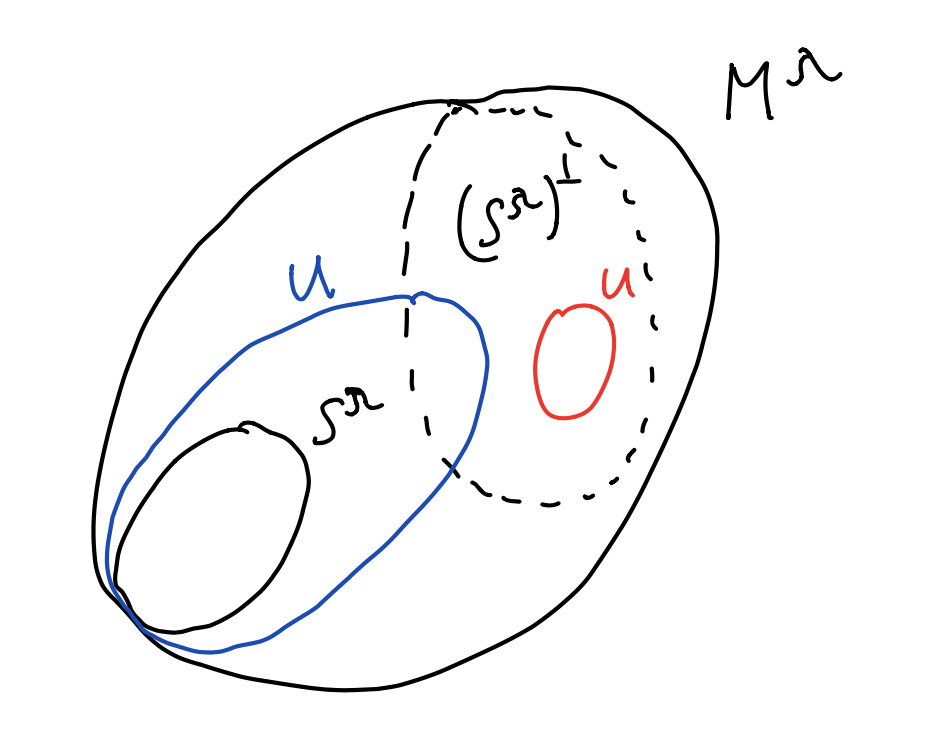
\includegraphics[width=0.5\textwidth]{4.png}
    \caption{Picture for interpreting James' Theorem, courtesy of \cite{Sean}.}
    \label{fig:Figure4}
\end{figure}
\begin{corollary}
    The Specht module $S^{\lambda}$ is irreducible.
\end{corollary}
\begin{proof}[Proof of Corollary]
    Suppose $S^{\lambda}$ has a submodule $0 \neq U \subseteq S^{\lambda}$. Then we can't have $U \subseteq \paren{ S^{\lambda} }^{\perp}$, so we must have $U = S^{\lambda}$, so they are equal. So $S^{\lambda}$ has no proper nontrivial submodules.
\end{proof}
\begin{proof}[Proof of James' Theorem]
    Let's look at all possible $\kappa_t \mathbf{u}$ as $t$ varies over all tableaux of shape $\lambda$ and $\mathbf{u} \in U$. We always have $\kappa_t \mathbf{u} \in U$, since $U$ is a submodule.
    \begin{enumerate}
        \item Case I: Suppose $\kappa_t \mathbf{u} = 0$ for all $t$ and for all $\mathbf{u}$. Then we claim that $S^{\lambda} \perp U$, that is, $\vbrack{ \mathbf{v} , \mathbf{u} } = 0$ for all $\mathbf{v} \in S^{\lambda}$, $\mathbf{u} \in U$. To prove the claim, note that $S^{\lambda}$ is generated by the polytabloids $e_t \coloneqq  \kappa_t \setb{ t }$, so let's look at them. We'll use Signed subgroup invariance:
        \begin{align*}
            \vbrack{ e_t , \mathbf{u} } & = \vbrack{ \kappa_t \setb{ t } , \mathbf{u} } \\
            & = \vbrack{ \setb{ t } , \kappa_t \mathbf{u} } \\
            & = 0.
        \end{align*}
        So $S^{\lambda} \perp U$, and $U \subseteq \paren{ S^{\lambda} }^{\perp}$ as desired.
        \item Case II: Suppose there exists a tableau $t$ (of shape $\lambda$) and a vector $\mathbf{u} \in U$ with $\kappa_t \mathbf{u} \neq 0$. by the Cross-dominance corollary, we have $\kappa_t \mathbf{u} = \alpha e_t$ for some $\alpha \in \cx$. We must have $\alpha \neq 0$, so we can divide and get $e_t \in U$. Since $S^{\lambda}$ is generated by any single polytabloid $e_t$, we get $S^{\lambda} \subseteq U$ as desired.
    \end{enumerate}
\end{proof}

\section{April 27}
\subsection{Blitz}
We have an irreducible representation $S^{\lambda}$ for each $\lambda \vdash n$. Why aren't we done? What's left to prove?
\subsection{Finishing Up Specht Modules}
Let's summarize what we've done so far:
\begin{itemize}
    \item \underline{Cross-dominance lemma}: Let $\lambda , \mu \vdash n$ and let $t^{\lambda}$ and $s^{\mu}$ be tableaux of those respective shapes. Suppose that $\kappa_t \setb{ s } \neq 0$. Then we have the following:
    \begin{enumerate}
        \item $\lambda \trianglerighteq \mu$.
        \item If $\lambda = \mu$, then $\kappa_t \setb{ s } = \pm e_t$.
    \end{enumerate}
    \item \underline{Cross-dominance corollary}: Let $t^{\lambda}$ be a tableau of shape $\lambda$ and let $\mathbf{u} \in M^{\lambda}$. Then $\kappa_t \mathbf{u} = \alpha e_t$ for some $\alpha \in \cx$.
\end{itemize}
\noindent \underline{Summary}: For each partition $\lambda \vdash n$, we have produced the Specht module $S^{\lambda}$ (living inside the mother module $M^{\lambda}$). Let's remind ourselves of our subgoals:
\begin{enumerate}
    \item $S^{\lambda}$ is irreducible. (Thanks, James' Theorem!) Since we know
    \begin{align*}
        \text{number of irreducibles} & = \text{number of conjugacy classes (for all groups)} \\
        & = \text{number of types of cycle decompositions (for $S_n$)} \\
        & = \text{number of partitions of $n$,}
    \end{align*}
    we have the right number of irreducible representations.
    \item The $S^{\lambda}$'s are all distinct. ($S^{\lambda} \neq S^{\mu}$ for $\lambda \neq \mu$.)
\end{enumerate}
First, we determine which Specht modules $S^{\lambda}$ can live in which mother modules $M^{\mu}$.
\begin{theorem}[Homomorphism Dominance]
    Suppose $\theta : S^{\lambda} \to M^{\mu}$ is a nonzero module homomorphism. (Note that $\theta$ is necessarily injective.) Then we have the following:
    \begin{enumerate}
        \item $\lambda \vdash \mu$.
        \item If $\lambda = \mu$, then $\theta$ is multiplication by a scalar $\alpha \in \cx^{\times}$.
    \end{enumerate}
\end{theorem}
\begin{proof}
    \noindent
    \begin{enumerate}
        \item See if you can spot the hole in the following argument:
        $S^{\lambda}$ is generated by the $e_t$, a polytabloid of $\lambda$, where $t$ ranges over tableaux of shape $\lambda$. So there must be a $t$ with $\theta(e_t) \neq 0$ in $M^{\mu}$. But let's invoke $\cx S_n$-linearity:
        \begin{align*}
            \theta(e_t) & = \theta \paren{ \kappa_t \setb{ t } } \\
            & = \kappa_t \theta \paren{ \setb{t} } \\
            & \neq 0.
        \end{align*}
        Now, $\theta \paren{ \setb{ t } } \in M^{\mu}$, which is spanned by the tabloids $\setb{ s_i }$ where the $s_i$ are tableaux of shape $\mu$. Suppose $\theta \paren{ \setb{ t } } = \sum\limits_i \beta_i \setb{ s_i }$, so 
        \begin{align*}
            \theta(e_t) & = \kappa_t \theta \paren{ \setb{ t } } \\
            & = \kappa_t \sum\limits_i \beta_i \setb{ s_i } \\
            & = \sum\limits_i \beta_i \kappa_t \setb{ s_i }.
        \end{align*}
        So we must have some $\kappa_t \setb{ s_i } \neq 0$, so by the Cross-dominance lemma, we get $\lambda \trianglerighteq \mu$. \\\\
        \underline{Problem}: We might not have $\setb{ t } \notin S^{\lambda}$, so it might not make sense to say $\theta \paren{ \setb{ t } }$ (might not be defined). \\\\
        \underline{Patch}: We extend $\theta$ to $M^{\lambda} = S^{\lambda} \oplus \paren{ S^{\lambda} }^{\perp}$ by setting $\theta : \paren{ S^{\lambda} }^{\perp} \to 0$. Now we have a map $\theta : M^{\lambda} \to M^{\mu}$ and its legitimate to say $\theta \paren{ \kappa_t \setb{ t } } = \kappa_t \paren{ \setb{ t } }$.
        \item Suppose $\lambda = \mu$. From above we have
        \begin{align*}
            \theta(e_t) & = \theta \paren{ \kappa_t \setb{ t } } \\
            & = \kappa_t \underbrace{ \theta \paren{ \setb{ t } } }_{ =: \mathbf{u} } \\
            & = \kappa_t \mathbf{u} \in M^{\mu}.
        \end{align*}
        By the Cross-dominance corollary, we get $\theta(e_t) = \kappa_t \mathbf{u} = \alpha e_t$ for some $\alpha \in \cx$. But the single $e_t$ generates $S^{\lambda}$: for any $\mathbf{v} \in S^{\lambda}$, we have $\mathbf{v} = re_t$ for some $r \in \cx S_n$. Then 
        \begin{align*}
            \theta(\mathbf{v}) & = \theta \paren{ r e_t } \\
            & = r \theta \paren{ e_t } \\
            & = r \alpha e_t \\
            & = \alpha r e_t \\
            & = \alpha \mathbf{v}.
        \end{align*}
        So $\theta$ is multiplication by a scalar, as desired.
    \end{enumerate}
\end{proof}
\begin{corollary}
    If $S^{\lambda} \simeq S^{\mu}$, then $\lambda = \mu$.
\end{corollary}
\begin{proof}
    We have nonzero homomorphisms in both directions so by Homomorphism dominance, we get $\lambda \trianglerighteq \mu$, and $\mu \trianglerighteq \lambda$, so $\lambda = \mu$.
\end{proof}
\begin{corollary}
    The Specht modules $S^{\lambda}$ form a complete set of irreducible complex representations of $S_n$.
\end{corollary}
\begin{proof}
    They are all irreducibles, they are all distinct by the corollary above, and we have the right number of them.
\end{proof}
\begin{corollary}
    The mother module decomposes as 
    \begin{equation}
        M^{\mu} \simeq \bigoplus\limits_{\lambda \trianglerighteq \mu} m_{\lambda \mu} S^{\lambda},
    \end{equation}
    for some coefficients $m_{\lambda \mu} \in \z^{\geq 0}$ with $m_{\lambda \lambda} = 1$.
\end{corollary}
\begin{proof}
    Since the $S^{\lambda}$
    s give us a complete set of irreducibles, we know (by Mashcke) that $M^{\mu}$ decomposes into copies of the $S^{\lambda}$. By Homomorphism dominance, the only $S^{\lambda}$'s that could actually appear are those for which $\lambda \trianglerighteq \mu$. And we cannot have more than one copy of $S^{\lambda}$ in $M^{\lambda}$ since otherwise we should have 
    \begin{equation*}
        \dim_{\cx} \left[ \Hom_{\cx S_n} \paren{ S^{\lambda} , M^{\lambda} } \right] > 1,
    \end{equation*}
    contradicting Homomorphism dominance.
\end{proof}
The coefficients $m_{\lambda \mu}$ are called the \textbf{Kostka numbers}, and the theory to find them is described in Sections 2.10 and 2.11 of Sagan \cite{Sagan}, but we won't go into it here.
\begin{example}
    For $S_4$, we have the following decompositions:
    \begin{align*}
        M^{(4)} & = S^{(4)} \\
        M^{(3,1)} & = S^{(3,1)} \oplus ? S^{(4)} \\
        M^{(2,2)} & = S^{(2,2)} \oplus ? S^{(3,1)} \oplus ? S^{(4)} \\
        M^{(2,1,1)} & = S^{(2,1,1)} \oplus ? S^{(2,2)} \oplus ? S^{(3,1)} \oplus ? S^{(4)} \\
        M^{(1,1,1,1)} & = S^{(1,1,1,1)} \oplus ? S^{(2,1,1)} \oplus ? S^{(2,2)} \oplus ? S^{(3,1)} \oplus ? S^{(4)}
    \end{align*}
\end{example}
That's what we get from our new theorems. From previous knowledge of some of these mothers and sons, we can fill in some of the coefficients quickly. For example, we know $M^{(1,1,1,1)}$ is the regular representation, so the coefficients are the dimensions of the irreducibles.

\section{May 4 and May 6}
\subsection{Blitz for May 4}
\begin{enumerate}
    \item Arrange the following partitions of 8 into a Hasse diagram by dominance:
    \begin{equation*}
        (3,2,2,1) , \quad (3,3,2), \quad (4,1,1,1,1), \quad (4,3,1), \quad (5,1,1,1).
    \end{equation*}
    \item The mother module $M^{\lambda}$ is (always, usually, rarely, never) irreducible, and the Specht module $S^{\lambda}$ is (same list) irreducible.
    \item Tell me as much as you can about the decomposition of the mother module $M^{(4,2,1)}$ into Specht modules over $\cx S_n$:
    \begin{equation*}
        M^{(4,2,1)} \simeq ? S^{(?)} \oplus ? S^{(?)} \oplus \underbrace{ \dotsb }_{?} \oplus ? S^{(?)}
    \end{equation*}
\end{enumerate}
\subsection{Blitz for May 6}
\begin{enumerate}
    \item Find $\dim S^{(2,2,2)}$ by listing standard tableaux.
    \item Find  $\dim S^{(3,2,1,1)}$ by Hook formula.
    \item Multiplicity of $S^{(3,1)}$ in each of $M^{(4)}$, $M^{(3,1)}$, and $M^{(1,1,1,1)}$.
\end{enumerate}
\subsection{Standard Tableaux}
There is a really nice way to calculate the dimensions of the Specht module $S^{\lambda}$. You just count the number of \underline{standard} tableaux of shape $\lambda$.
\begin{definition}
    A tableau $t^{\lambda}$ is \textbf{standard} if the entries in each row and each column are increasing.
\end{definition}
\begin{example}
    $\ytableaushort{135,26,4}$ is standard, while $\ytableaushort{156,24,3}$ is not.
\end{example}
\begin{example}
    Let $n \coloneqq  4$ and $\lambda \coloneqq  (2,2)$. We have 2 standard tableaux:
    \begin{equation*}
        \ytableaushort{12,34} , \qquad
        \ytableaushort{13,24}.
    \end{equation*}
\end{example}
\begin{theorem}[Standard Basis Theorem]
    The polytabloids 
    \begin{equation}
        \setb{ e_t \mid \text{$t$ is a \underline{standard} tableau of shape $\lambda$} }
    \end{equation}
    form a basis for the Specht module $\S^{\lambda}$.
\end{theorem}
\begin{corollary}
    To find $\dim_{\cx} S^{\lambda}$, ``just'' count the standard tableaux of shape $\lambda$.
\end{corollary}
\begin{example}
    The Specht module $S^{(2,2)}$ of $S_4$ has dimension 4 as we calculated in Homework.
\end{example}
The proof of the Standard basis theorem is nontrivial: you have to extend the notion of partitions to compositions, extend dominance to tabloids, introduce column tabloids and something called a Garnir element, and then give separate proof for linear independence and spanning. Refer to Section 2.5 in Sagan \cite{Sagan}.
\subsection{The Hook Formula}
As beautiful as the Standard basis theorem is, it's not very easy in general to count standard tableaux and determine the dimension of $S^{\lambda}$.
\begin{example}
    Find $\dim_{\cx} S^{(3,3,1)}$.
    \begin{proof}[Solution]
        Since both the columns and the rows must be increasing, we have no choice but to put 1 in the upper left corner. 
        \begin{equation*}
            \begin{ytableau}
                1 & ?  & ?  \\
                ?  & ?  & ?  \\
                ?
            \end{ytableau}
        \end{equation*}
        From here we have two cases:
        \begin{itemize}
            \item Case I: We can put 7 on the single box in the third row. This forces 6 to be in the $(2,3)$ spot (read like matrix entries):
            \begin{equation*}
                \begin{ytableau}
                    1 & ?  & ?  \\
                    ?  & ?  & 6  \\
                    7
                \end{ytableau}.
            \end{equation*}
            This leaves us with four spots to put 2, 3, 4, and 5 in. To narrow this down, let's fix 3,4, and 5 in the $(1,3)$ spot:
            \begin{itemize}
                \item If we fix 3, then we have only 1 remaining choice for the rest of the numbers.
                \item If we fix 4, then we have 2 choices to place the remaining numbers.
                \item Similarly, fixing 5 gives us 2 choices.
            \end{itemize}
            This gives us $1 + 2 + 2 = 5$ choices for Case I.
            \item We can put 7 in the $(2,3)$ spot:
            \begin{equation*}
                \begin{ytableau}
                    1 & ?  & ?  \\
                    ? & ?  & 7  \\
                    ?
                \end{ytableau}.
            \end{equation*}
            Note that we can place 2 and 3 in the green region, and 4, 5, and 6 in the orange region:
            \begin{equation*}
                \begin{ytableau}
                    1 & *(green) ? & *(orange) ?  \\
                    *(green) ? & *(orange) ? & 7  \\
                    *(orange) ?
                \end{ytableau}.
            \end{equation*}
            This gives us $2! \times 3! = 12$ choices, but that's not all! Let's place 2 in the $(1,2)$ spot. Then we can actually place 3 to the right of 2. This forces 4 right below 1, and so we have two spots to put 5 and 6 in:
            \begin{equation*}
                \begin{ytableau}
                    1 & 2 & 3  \\
                    4 & *(orange) ? & 7  \\
                    *(orange) ?
                \end{ytableau}.
            \end{equation*}
            This gives us an additional 2 choices. Lastly, we can stack 1, 2, and 3 in the first column, which forces 4 to the right of 1:
            \begin{equation*}
                \begin{ytableau}
                    1 & 4 & *(green) ?  \\
                    2 & *(green) ? & 7  \\
                    3
                \end{ytableau}.
            \end{equation*}
            Again, this gives us 2 more choices.
        \end{itemize}
        Putting this all together, we have $5 + 12 + 2 + 2 = \boxed{21}$ standard tableaux, so $\dim_{\cx} S^{(3,3,1)} = 21$. 
    \end{proof}
    Obviously, this process is prohibitively difficult for larger partitions. However, there is another, easier way to determine the dimension.
\end{example}
\begin{definition}
    Let $\lambda \vdash n$ and let $Y$ be a Young diagram of shape $\lambda$. For each box $b \in Y$, define the \textbf{hook length} $h(b)$ to be the total number of boxes in the ``hook'' extending down and to the right of $b$, including $b$ itself.
\end{definition}
\begin{example}
    \noindent
    \begin{itemize}
        \item For the box below, $h(b) = 6$.
        \begin{equation*}
            \begin{ytableau}
                \, & \, & \, \\
                \circ & \ast & \ast \\
                \ast & \, \\
                \ast & \, \\
                \ast
            \end{ytableau}
        \end{equation*}
        \item Each box below is labeled with its hook length.
        \begin{equation*}
            \ytableaushort{532,421,1}
        \end{equation*}
    \end{itemize}
\end{example}
\begin{theorem}[Hook Formula]
    Let $Y$ be a Young diagram of shape $\lambda \vdash n$. Then $\dim_{\cx} S^{\lambda}$ (which is the number of standard tableaux) is given as follows:
    \begin{equation}
        \dim_{\cx} S^{\lambda} = \frac{n!}{\prod\limits_{b \in Y} h(b) }.
    \end{equation}
\end{theorem}
\begin{example}
    \noindent
    \begin{itemize}
        \item Let $\lambda \coloneqq  (3,3,1) \vdash n\coloneqq  7$. From the diagram above, we have 
        \begin{equation*}
            \frac{ 7 \times 6 \times \cancelto{1}{5} \times \cancelto{1}{4} \times \cancelto{1}{3} \times \cancelto{1}{2} \times 1 }{ \cancelto{1}{5} \times \cancelto{1}{3} \times \cancelto{1}{2} \times \cancelto{1}{4} \times 2 \times 1 \times 1} = \frac{7 \times 6}{2} = \boxed{21.}
        \end{equation*}
        This confirmed our work above, but it's much easier.
        \item Let $\lambda \coloneqq  (n) \vdash n$ or $\lambda \coloneqq  \paren{ 1 , 1 , \dotsc , 1 } \vdash n$. Either way, we get
        \begin{equation*}
            \ytableausetup{boxsize = 3em}
            \begin{ytableau}
                n & n-1 & \cdots & 1
            \end{ytableau},
            \qquad
            \begin{ytableau}
                n \\
                n-1 \\
                \vdots \\
                1
            \end{ytableau},
        \end{equation*}
        and so $\dim_{\cx} S^{\lambda} = 1$, as we knew because $S^{\lambda}$ is the trivial representation or the sign representation, respectively.
        \item Let $\lambda \coloneqq  (n-1,1) \vdash n$, and let $Y$ be the Young diagram associated to $\lambda$. Filling $Y$ with its hook numbers gives us
        \begin{equation*}
            \begin{ytableau}
                n & n-2 & \cdots & 1 \\
                1
            \end{ytableau},
        \end{equation*}
        and so the hook formula gives us
        \begin{align*}
            \dim_{\cx} S^{\lambda} & = \frac{n!}{ \prod\limits_{b \in Y} h(b) } \\
            & = n! \times \inv{ \paren{ n \times (n-2)\times (n-3) \times \dotsm \times 1 \times 1 } } \\
            & = n! \times \frac{n-1}{n!} \\
            & = n-1,
        \end{align*}
        as we knew because $S^{\lambda}$ is the standard representation (perm $-$ triv). We get the same result for $(2,1,\dotsc,1)$.
    \end{itemize}
\end{example}
\begin{remark}
    David \cite{David} made a very astute observation at this point about the dimensions of the Specht modules. In the Homework, we have been computing the characters of the Specht modules and arranging the characters in order of dominance. Then we proved that the Hasse diagram for any partition looks the same flipped as it does right side up (even when the diagram isn't totally ordered). The gist of the idea is that when $\lambda \trianglerighteq \mu$, taking the ``transpose'' of the partitions reverses the dominance. By ``transpose'' we mean the partition pertaining to the Young diagram transposed, and this new partition is called the \textbf{conjugate partition}. David's remark was this: dimensions of the Specht modules come in pairs, since you can always tensor one of them up with the sign representation to get another non-isomorphic Specht module. However, if the Young diagram is \underline{symmetric}, then tensoring up with the sign representation gives you back the same Specht module, so you don't get an extra one. Whether this observation is true or not will have to be dealt with outside of the class, but it seems like a really neat idea.
\end{remark}
\begin{proof}[Proof of the Hook Formula]
    Let's take a random tableau of shape $\lambda$ and test whether it is standard. \\\\
    \underline{Key observation}: Let's look at any single hook, like this one:
    \begin{equation*}
        \ytableausetup{boxsize = 1.5em}
        \begin{ytableau}
            \, & \, & \, \\
            \circ & \ast & \ast \\
            \ast & \, \\
            \ast & \, \\
            \ast
        \end{ytableau}
    \end{equation*}
    If the tableau is standard, then the circle should be smallest number in the whole hook. We'll say that this hook is \underline{standard}. Since we arranged the numbers randomly, the chance that the example hook above is standard is $\frac{1}{6}$, and in general, $\frac{1}{h(b)}$.
    
    Now, the whole tableau is standard if and only if every individual hook is standard. So we can find the \underline{probability} that the tableau is standard by multiplying the probabilities of each hook being standard. That gives a probability of 
    \begin{equation*}
        \frac{1}{\prod\limits_{b \in Y} h(b) }.
    \end{equation*}
    Since there are $n!$ tableaux in all, we then know that 
    \begin{equation*}
        \frac{n!}{\prod\limits_{b \in Y} h(b) }
    \end{equation*}
    of them are standard.
\end{proof}
\begin{remark}
    Pros:
    \begin{enumerate}
        \item This proof is cool.
        \item This proof is illuminating.
        \item This proof is short.
        \item This proof has an illustrious pedigree. Thanks, Don Knuth, who is certainly $A$-list celebrity and also bequeathed us TAOCP, for which he created TeX, from which \LaTeX emerged from.
    \end{enumerate}
    Con: This proof is \underline{wrong}! Why, because the events aren't independent! Let's work it through.
\end{remark}
\begin{example}
    Let $\lambda \coloneqq  (2,2) \vdash n\coloneqq  4$. Let's look at the hook lengths:
    \begin{equation*}
        \ytableaushort{32,21}.
    \end{equation*}
    By our theory, $\frac{1}{3}$ of the 24 tableaux should have a standard first hook. Let's list them:
    \begin{align*}
        \ytableaushort{12,34} & \quad \ytableaushort{13,24} \quad \ytableaushort{12,43} \quad \ytableaushort{13,24} \\[0.5em]
        \ytableaushort{14,23} & \quad \ytableaushort{14,32} \quad \ytableaushort{23,41} \quad \ytableaushort{24,31}
    \end{align*}
    Again by our theory, $\frac{1}{2}$ of those should have a standard second hook (the vertical one starting in position $(1,2)$). Let's list those:
    \begin{equation*}
        \ytableaushort{12,34}, \quad \ytableaushort{13,24}, \quad \ytableaushort{12,43}.
    \end{equation*}
    This shows that the events
    \begin{align*}
        A & \coloneqq  \text{``first hook standard''} \\
        B & \coloneqq  \text{``second hook standard''}
    \end{align*}
    are \ita{not} independent:
    \begin{align*}
        P(A \cap B) & = \frac{3}{24} = \frac{1}{8}, \\
        P(A) \times P(B) & = \frac{1}{3} \times \frac{1}{2} = \frac{1}{6}, \\
        \frac{1}{8} & \neq \frac{1}{6}.
    \end{align*}
\end{example}
To resolve this, turn to (where else?) Sagan \cite{Sagan}, Section 3.10. It took 40 years to produce a good bijection that Sagan concedes is ``still somewhat involved.'' In fact, if you do happen to find an easy-to-understand proof, the greater mathematical community would be quite interested to hear it!
\newpage
\section{Appendix}
\subsection{Frobenius' Biography [from Handout]}
Ferdinand Georg Frobenius (October 26, 1849 - 1917) was born near Berlin. He started university at G\"ottingen but returned to Berlin, where he studied under Kronecker, Kummer, and Karl Weierstrass. His doctoral thesis, supervised by Weierstrass, was on differential equations. He worked in Z\"urich for 17 years until Kronecker died and Weierstrass brought Frobenius back to lead Berlin.

He proved the Sylow theorems for abstract groups (Sylow only did it for permutation groups), and his proof is one of those frequently used today. He also made fundamental contributions to number theory, extending Dirichlet's results.

Character theory predates representation theory: Frobenius developed character theory in letters to Dedekind starting in 1896. Representations were born in 1897, and in 1897 - 1899 Frobenius introduced induced representations, tensor products, and Reciprocity.

In a letter to Dedekind on his semi-birthday, April 26, 1896 Frobenius gave the irreducible characters for $A_4$, $A_5$, $S_4$, $S_5$, and $PSL(2,7)$ of order 168. By 1900 he did all of $S_n$ and by 1901, all of $A_n$.

However, Frobenius was ``choleric, quarrelsome, and given to invectives.'' His standards were so austere that Berlin, the old home of pure math, gradually lost ground to the new ideas G\"ottingen, led by Klein.

\newpage
\phantomsection
\addcontentsline{toc}{section}{References}
\begin{thebibliography}{99}
    \bibitem{Dummit} Dummit, David S. and Richard M. Foote. \ita{Abstract Algebra, $3^{rd}$ Ed.} Wiley, 2004.
    \bibitem{Leon} Kim, Leon. For making the special quotient macro.
    \bibitem{Desmos} Desmos Online Graphing Calculator.
    \bibitem{Rami} Allaf, Rami.
    \bibitem{Sean} Zhou, Sean. For sharing his completed notes with me.
    \bibitem{David} Haber, David. For showing me the \textsf{ytableau} package.
    \bibitem{Sagan} Sagan, Bruce E. \ita{The Symmetric Group: Representations, Combinatorial Algorithms, and Symmetric Functions, $2^{nd}$ Ed.} Springer, 2001.
\end{thebibliography}

\end{document}